\documentclass[10pt, b5paper]{report}
\usepackage[utf8]{inputenc}
\usepackage{lscape}   % Make a page in landscape format \begin{landscape}
\usepackage{colortbl} % To color table cells
\usepackage{color} % Able to change textcolor
\usepackage[table]{xcolor}
\usepackage{longtable}
\usepackage{graphicx} % Able to add pictures
\usepackage{parskip}  % Separate paragraphs with a blank line
                      % rather than using indentation
\usepackage{hyperref} % Support for hyperlinks
\usepackage[protrusion=true,expansion=true]{microtype} % Improve justification
\usepackage{subfigure}
\usepackage{caption}
\usepackage{float}
\usepackage{afterpage}
\usepackage{lipsum}
\usepackage{wrapfig}
\usepackage{enumerate}
\usepackage{natbib}
\usepackage[colorinlistoftodos]{todonotes}
\usepackage{mdwlist}
\usepackage{array}
\usepackage{listings}
\usepackage[english]{babel}
\usepackage{fancyhdr}
\usepackage{multirow}
\usepackage[margin=0.9in]{geometry}
\usepackage{listings}
\usepackage[toc,page]{appendix}
\usepackage{enumitem}
\usepackage{tocbibind}
\usepackage{booktabs}
\usepackage{stackengine}




%-------- Chapter Styling -----------
\usepackage[T1]{fontenc}
\usepackage{titlesec}
\definecolor{gray75}{gray}{0.75}
\newcommand{\hsp}{\hspace{20pt}}
\titleformat{\chapter}[hang]{\Huge\bfseries}{\thechapter\hsp\textcolor{gray75}{|}\hsp}{0pt}{\Huge\bfseries}

%------ DIV -------------------------
\renewcommand*\contentsname{Table of Contents}
\hypersetup{%
	pdfborder = {0 0 0}
}

\begin{document}
	\pagenumbering{gobble}
	\thispagestyle{empty}
	\begin{titlepage}
\begin{center}
	
	\vspace{2cm}

	{\Huge "Tell Me Who You Are and I Will}\\[0.4cm]
	{\Huge Tell You Your Lock Pattern"} \\[5cm]

	%Can you keep a secret?
	%Tell me who you are, and I will know your password.

	{\Large Master Thesis by Marte Dybevik Løge} \\[0.4cm]
	{\Large Norwegian University of Science and Technology}\\

	\vspace{9.0cm}

			%\includegraphics{pics/ntnu-logo2.png}

	%\vspace{3.0cm}

	{\Large Supervisor: Lillian Røstad} \\ [0.2cm]
	{\Large Co-supervisor: Per Thorsheim} \\ [0.2cm]
	
\end{center}
\end{titlepage} \thispagestyle{empty}
	% !TEX root = main.tex

{\centering 

	{\Huge Abstract}

	\vspace{1cm}

	This is the abstract....T his is the abstract.... This is the abstract.... This is the abstract....This is the abstract.... This is the abstract.... This is the abstract....This is the abstract.... This is the abstract.... This is the abstract.... This is the abstract....

}

\clearpage


{\centering 

	{\Huge Sammendrag}

	\vspace{1cm}

	Her kommer det er sammendrag på norskHer kommer det er sammendrag på norskHer kommer det er sammendrag på norskHer kommer det er sammendrag på norskHer kommer det er sammendrag på norskHer kommer det er sammendrag på norskHer kommer det er sammendrag på norskHer kommer det er sammendrag på norskHer kommer det er sammendrag på norskHer kommer det er sammendrag på norskHer kommer det er sammendrag på norskHer kommer det er sammendrag på norskHer kommer det er sammendrag på norsk
	
}

	
 \thispagestyle{empty}
	\tableofcontents \thispagestyle{empty}
	\listoffigures \thispagestyle{empty}
	
	\cleardoublepage
	\begingroup
	\makeatletter
	\let\ps@plain\ps@empty
	\makeatother

	\pagestyle{empty}
	\listoftables
	\cleardoublepage
	\endgroup

	\listoftodos
	% !TEX root = main.tex

\section*{General TODOs}
	
	%\todo[inline, color=red!70] -- Major Error, Fix right away. Type of error not specified. 
	%\todo[inline, color=yellow!80] -- Skrivefeil eller forbedre skriving.
	%\todo[inline, color=green!60] -- Note to self
	%\todo[inline, color=blue!60] -- Det er noe som mangler.
	%\todo[inline, color=orange!80] -- Something, not specified.
	
	Dette er en liste med generelle todos som gjelder hele reapporten eller ikke tilhører et spesifikt kapittel. 

	\todo[inline, color=yellow!80]{Skal jeg skrive "Android Pattern Lock" med uppercase, eller skal jeg skrive "Android pattern lock"?}

	\section*{Abbrevations}

	IT = Information Technology

	ALP = Android Lock Pattern

	


	\pagenumbering{arabic}		

	% !TEX root = ../main.tex
\chapter{Introduction}\label{chap:introduction}
	
	\clearpage
	\section{Background and Motivation} \label{sec:backgroundandmotivation}

		As mobile devices play a significant role in our everyday life, it makes it an interesting target device because it contains a lot of sensitive information. The use of mobile phones has changed in terms of capability, interaction and context of use and, therefore, the increased need for higher security. Mobile phones are not just capable as a tool for simple communication, but also a tool to perform our daily tasks like paying bills and keeping up with our social life. The smartphone are becoming an integrated part of our daily life and is becoming a device keeping a lot of sensitive information about your professional and private life.

		Screen locks are used as a protection mechanism to prevent leakage of sensitive data from mobile devices. The history of locking mechanisms was often a solution solely to prevent accidental use while current mobile phones require protection to secure the potentially vast amount of private data that we keep on our mobile devices. The most common mechanisms for protection today is the use of locking mechanisms like PIN codes, fingerprints, and pattern locks. The screen lock mechanism is also a form of a password, e.g. a secret only you know to get access to a resource. The problem with passwords on mobile devices has three different aspects. First, people find it hard to remember long and secure password. Second, the way we interact with touch screens makes it hard to type long text-based passwords on a small mobile keyboard. Third, we interact with the phone many times a day, making the overhead in time used to unlock the smartphone very high when using a long and complex password.

		Looking at passwords in general, passwords are often a user-selected secret that are connected to you as a person. When creating a password, people tend to create a password that is an association to something they know or recognize; passwords are more than just words and numbers. The way people choose their password cause the passwords we make to be predictable and therefore being insecure. People tend to select PIN codes forming a date, or an alphanumeric password consisting of your name or perhaps your favorite sports team. This predictability is a cause of how people cope with the problem of remembering passwords, e.g. the shortcomings with alphanumeric passwords. 

		Because of the shortcomings with alphanumeric passwords \cite{UnixPasswords}, there is an increased interest in graphical passwords. Graphical passwords were fist a suggestion for motivating users to create long and memorable passwords and, therefore, more secure started by the assumption that pictures are easier to remember and more secure than words and numbers \cite{DeAngeli}. Graphical passwords look like a promising alternative to text-based passwords, as it supports users to remember and make more complex passwords, offering better usability and higher security. The way of interacting with the smartphone also seem as a well-suited platform for a graphical password because graphical passwords often use direct manipulation of graphical elements instead of typing small letters and numbers. One of the graphical passwords in rapid use is the Android Pattern Lock released on the Android platform by Google in 2008. The Android Pattern Lock is a graphical password that enables the users to connect dots from a 3$\times$3 grid forming a password. Since its release, there has been much discussion of its security, but few researchers have conducted scientific research on the Android Unlock Pattern. Compared to PIN code that are often used as a screen lock on mobile devices, PIN codes have a total of 10.000 possible combinations while the Android pattern lock have a total of 389.112 possible combinations. By the first sight, pattern lock looks like a promising mechanism for mobile devices. The problem is not just the theoretical password space, but rather the password space in practice. In 2013, a research group conducted the first large-scale user study on the Android Unlock Patterns \cite{Uellenbeck}. The outcome of the research was an analysis of 2900 user-selected patterns. They found bias in the pattern making process claiming that the scheme are less secure than its stated theoretical password space.

		Taking a closer look at the Android pattern lock; it is only dots and arrows forming a password. How can this be connected to you as a person like PIN codes and alphanumeric passwords? Researchers have found bias and predictable behavior in creation of password cross different password scheme, but there are few researchers that have studied the human factors in the password creation process. Is predictable behavior a general observation, or is the predictable behavior conditioned by who we are? In this study it will be collected a set of user-selected patterns with a corresponding set of human properties to be able to observe if who we are influences our choice in graphical passwords. 

	\clearpage
	\section{Methodical Approach} \label{sec:researchmethods}

		This section will give a brief introduction to the methodical approach. The methods is divided into four steps starting with reviewing the literature based on the background and motivation. The next step is to define a hypothesis that reflects the theory that I want to answer. To be able to answer the hypothesis, it is performed a large scale of quantitative data that finally can be analyzed to be able to accept or reject the proposed hypothesis. 

		\subsection{Reviewing the Literature}\label{sec:methodliteraturereview}

	    A literature review is often used for two main purposes. {\it First}, it is useful to look for a suitable research idea and discover relevant material about any possible research topics. {\it Second}, the second part often begin once a research topic is chosen, where the aim is to gather and present evidence to support that the research can produce new knowledge.

	    There is a broad range of sources to be used in the literature review, for example, books, journal articles, and conference papers. Books are often based on well know facts with a broad scope. Journal articles and conference papers are more exploratory and are useful for finding information on the current thinking and research in the area. All published journals and conference proceedings needs to be reviewed carefully. It is important to use the sources that is considered to publish quality research and that they provide sufficient quality control on the published research. Some highly rated journals in information systems and computing is: ACM \cite{ACM}, IEEE \cite{IEEE}, and Springer \cite{Springer}. When using conference papers, it can often be useful to read something about their review procedures and their quality requirements. Besides the publication source, it can be helpful to look at the number of citations used. If a research paper has many citations, it may be an indication of it quality.

	    When reviewing the literature, it would be too time consuming to read all the papers from the start to the end. To be able to select relevant research, it is preferable to look at the abstract first that should include information about the research motivation, the methods used, as well as the results. If the abstract were promising, the review continues by reading the results and methods chapters. If the research is very interesting, it might be valuable to read the whole publication from start to end.

	    Before searching for relevant literature, it is important to define keywords that can narrow the search down to obtain information that is relevant according to the research that is being conducted. The keywords can be combined when searching in different digital libraries. When relevant literature is found, it is important to set a list of quality criteria that until now have been discussed.
	    The selected quality criteria that are chosen is listed in Table~\ref{tab:QualityCriteria}.

	      \begin{table}[H]
	        \centering
	        \begin{tabular}{| l | p{10cm} |}
	          \hline
	          {\bf \#} & {\bf Quality Criteria} \\ \hline
	          QC 1 & The research is published in a known digital library, journal or conference\\ \hline
	          QC 2 & There is a clear statement of the aim of the research\\ \hline
	          QC 3 & The study is cited by other researchers\\ \hline
	          QC 4 & There is a clear description of the method used in the study\\ \hline
	          QC 5 & If the research includes an experiment, user study, or other research strategies, there should be a reasonable sample size used. \\ \hline
	        \end{tabular}
	        \caption{Quality criteria for literature review}
	        \label{tab:QualityCriteria}
	      \end{table}

	    Sometimes, there will be resources needed that is not published in a well known journal. Example is important content only found on web pages and blog posts. The use of content from web pages should be avoided if it is possible to find published research instead. It a web page is used as a refernce it is clearly stated in the bibliography when the site was last accessed. 


		\subsection{Collecting Quantitative Data}
			%Hvorfor kvantitativ og ikke kvalitativ??

			The data collected in the this research needs to collect large amounts of data, and the same time keep the answers anomyous. An online survey does support the ability to collect large amounts of data without the need for too much manual work. Using and online survey also makes it possible to reach people living at different geographical locations.

			When collecting patterns and other information about the respondents it is important to not be able to track an respons back to the respondent. The answer should be anonymous due to ethical concerns. An online survey will support the possibility to keep answers anonymous because I do not have to directly interact with the respondents, nor do I know who actually responds. This sampling techniqe is a self-selection sampling techniqe \cite{empiriske}, meaning that anyone that wants to participate can answer. This techniqe are selected to support the requirements of anonymity where no knowledge of who the particpants are beside the provided information from the survey. 

			Chapter \ref{chap:experiment} will give a detailed description of the survey design; the questions asked and the layout and structure of the survey.


		\subsection{Analyzing Quantitative Data}

	\clearpage
	\section{Hypothesis}\label{sec:hypothesis}

		This section will be an elaboration of the hypothesis to be tested by performing an experiment.

		{\renewcommand\labelitemi{}
			\begin{itemize}
	  		\item \texttt{$H_{0}$: Human properties have no influence on users choice of \\graphical passwords}
	  		\item \texttt{$H_{1}$: Users choice of graphical passwords are influenced by \\the human properties of the user}
	  	\end{itemize}
	  }

	  The hypothesis to be tested is referred to as the null hypothesis (abbreviated $H_{0}$). We start with the assumption that the null hypothesis is true; human properties have no influence on users choice of graphical passwords. Along with $H_{0}$ it is stated an alternative hypothesis (abbreviated $H_{1}$). The alternative hypothesis states that users choice in graphical passwords is influenced by the human properties of the user. If the null hypothesis is rejected, we accept the alternative hypothesis. The hypothesis will be tested by performing an experiment by collecting Android lock patterns and a set of human properties to the creators of the patterns. The experiment will be observing if a set of human properties will cause an effect in the patterns created.

	  If the hypotehesis is accepted, it would mean that it is very likeley that there is no correlation between human properties and the choice of graphical passwords. In other words, predictable behaviour when studying password is an general observation not caused by human properties.

		The aim of the research is to answer the overall hypothesis, but there is also some further supplementary questions that is interesting to include in this research. They will require a discussion besed on the results found when answering the hypothesis combined with the results from the literature study.

	  {\renewcommand\labelitemi{}
			\begin{itemize}
	  		\item \texttt{$Q1$: How does the result impact the security of the Android \\Lock Pattern?}
	  		\item \texttt{$Q2$: How is observed behaviour of the Android Pattern lock scheme \\compared to other screen locks used on mobile devices?}
	  	\end{itemize}
	  }

	  {\bf Q1:} The hyphotesis are closely related to a security evaluation. Any predictable behaviour when looking at passswords is a violation of the security. If th hypothesis is either accepted or rejected, it is intersting to see if it impacts how we evaluate the security of the scheme. 

	  {\bf Q2:} As described in the background and motivation, predictable behaviour is found in a varity of password schemes. The interesting question is if the human behaviour related to Android Lock Patterns is compareable to what is observed in other password mechanims used on mobile devices. 


	\section{Limitations}
		When conduction research there is often a scope and corresponding limitations. This section will give an overview of the limitations that need to be red before reading this document. This first part will give a brief overview of the limitations when looking at the overall research objective; the hypothesis. The second part looks at limitations of the selected methodical approach. 

		\subsection{Hypothesis}
	  	The proposed hypothesis will have some limitations. {\it First}, the hypothesis do not include all potential human properties. If the results of the statistical test are accepting the alternative hypothesis, the results are not valid for proving a correlation between users choice in graphical passwords and human properties that are not selected in this research. {\it Second}, the hypothesis does neither prove that human choices based on the human properties is valid for all graphical password schemes. The selected graphical password scheme is the Android Unlock Pattern. Chapter \ref{chap:results} will include a detailed description of the human properties included in the experiment.

	  \subsection{Methodical Approach}
	  	When conducting the experiment, it is not possible to have control of the participants due to ethical concerns. In an experiment is is often desired to have a control group to validate the collected data. To be able to use a control group I would have to ask people about their real patterns, that is not desired for security reasons. This experiment will only be able to see the cause and effect on the patterns collected in this research.

	  	The collected data is also collected over the Internet, meaning that I as a researcher have no control on who people are and if answers provided by participants are committed honestly. As mentioned in the elaboration of the methodical approach, I should not be able to track whom participating in the study due to ethical concerns. It is neither desirable to take an pen-and-paper approach due to both ethical concerns and the time available for collecting an reasonable amount of data. The data is collected to be as representative as possible to the real world without violating any privacy concerns. 
	
	\section{Contributions} \label{sec:contributions}
		% ---> Hva bidrar jeg med?
		% The results from this study can further be used to evaluate the security of the Android Unlock Pattern. If there is a correlation between users choice in Android Unlock Patterns and the users human properties, it can be used to make dictionary attacks by predicting user's pattern locks. An ability to predict user's choice in locking patterns is a reduction in the scheme's security. 

		When conducting research you want to contribute with knowledge and answer questions that no other person have been answered before. This research want to test a new theory formed as a hypothesis to add to the body of knowledge as the main contribution.

		In the process of formulating the hypothesis, published literature concerning graphical passwords have been reviewed. The reviewed literature is up to date and gives an summary of the latest published work on graphical passwords, in particular research concerning the Android Pattern Lock. 

		To be able to collected the data, there is developed a survey for collecting data on mobile devices. The science and work behind the survey can support other researchers to see how data collection can be performed over the Internet, in particularly how to collect user-selected passwords. It is not a straight forward process to collect passwords due to ethical concerns. 

		The data collected in the survey is by far one of the first large-scale collections of graphical passwords with the detailed information about the users.

	\section{Thesis structure} \label{sec:structure}

		{\bf Chapter 2: Related Work on Graphical Passwords}
		An introduction to the related work that have been published on graphical passwords. 

    {\bf Chapter 3: Experiment}

    {\bf Chapter 4: Results}

    {\bf Chapter 5: Discussion}

    {\bf Chapter 6: Conclusion and Future Work}



	% !TEX root = ../main.tex
\chapter{Background Theory and Related Work}\label{chap:relatedwork}
  
  This chapter looks into the background theory needed for futher reading this thesis, as well as providing an insigh to related work.  
  The chapter starts with Section \ref{sec:shortcomings}, providing an overview of the shortcomings with text-based passwords; the origin of graphical passwords. Section \ref{sec:historygraphicalpasswords} looks at graphical passwords from a historical point of view. When did it all start, and where are we now? The section describes and visualises graphical passwords schemes proposed over the past years until today. Section \ref{sec:evaluation} are looking at research evaluating different graphical password schemes from usability and security point of view. Section \ref{sec:humanfactors} looks at graphical passwords focusing on the human aspects of security, as well as introducing some material from psychology. As mobile devices is a crucial part of our daily lives, Section \ref{sec:pwmobiledevices} are looking into graphical passwords and mobile devices. At last, Section \ref{sec:alp} looks particularly into one of the most commonly used graphical passwords schemes on mobile devices; the Android Pattern Lock.
	% !TEX root = ../main.tex
\section{Shortcomings of Text-Based Authentication} \label{sec:shortcomings}

  User authentication is a central part of security systems. Despite the extensive number of options for authentication, text-based passwords remain the most common authentication scheme. Text-based authentication is the authentication scheme widely adopted because it is easy and inexpensive to implement, and users are familiar with the scheme. Text-based authentication also avoids the privacy issues raised by the use of biometric authentication, as well as preventing the need for a physical security device used in token-based authentication schemes. However, text-based authentication suffers from both security and usability disadvantages. As users need to remember an increasing number of passwords, users adopt bad password habits. The term {\it habit} is often a bad thing when talking about security. A habit is often hard to change and is often predictable because it tends to occur in similar situations repeatedly.

  Password reuse is one of the known password habits among users, caused by human limitations for being able to remember text-based passwords.Another habit introduced as a cause of dealing with the problem of remembering passwords is to create short and meaningful passwords that are easier to remember. However, a consequence of creating short passwords is a vulnerability for brute-force attacks, introducing a security risk. Furthermore, having an expanding number of accounts requires users to manage a set of different passwords across multiple devices. The problem is not just to remember all the required passwords, but also to remember which passwords belong to which account or device. The increased number of accounts and devices is an another cause for users to reuse passwords across multiple accounts and devices.

  One of the first large-scale studies on web password habits was conducted in 2007 by Microsoft Research \cite{habits1}. They analyzed text-based passwords used by 544.960 Internet users over a period of 3 months. In order to collect the passwords, Microsoft used a Windows Live Toolbar observing activities like login frequency. They were also able to observe how many unique passwords each user had and how the passwords were used across separate URLs. Microsoft observed that a typical user has an average of 7 distinct passwords. Out of the seven unique passwords, five of them were re-used on different web pages. An estimate of the average number of accounts per user was estimated to 25 accounts per user.

  Password schemes have what is called a {\it theoretical password space} that is the number of possible combinations of passwords that a user can make. Research has reported that when creating passwords, users to not utilize the entire password space, but uses only a subset of the conceivable password combinations. The password space in use can be seen as the {\it practical password space}, making the practical password space less than the theoretical password space (Figure \ref{fig:memorable}). The selected passwords show that the security of a password scheme relates to its practical password space rather than its theoretical password space.

    \begin{figure}[H]
      \centering
      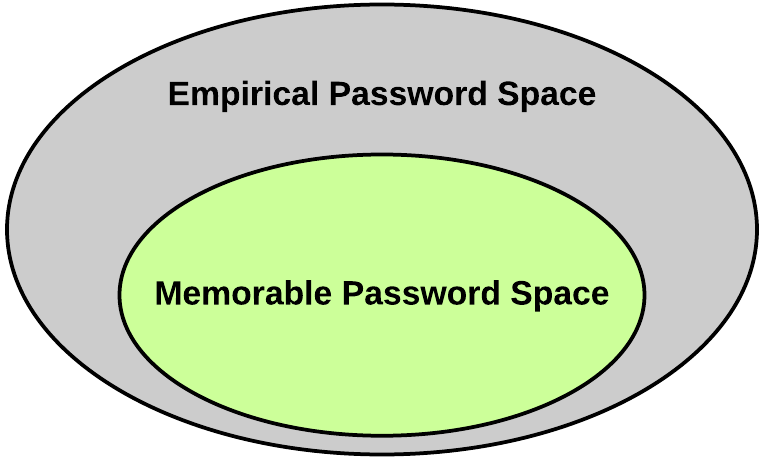
\includegraphics[scale=0.55]{pics/review/EmpiricalVsPractical.png}
      \caption{Theoretical password space vs. Password space in practice}
      \label{fig:memorable}
    \end{figure}

  In a case study of 14.000 Unix passwords, a research group found that 25\% of the passwords were a group of words forming a dictionary of $3\times10^{6}$ words \cite{UnixPasswords}. This dictionary shows that an attacker can have a relatively high success rate for an attack, despite the fact that there are roughly $2\times10^{14}$ 8-character passwords consisting of digits, and upper and lower case letters. As a result of people choosing weak passwords that are easier to remember, a significant number of user-chosen passwords falls into a small dictionary, e.g. the password space in practice \cite{Tao}. A well-designed dictionary is considered to be a tiny subset of the full password space, e.g. the theoretical password space, which further may be prioritized according to the likelihood for a password to be chosen. It is, therefore, commonly stated that the security of a password scheme is related to the size of its password space in practice, rather than its theoretical password space. The high success rate of dictionary attacks against text-based passwords is considered to be a significant cause of the recall capabilities of humans and how they choose their passwords.

  As a result of the shortcomings of text-based authentication, graphical authentication is getting increased attention as an alternative to text-based authentication. Graphical passwords are attempting to help the users to be able to create secure passwords that are also easy to remember. Instead of consisting of text and numbers, graphical passwords make use of images and visual objects in the authentication process. When comparing the use of text against the use of visual objects, the human brain is more capable of remembering images than text \cite{DeAngeli}. As a consequence of humans being more capable of recognizing images, users will be more capable of creating more complicated passwords that are harder to guess.

  The next section will look further into the history of graphical passwords; when did it all start and what does the situation look like today?
  
	% !TEX root = ../main.tex
\section{The History of Graphical Passwords} \label{sec:historygraphicalpasswords}
	 
  This section will review related work on graphical passwords from a historical point of view. The graphical password schemes reviewed will provide an elaboration of how the scheme works as well as a graphical illustration of its design. Like text-based passwords schemes, graphical password schemes are also a knowledge-based authentication scheme, e.g. ``something you know''. Since it all started around 1996, there have been many suggestions for graphical password schemes. When a new password scheme is proposed, there are several aspects of password that needs to be considered. A password scheme needs to be secure in terms of entropy, and it needs to be hard to guess, and it also needs to be comfortable to use. The history of graphical passwords are important to know because each scheme is trying to improve different aspects of earlier graphical password. Looking at graphical passwords from a historical point of view can give us a detailed understanding of today's situation. The review starts by looking at where the first graphical passwords originated from ending with looking at todays situation of graphical passwords.

  Greg Blonder initially described the idea of graphical passwords in a patent published in 1996 \cite{Blonder}. The graphical password scheme proposed was requiring the user to tap on a selection of points on a predefined image in order to pass the authentication process. This was just a proposal, and did not further explore the power of graphical passwords, nor analyzed the security aspects of the proposal. Figure \ref{fig:blonder} is a picture from Blonder's patent of the first graphical password scheme.

    \begin{figure}[H]
      \centering
      \subfigure[Proposal for a graphical password scheme\cite{Blonder}]{
        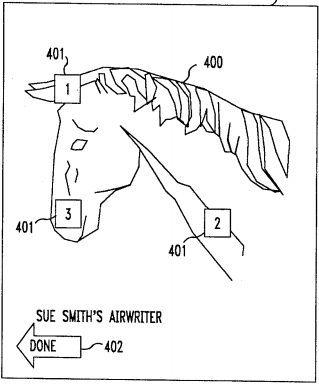
\includegraphics[width=0.30\textwidth]{pics/review/blonder.png}
        \label{fig:blonder}
      }
      \subfigure[DAS \cite{Jermyn}]{
        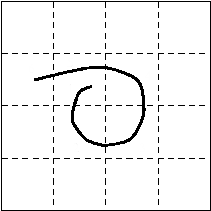
\includegraphics[width=0.30\textwidth]{pics/review/DAS.png}
      \label{fig:DAS}
      }
      \subfigure[BDAS \cite{BDAS}]{
        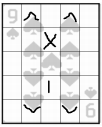
\includegraphics[width=0.30\textwidth]{pics/review/BDAS1.png}
        \label{fig:BDAS}
      }
    \end{figure}

  In 1999, Jermyn et al. \cite{Jermyn} suggested a new graphical password scheme called Draw-a-secret (abbreviated DAS). DAS was the first recall-based graphical password scheme proposed. The motivation for the graphical password scheme was that graphical input devices enables the user to decouple the position of inputs from the temporal order in which they occur, and shows that the decoupling can be used to generate passwords that have a larger and more memorable password space. In order to make a more memorable password, the research group argued that the DAS was more secure than text-based passwords because the users were able to remember longer and more complex passwords. After the DAS scheme was published, Dunphy and Yan \cite{BDAS} added an extra background image to the DAS and named it "Background DAS" (BDAS). The thought behind adding an background to the DAS was to encourage their users to make more complex passwords. Dunphy and Yan believed that the extra image would support the users to remember longer and more complex passwords, and therefore stating that the BDAS was more secure than DAS. Figure \ref{fig:DAS} and Figure \ref{fig:BDAS} are showing images of the DAS and the BDAS respectively.

  In 2000, Dhamija and Perrig \cite{DejaVu}, created a new password scheme called ``Deja Vu''. The password scheme was based on the hash visualization technique \cite{HashVisualization}, a technique that replaces meaningless strings with structured images. The structured images are looking like random art because they are created out of the bits from the meaningless string. Dhamija and Perrig wanted to make a graphical password scheme that solved some of the shortcomings with recall-based authentication like PIN's and text-based passwords. Deja Vu should purely rely on recognition rather than recall, and it should be hard to write down and share the password with others. The randomly generated pictures, based on the hash visualization technique, makes it hard to share the password since the images is hard to recreate but are easy to remember. Instead of writing your own art on a grid, the users are asked to select a sequence of images from a random set of images that are generated by the hash visualization technique. Figure \ref{fig:DejaVu} are showing the Deja Vu where the hash visualization technique are for generating images from random strings looking like random art.

    \begin{figure}[H]
      \centering
      \subfigure[Passfaces \cite{passface}]{
        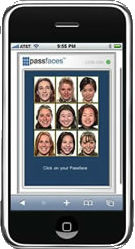
\includegraphics[scale=0.7]{pics/review/Passfaces.jpg}
        \label{fig:Passfaces}
      }
      \subfigure[DejaVu \cite{DejaVu}]{
        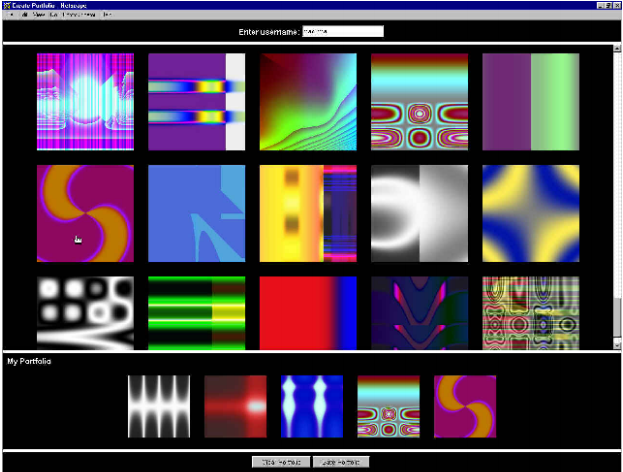
\includegraphics[scale=0.37]{pics/review/DejaVu1.png}
        \label{fig:DejaVu}
      }
    \end{figure}  

  ``Passfaces'' is a graphical password scheme developed by Real User Corporation that was founded in 2000 \cite{passface}. The Passfaces scheme asks the user to first select four images that are a visualization on human faces. The four faces selected represent the password, and the user get authenticated by identifying the four selected faces. The selected faces will be shown together with 8 other faces that is not included in their own selected faces. The scheme exploits the advantage that people are good at recognizing people, so when users choose the human faces they can use the characteristics of the human faces in the process of remembering their password. Passfaces are quite similar to the previous described scheme Deja Vu. The major difference between the schemes are that they are using different association elements in the images, faces and random art. Figure \ref{fig:Passfaces} is showing the PassFaces scheme used on a smartphone. This is one of the few commercial graphical password schemes that are in use. 

  Passdoodle was a new scheme first purposed by Goldberg et al. in 2002 and later studied by Varenhorst in 2004 \cite{PassDoodle,Varenhorst}. The Passdoodle is similar to DAS, but allows users to create a freehand drawing as a password, but uses a more complex matching process without the visible grid. To add variability to the doodles, additional characteristics like color, drawing speed, and number of pen strokes, have been suggested. Figure \ref{fig:doodle} is an example of a freehand drawn doodle.

  In 2004, Davis et al. did a comparison of a light version of ``PassFace'' and a new graphical password scheme called ``Story'' \cite{Davis}. The Story scheme is making the users choosing images to make up a story instead of just recalling a set of faces. Story was created to help users remembering their passwords by making a memorable story of images. In order to pass the authentication, the story had to be recalled in the correct order. To support the memorability, users were instructed to construct a story mentally to connect the everyday images in the set. Figure \ref{fig:story} is an image of Story scheme showing the images of objects used to create a story.

  
  In 2005 Wiedenbeck et al. proposed a graphical password scheme called ``PassPoints'' \cite{Wiedenbeck2} that is an  extension of the Blonder's \cite{Blonder} idea by eliminating the boundaries and allowing arbitrary images to be used. They evaluated their password scheme by testing the scheme for human users. The results showed that PassPoint were a promising scheme with respect to memorability because of the low error rate and low clicking rate. The aim of this study was to get an understanding of how different images affected user performance in authentication with a graphical password scheme. The preliminary result showed suggested that images may support memorability in graphical password schemes. Figure~\ref{fig:passpoints} is an image of the PassPoints scheme.
  \todo{Skrive om dette. Flytte til 4.2?}

    \begin{figure}[H]
      \centering
      \subfigure[Story \cite{Davis}]{
        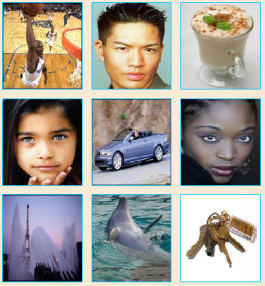
\includegraphics[scale=0.4]{pics/review/story.png}
        \label{fig:story}
      }
      \subfigure[PassPoints \cite{Wiedenbeck2}]{
        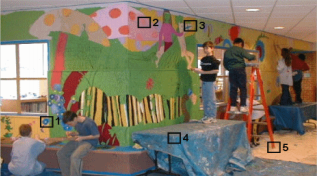
\includegraphics[scale=0.65]{pics/review/passpoint.png}
        \label{fig:passpoints}
      }  
    \end{figure}

  In 2006, a research group wanted to address the problem with graphical passwords and the shoulder surfing problem. They called their password scheme ``Convex Hull Click'' (abbreviated CHC) \cite{Wiedenbeck}. The CHC allows the user to use the scheme in secure and insecure locations because because users do not directly click on the images in the password. This design makes it hard for attackers to perform a shoulder surfing attack. In CHC has a display of small icons. In the authentication process, the user needs to recognize some minimum number of their chosen images, or ``pass-icons'', out of a vast number of randomly placed icons. This step are presented in a sequence, and if the user responds correctly every time, the user pass the authentication. Figure~\ref{fig:chc} is a picture of the CHC password scheme with three selected icons.

    \begin{figure}[H]
      \centering
      \subfigure[Hand-written doodle \cite{Varenhorst}]{
        
\includegraphics[scale=0.55]{pics/review/doodle.png}
        \label{fig:doodle}
      }
      \subfigure[CHC \cite{Wiedenbeck}]{
        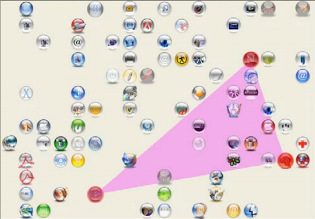
\includegraphics[scale=0.55]{pics/review/CHC.png}
        \label{fig:chc}
      }
    \end{figure}
    
  In 2007, Tao and Adams \cite{Tao} designed the graphical password scheme "Pass-Go". The creation of the scheme was motivated by one of the issues with the DAS scheme where it is difficult to accurately recreate the drawing. "Pass-Go" reduced the issue by using grid intersection points instead of grid cells as used in DAS. The users movements are captured into grid-lines and intersections, eliminating the possibility to reproduce a password where the difference is too high because of the need of precision in DAS. Figure~\ref{fig:passgo} is an image of the Pass-Go grid used.

  Out of the schemes mentioned until now are not widely known nor widely used by users. The first known graphical password scheme that have gained increased attention is the Android Unlock patten. The Android Unlock pattern is a mini version of the ``Pass-Go'' deployed on Google Android smartphones. Rather than entering a four-digit PIN or a text-based password, the user enters a touch-drawn password on a $3\times3$ grid connecting dots forming a password. Figure~\ref{fig:android} is a visualization of the Android Unlock Pattern in use on a smartphone.

    \begin{figure}[H]
      \centering
      \subfigure[Pass-go \cite{Tao}]{
        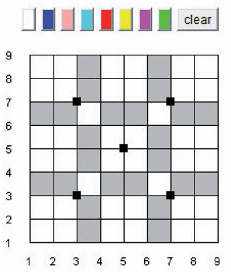
\includegraphics[scale=0.7]{pics/review/passgo2.png}
        \label{fig:passgo}
      }
      \subfigure[Android Unlock Pattern]{
        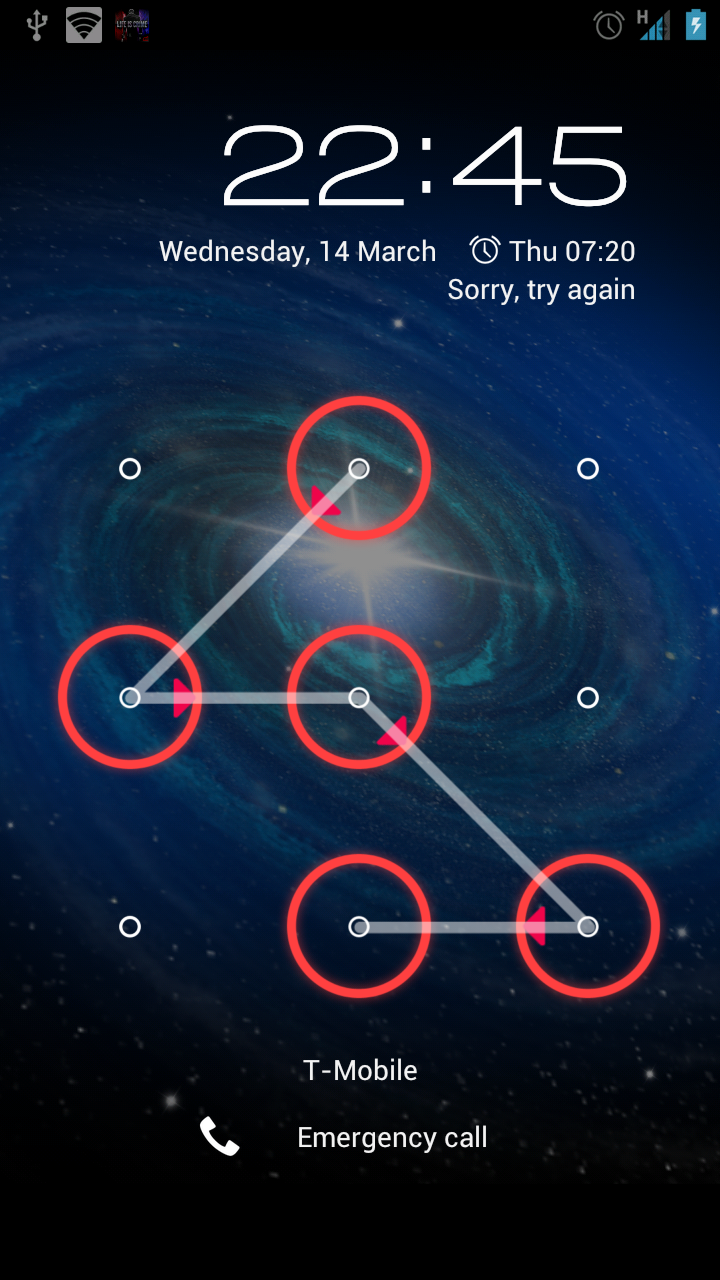
\includegraphics[scale=0.145]{pics/review/patternLock.png}
        \label{fig:android}
      }
    \end{figure}

  Looking at recently published graphical password schemes we will find schemes like GeoPass \cite{GeoPass} and Picassopass \cite{PicassoPass}. Geopass uses a digital map for the authentication phase where the user chooses a particular location as their password. Picassopass is a graphical password scheme presenting a password using a dynamic layered combination of graphical elements. The users can make a story that assists the user in the recognition of the graphical elements. Figure~\ref{fig:geopass} and Figure~\ref{fig:PicassoPass} is the two new proposals for graphical authentication schemes, the Geopass and the Picassopass, respectively. 

    \begin{figure}[H]
      \centering
      \subfigure[GeoPass \cite{GeoPass}]{
        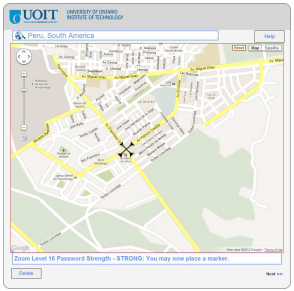
\includegraphics[scale=0.60]{pics/review/geopass.png}
        \label{fig:geopass}
      }
      \subfigure[PicassoPass \cite{PicassoPass}]{
        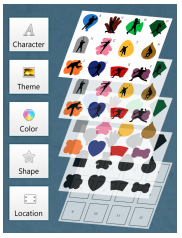
\includegraphics[scale=0.74]{pics/review/picassopass.png}
        \label{fig:PicassoPass}
      }
      \caption{Graphical password schemes}
    \end{figure}
  
	% !TEX root = ../main.tex
\section{Evaluation of Graphical Password Schemes} \label{sec:evaluation}
	
  Authentication with text-based passwords are a traditional approach, but as a cause of limitations of recalling text-based passwords, users choose weaker passwords. Graphical passwords came as an alternative solution for overcoming the limitations of text-based passwords because the graphical memory of humans is particularly well-suited to remember graphical information \cite{DeAngeli}. The problem with many graphical password schemes is that they often promise improved password memorability and thus usability, and at the same time improve the security \cite{Biddle}. The trade-off between usability and security is illustrated in Figure~\ref{fig:usabilitysecurity}. The observed trade-off between usability and security are two aspects important to understand while reviewing the literature of graphical passwords.

  	\begin{figure}[H]
  		\centering
  		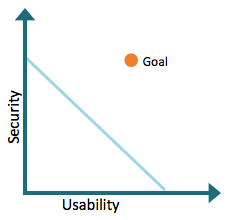
\includegraphics[width=0.40\textwidth]{pics/review/tradeoff.png}
  		\caption{Tradeoff between usability and security}
  		\label{fig:usabilitysecurity}
  	\end{figure}

  \subsection{Usability and Memorability} \label{sec:usability}

    An interesting question is what types of graphical password users find memorable. One of the factors supporting users to remember their selected password relates to the usability of the password scheme. What makes a graphical password having high usability and what is the effect having high usability? This section will look at different graphical password scheme focusing on the usability of the scheme. 

    Deja Vu was one of the graphical password scheme created for being easy to remember, but at the same time being hard to reuse and share as a cause of the random art used. When {\it Deja Vu} first were proposed, the creators conducted a user study showing that 90\% of all participants succeeded the authentication phase using the Deja Vu. On the other side, the creators also revealed that only 70\% managed to pass the authentication process by using text-based passwords and PIN codes \cite{DejaVu}. The difference in success rate is an example that users tend to have a higher success rate remembering graphical password over text-based passwords and PIN codes. 

    One of the first graphical password schemes, {\it DAS} \cite{Jermyn}, offers a theoretical space that are comparable with text-based passwords. Based on cognitive studies of visual information, Oorschot and Thorpe \cite{Thorpe1} investigated the practical password space of the graphical password scheme {\it DAS} \cite{Jermyn}. They found that the password space in practice in {\it DAS} represented an average length of less or equal to the length of 8 on a 5$\times$5 grid. 

    Other researchers have revealed that users tend to draw symmetric images with few pen strokes as well as placing their drawings in the center of the grid. The researchers behind {\it Background Draw A Secret}\cite{BDAS} tried to avoid users placing their drawings in a predictable way and by adding a background image to avoid the predictable behavior. The attached background image resulted in a reduced amount of symmetry within the selected passwords and supported the users to make longer passwords that were similarly memorable as for the {\it DAS}.

    Davis \cite{Davis} did a comparison of the memorability between the graphical password scheme {\it Face} (a light version of the {\it PassFaces}) and {\it Story}. This results reported that users had more difficulties remembering the Story password, resulting in a success rate of  85\%. The low success rate was observed because the users had to remember the correct sequence of the images, instead of remembering the images in an arbitrary sequence. 

    When looking at usability, we can evaluate the graphical layout of a graphical password scheme to see if the visual elements impact the user's choice of passwords. Ullenbeck et al. \cite{Uellenbeck} looked at the Android Unlock patterns and investigated if a change in the graphical layout would impact the security and usability. The original Android Patten Lock uses a sequence of dots connected on a 3$\times$3. Instead of only analyzing the original scheme, they rearranged the points into four separate positions and analyzed patterns created by users for all four rearrangements. The results proved that the unique patterns created doubled by rearranging the points, hence reduced the bias found in the original position of the nodes. Unfortunately did they not only remove some of the bias from the original grid but also introduced new ones. One of the rearrangements was a random approach. Unfortunately, this random arrangement of nodes looked like the mathematical {\it delta} that was people recognized this association element by many of the participants. The random arrangement scored the worst entropy since many of the users selected the same pattern. People are good at recognizing patterns and using association elements. It would not be a surprise if users would find the same results in other rearrangements of the grid if it had a shape similar to other symbols or association elements.

    Wiedenbeck et al. \cite{Wiedenbeck1, Wiedenbeck2, Wiedenbeck3} conducted three lab-based user studies on the graphical password scheme {\it PassPoint}. The results determined that the participants needed an average time of 63 seconds to create their password, and an additional average time of 171 seconds in training time to remember the created password. The login time took an average time between 9 and 19 seconds. The time used highlights the importance of research on usability and memorability when looking at graphical password schemes. The factors making a password scheme having high usability can be determined by looking at the average creation time, time to remember the password, as well as time used in the login phase. 

    It is still a problem that published research on graphical passwords focusing on usability are conducted with a pen and paper approach, raising a question about the validity of the results. One problem may be that many graphical passwords are not implemented, but rather theoretical and visual suggestions. It still a need for further research on graphical passwords in their actual intended environment of use.

	\subsection{Security} \label{sec:security}

    In knowledge-based authentication, e.g. "something you know", we classify attacks into two general categories: guessing and capturing attacks. In a guessing attack, the attackers need to search through the entire password space, often referred to as a brute force attack. A brute force attack validates all possible combinations, making such an attack very time-consuming. If an attacker has some knowledge of the user or the users password habits, the attacker would be able to predict the user's password by avoiding searching through the whole passwords space. Such a reduction in the password space is a reduction in the overall security of the scheme. When managing to reduce the search space, this type of attack is often referred to as a dictionary attack. When talking about capturing attacks, the attackers can directly obtain the passwords by observing the authentication process. One of the known capturing attacks on graphical passwords is shoulder surfing where an attacker are abe to observe a user's password as a cause of a visual presence.

    When selecting a password, many users select a password that connects to them as a person or to something they know. By using this strategy in the process of creating a password, there will be a lower probability of forgetting the password because the password is something you already know. When using such an approach, it is more likely that the person remembers the password, but at the same time helping an attacker to be able to guess the selected password quickly. There is a tradeoff between what is possible to remember and what is secure enough to use; attackers utilize our predictable behavior. A password created using this predictable behavior are called a biased password. A bias is a prejudice in favor of or against one thing, person, or group compared with another, usually in a way that influence a person choice of action. 

    Jermyn et al. \cite{Jermyn} evaluated the security the graphical password scheme {\it DAS}. One of the statements is that the users do not utilize a uniform distribution of the possible passwords by using Klein's study \cite{UnixPasswords} as an argument. The fact that users do not pick passwords uniformly are no itself a sufficient statement to make a guessing attack successful. They try to cover the possibility of an attacker making a successful attack by making their scheme more complex. The results revealed that the generated passwords were significantly harder to crack in practice than textual passwords. The problem with the conducted tests was that they used computer generated passwords that do not achieve the same validity as for using user-selected passwords. They did neither analyze the security of {\it DAS} by including human factors that earlier have been reported to introduce bias in the password selection process.

    Why do users select the passwords they do, and what strategy do they use in the creation process? Davis et al.\cite{Davis} evaluated the security of the graphical password scheme {\it Passfaces}. They found that there was a bias introduced by people's demographics and background. The users tended to choose faces that they liked (their subjective meaning of beauty and attractiveness) and faces they could compare themselves to. The results revealed that if knowing the gender and the race, it would be possible to perform a dictionary attack to guess user-selected passwords in the {\it PassFace} scheme. If the user were male, 10\% of the passwords could easily be guessed on the first or second attempt. Similarly, if the race of the user was known to be Asian and his/her gender is known, then 10\% of the passwords could be guessed within the first six attempts. The result indicated that graphical password being selected by users were heavily biased. The researchers concluded that Passfaces was insecure due to the observed bias in the selection of passwords. 

    Dirik et al. \cite{Dirik} conducted an experiment by modeling users choice in the graphical password scheme {\it PassPoints}. The aim of the study was to test if it was possible to build a dictionary attack based on user's choice in clicking points. In this study, they predefined two different images with a different level of salient points. The researchers reported that they could recover 61\% of a user's selection of clicking points by searching through a smaller password space based on an analysis of collected click-points. The {\it PassPoints} scheme provides user-chosen images, but the aim of this study was to investigate if it was possible to predict users password using a dictionary attack on images having collected data. They observed a slight difference in the two out of three images picked by the researchers. The images including few salient points was being stated as less insecure. Since the {\it PassPoints} scheme enabled user-selected images, the security would rely on the image and clicking points selected by the user, and not the actual scheme itself. The results can not alone state that using {\it PassPoints} are insecure, rather highlighting the importance of considering the human factors in security as it can influence the overall security of the scheme. The same year, an another research group published results on security of the {\it Passpoints} by using two separate research methods  \cite{Thorpe2}. They conducted a user study, as well as a theoretical study image-processing tool, to test if an attack on the {\it PassPoints} scheme was possible. They provided empirical evidence that attractive points, e.g. hot-spots, do exist in images. The results from the most efficient attack were generated by harvesting passwords from users to attack other targets. The probability of the guessing attack showed that 36\% of the passwords selected by users ended up being guessed within $2^{31}$ guesses and 12\% $2^{16}$ guesses. The results from the simulated attack using image-processing were slightly less efficient, but they still managed to prove that an attack on graphical passwords is possible.
    
    In one of the first large-scale studies on the Android Pattern Lock \cite{Uellenbeck} stated that the entropy a pattern is lower than its theoretical entropy. They compared the security offered by the Android Pattern Lock to be less than the security of only three digits randomly assigned PIN for guessing 20\% of all passwords. In the same research, a Markov model based on collected passwords were build. The patterns created was categorized as offensive and defensive patterns as a result of their research design. They set up a game asking all respondents to create a defensive pattern protecting a possible award, as well as creating offensive patterns used for guessing other participants defensive pattern. The results showed that it was possible to guess user's choice in patterns. Within ten guesses, they could guess approximately 4\% of the defensive patterns and approximately 7\% of the offensive patterns. When increasing the number of guesses to 30 attempts, they managed to guess approximately 9\% of the defensive patterns and approximately 19\% of the offensive patterns. If we look further into the Android Unlock Pattern, the scheme has about 400.000 possible valid combinations of patterns. From a theoretical point of view, such theoretical password space are compareable to the security of a 5-digit randomly assigned PIN. The researchers evaluation of user chosen patterns explains that they only have an estimated entropy slightly lower than a 3-digit randomly assigned PINs. Another interesting result is that about 10\% of all users captures less than 190 patterns, while less than 300 patterns capture around 50\% of the whole test population. This result is an indication of the theoretical password space not being a representative number when quantifying the security of a password scheme. We should rather look at the password space in practice, e.g. password that are used and memorized by users.

    Psychology studies have recognized humans superior memory for recognizing and recalling visual information. This observation supports the statement that users can remember more complicated graphical password form a larger password space than an alphanumeric password. Based on this assumption, the attacker needs to build a bigger and more complex dictionary and spend more time to achieve the same success rate as for textual passwords. A clever attacker would narrow down the password space and prioritize guesses to pictures that people are likely to choose. The images that are selected are liable to be the images that users are likely to recall. To understand how an attacker might take advantage of human password choices, psychological studies on humans visual memory are crucial to comprehend.

	% !TEX root = ../main.tex
\section{Psychology and Human Factors}\label{sec:humanfactors}

	In many years, the field of psychology have been important in order to understand how humans interpret and remember information. Psychology studies have recognized that the human brain have a superior memory for recognizing and recalling visual information rather than recognizing and recalling verbal or textual information \cite{DeAngeli}. To be able to go beond the technical part of security, this chapter will include related work on passwords focusing on psychology and the human aspects. Combining research from two different diciplines, computer security and psychology, will give a deeper understnading of passwords at a different level. 

		\begin{wrapfigure}{r}{0.4\textwidth}
      \vspace{-10pt}
      \begin{center}
        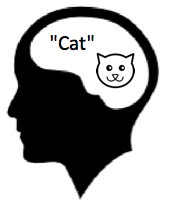
\includegraphics[scale=0.5]{pics/review/dualCoding.png}
      \end{center}
      \vspace{-10pt}
      \caption{Dual-Coding Theory}
      \vspace{-10pt}
      \label{fig:dualcoding}
    \end{wrapfigure}

	One known theory from the world of psychology is the ``dual-coding theory'' \cite{Biddle}. The theory suggests that verbal and non-verbal memory are processed and represented differently in human's mind. Text are verbal information that is represented symbolically, in contrast to non-verbal information like images that are mentally represented in a way that perceived concepts are assigned to a perceived meaning of what is directly observed. Both verbal and non-verbal information can be used when recalling information. For example, say a person have received stimulus of the concept ``cat'', both the image of a cat as well as the word ``cat'' (Figure~\ref{fig:dualcoding}). When a person is asked to recall the concept ``cat'', a person can retrieve the image or the word individually, or both simultaneously. If the word ``cat'' is remembered, the picture of the cat is not lost and can still be retrieved at a later point in time. The ability to code a stimulus in two different ways can increase humans ability to remember, in contrast to only code the stimulus in one way. In the background theory there are described three various categories of graphical passwords according to the memory task involved in remembering and entering the password, e.g. recall, recognition and cued recall.

	When it comes to humans and visual interpretation, studies support the idea that people recall symmetric images better than asymmetric images \cite{Attneave, French}. A particular interesting observation is that mirror symmetry carries a special status I the human memory \cite{Wagemans1}. An understanding of psychological studies on humans visual memory can help to build successful attacks against graphical passwords. If an attacker can successfully use the symmetric properties of graphical password schemes, then the security may be significantly less than if all passwords were equivalent probable.

  Humans do not only tend to choose symmetric passwords, but do also tend to be influenced by the graphical elements in a password scheme. A study on ``PassFace'' \cite{Davis} showed that there was a high bias in the password selection according to a user's gender and race. When they analyzed how each gender chooses their password, the most of the male and female participants chose female faces, and 60-70\% of the user chose a model over a typical female/male. They also looked at the race of the faces, where the results showed that almost all of the participant chose their own race. This research raises the question if it is possible to analyze user's choice in passwords based on the demographics of the user.

  A difference in graphical and text-based password schemes is that graphical passwords can use images with colors that may influence the user's choice in graphical passwords. In a user-study \cite{Thorpe2} on the image-based graphical password scheme ``PassPoints'' managed to see that different images were easier guessed than other pictures. When analyzing different images and visualizations, we can look at studies of gestalt psychology \cite{Wagemans2} that uses the gestalt principles to understand user's interpretation of the picture. One of the images that were the easiest to guess in the user-study was an image with cars in different positions in different colors. A possible explanation could be that humans seek to find a pattern that are easily remembered by using the principles of grouping, similarities of color, and similarity of size in image analysis.

  There are many studies on password based on psychology and human factors, but the graphical passwords schemes being analyzed do not look at the background of the users. Humans are different in terms of their demographics, like gender, age, and culture in their country. Analysis of people choices of graphical password based on user's background have not been looked further into in published research as based on this state of the art research. Since there is a lack of this on graphical password, we will take a look at people choices on text-based passwords based on human properties.

  Password habits may be different across different subpopulation in cause of different background or culture. In 2012 Joseph Bonneau released an analysis of 70 million passwords from Yahoo! \cite{Bonneau2}. The data is analyzed in terms of guessing rate by using a dictionary attack. The collected data contained 328 subpopulations. The results showed that there was no ``good'' populations from the gathered data, but there was a variation in the population. Demographically, the gender had a small effect on the guessing rate, but it showed that age tended to give effect where password strength increases across different age groups. The analysis also showed that language had a significant impact on the password strength where Indonesian-speaking users were among the weakest subpopulations, and in contrast the German and Korean-speaking users provided relatively stronger passwords.

	
	% !TEX root = ../main.tex
\section{Graphical Passwords and Mobile Devices}\label{sec:pwmobiledevices}

	Users are not only dependent on remembering passwords across multiple web pages and systems, but do also need to remember passwords for our small mobile devices. The use of handhold devices, such as smartphones and tablet, has seen tremendous growth in the recent years. The smartphone in general has revived increased attention because of its increased capacity and its variety of use. The first smartphones could access your email, you social network, as well as the basic features of a phone like calling and text messaging. During the past years, the gap between a desktop and a smartphone have become smaller and smaller. People today use their mobile phone for work purposes, mobile banking, online shopping, and other high security tasks. This evolution of the smartphone sets higher standards of security on your smartphone. The smartphone is a handy tool in daily life, but do also contain a lot of sensitive of your private life. Mobile devices can easily be lost or stolen due to it small size, therefore, it is a need to protect the sensitive data from unauthorized access. 
  
  The smartphone have emerged as an excellent platform for graphical passwords because it is easier to input on touchscreen as a contrast to text-based passwords. Graphical passwords on mobile devices seem like a natural fit, as they often require direct manipulation of visual elements. To avoid unwanted access, smartphones offer different locking mechanisms. The history of locking mechanisms was often a solution solely to prevent accidental use, while current mobile phones require protection in order to secure the potentially vast amount of private data that we keep on our smartphones. The situation of our rapid use of mobile phones, as well as it well-suited platform for graphical password, makes authentication on mobile devices an interesting field of study.

  When looking at mobile security it essential to be familiar with the magnitude of mobile phone usage. As of 2014, over 90\% of American adults owns a mobile phone, whereas 58\% of American adults owns a smartphone \cite{MobileUseage}. Another 34\% of the users used their phone mostly to go online instead of using other devices such as a desktop or laptop computer. This is numbers from USA, but it still provides insight information about the use of mobile phones today.

  % Awareness about the sensitivity of the data stored mobile phones
  As stated earlier, smartphone user's tends to store sensitive information on their phones, it is important to understand the relationship between the use of security features and users risk perceptions. One of the key security aspects on mobile phones that are important to understand is why people use or not use locking mechanisms on their smartphone. Engelman et al. \cite{Egelman} published a research paper in cooperation with Google on people's smartphone locking behavior and attitudes towards security of their smartphone data. They observed a strong correlation between the use of security features and risk perceptions. They reported that 33\% of the smartphone users were thinking about the locking mechanisms as too much of a hassle, while 26\% of the user's didn't think that someone would care about the information stored on their phone. Other reported results have covered that the 46.8\% of the participants agreed or fully agreed that unlocking their phone can be annoying. At the same time, 95.5\% of the users somewhat agreed or fully agreed that they liked the idea that their phone was protected \cite{habits3}. The study reported that 29\% did not lock their smartphones \cite{MobileUseage} while another research stated that among 35\% of mobile users do not lock their phone \cite{Bruggen}. The number may vary because of the background and experiences with security while the number remains quite high. This highlights that the users want to be secure, but there might be a trade-off between the time used to unlock the smartphone vs. the security risk.

  % The time used on unlocking the phone
  In terms of security, it is interesting to look at the use of mobile devices and look at the locking habits among users on mobile devices. It is known that services that are rapidly used have weaker password because of the overhead the user needs to spend on typing their password. In 2014 a group of researchers published a field study of smartphone (un)locking behavior \cite{habits3}. Some of the problems with smartphone users tends to be their rapid use of their phone. When the device is rapidly used, it results in much time unlocking their phone between every use. In the study they found that there was a significant overhead in the time used for unlocking their phone, where the users participated in the field study used 2.9\% (9\% in the worst case) of their time unlocking their smartphone.

  It is stated that many users use their smartphones to perform tasks that involve utilization and storage of sensitive data. Smartphones in use today do not require their users to have a locking mechanism on their smartphone. It is well known that users tends to choose the easiest way out and may result in the choice of not having any locking mechanism at all. Based on the outcome of the overhead in time used for unlocking their phone, the result may be to take the easiest way out by ignoring the vulnerability of not using a locking mechanism at all. It has been discovered that over 40\% of the users only used a basic ``slide-to-unlock'' mechanism on their smartphone, as well as over 16\% did not use any locking mechanisms at all \cite{habits3}. This highlights an important bad habit among mobile users. What happens if your mobile is stolen? A loss of a mobile phone is not just the cost of replacing the phone, but also a loss of sensitive data. If the wrong persons find the phone, the sensitive data on the phone may be lost and used for unintended purposes. A 2012 report from Pew Internet estimated that nearly a third of mobile users have had their device stolen or lost \cite{StolenLost}. It is interesting to comparing people's locking behavior towards phones that are stolen or lost. The same report also stated that 12\% of cell owners say that another person have accessed their phone, making the owners feel that their privacy have been exposed to the public.

  Besides losing a physical device, what consequences are users exposed to? One point of attack is to get access to a people's email. If you can grant access to someone's email, you probably can get access to a lot more. In a study reported that all of their interview participants had their email account automatically logged in, as well as 31\% of them did not use any locking mechanism at all \cite{Egelman}. The same research group investigated how much information you could gain from getting access to a person email account. The results showed that both users with or without locking mechanisms found sensitive information in their email account like SSN, Bank Account Number, Email Password and Home Address.

	% !TEX root = ../main.tex
\section{The Android Unlock Pattern}\label{sec:alp}

	One of the most popular smartphones in the market is the Android smartphones. Automatic screen lock is one of the most commonly used protection for unauthorized access on smartphones. Android provides several password mechanisms like PIN code, alphanumeric password, pattern lock, face lock, and slide-to-unlock. Among these screen lock options, the slide-to-unlock mechanism only avoids accidental interaction with the screen. Alphanumeric password and PINs are the must commonly used authentication mechanisms used on smartphones, as well as in other systems requiring authentication. An alphanumeric password are created from all writable characters, while PIN codes only use digits. The newly released face-unlock uses image processing to analyze your face to grant access to your phone. The Android operating system are being known for the graphical password called {\it Pattern Lock} released by {\it Google} in 2008. This graphical password scheme is at this time available on all Android devices, as well provided on other mobile operating systems apart from Apples' mobile operating system, iOS. 

  The {\it Android Pattern Lock} is one of the commonly used screen locks mechanisms on Android devices. For unlocking a device using pattern lock, the user is asked to draw a user-defined sequence of connected dots on a 3$\times$3 grid. Such path is called an lock pattern and is presented in Figure \ref{fig:android}. When creating a pattern, Google has designed several rules for creating a pattern:

  \begin{enumerate}
    \item A pattern needs to be defined by at least 4 dots.
    \item A dot can only be selected once meaning that the maximum number of connected dots are 9 (as defined by the dots in the 3$\times$3 grid).
    \item The pattern will always connect all dots along a path, expect when a dot already has been selected. 
    \item A pattern can go through previously connected dots to connect dots along the same path.
    \item The dots can be connected horizontally, vertically and by the diagonal.
  \end{enumerate}

  The first and second rule only states the minimum and maximum number of connected dots in the pattern. The third rule denotes that if a path is drawn from node 1 to node 3, then the nodes in the path will be $1 \rightarrow 2 \rightarrow 3$ as a cause of rule number three. Rule number four states that you can go through a node that is already in the path, but the node will only be selected once. Such path are called an overlap. Pattern having an overlap are illustrated in Figure \ref{fig:androidrules2} by having chosen the path $5 \rightarrow 3 \rightarrow 7$, where node 5 is not selected twice when going from node 3 to node 7. Figure \ref{fig:androidrules1} illustrates rule number five displaying all nodes that reachable and the valid directions; vertically, horizontally, and diagonally. 

  	%Figure: Illustration of the Android Pattern creation rules
	  \begin{figure}[H]
	  	\centering
	    \subfigure[Reachable nodes from node 1]{
	      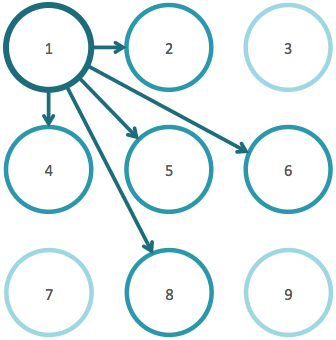
\includegraphics[width=0.4\textwidth]{pics/review/rule1.png}
	      \label{fig:androidrules1}
	    }
	    \hspace{0.8cm}
	    \subfigure[Create a path over a selected node]{
	      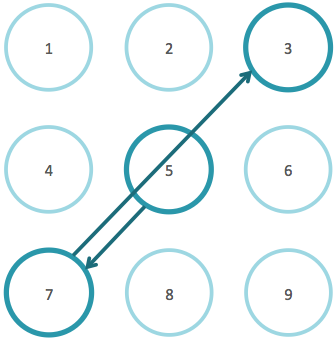
\includegraphics[width=0.4\textwidth]{pics/review/rule2.png}
	      \label{fig:androidrules2}
	    }
	    \caption{Illustration of the Android Pattern creation rules}
	    \label{fig:androidrules}
	  \end{figure}

  In a historical view, the Android Unlock pattern is seen as a new authentication mechanism as opposite to alphanumeric passwords and PIN codes. In a security perspective, the pattern has a total of 389,112 valid patterns using a $3\times3$ grid. Comparing the Android Lock Pattern with PIN codes, having 10.000 possible codes, the Android Lock Pattern seems to be more secure. Compared to an alphanumeric password, the number of combinations depends on the number of characters included. When looking at published research, users are capable of remembering passwords with an average length of 7 to 8 characters. As introduced, the Android unlock pattern is a more suitable form of authentication for mobile devices due to its interactive and graphical form that suits small touch screens. When using an alphanumeric password on a smartphone, a virtual keyboard are used typing the password, making it less suitable for mobile devices because of the size. Smartphones are being used in various situations during a day, making it desirable to use an authentication mechanism that is quick to type and easy to remember, avoid spending the time unlocking the smartphone. It is no secret that an alphanumeric password with its extensive password space would be more secure if users created long passwords. However, this is not the reality because mobile devices do are not suitable for typing long passwords on the virtual keyboard. To further explore the security and usability of the Android unlock pattern,  we will take a look at published research to get an overview.

  	%Table: Number of pattern combinations
	  \begin{table}[H]
	    \centering
	    \begin{tabular}{| l | l |}
	      \hline
	      {\bf \# Length} & {\bf \# Valid combinations} \\ \hline
	      4 & 1624 \\
	      5 & 7152 \\
	      6 & 26,016 \\
	      7 & 72,912 \\
	      8 & 140,704 \\
	      9 & 140,704 \\ \hline
	      Total & 389,112\\ \hline
	    \end{tabular}
	    \caption{Number of pattern combinations}
	    \label{tab:combinations}
	  \end{table}

  As stated, the Android Pattern Lock has 389,112 valid patterns, according to the listed rules. But is this number as secure as it sounds? When looking at the security of a password scheme it can evaluated according to total valid combinations, e.g. the password space or the passwords that statistically are likely of being chosen. The passwords that statistically are likely of being chosen refers to the password space in practice. Table \ref{tab:combinations} summarizes the total number of valid combinations based on the pattern length \cite{Sun}. An another way of look at the security of the a pattern is to measure the pattern strength. A research paper investigated the use of password meter for measuring the strength of a pattern. Their hypothesis was that the utilization of a password meter was providing more secure user-selected patterns. They stated that there often tended to choose a short and easily guessed pattern due to memorability. A password meter is often shown as a colored bar that is often used as an indication of the strength of a password. The research group used a mathematical equation (\ref{eq:patternstrength}) for calculating the strength of Android pattern locks. 

    \begin{equation}\label{eq:patternstrength}
      PS_{P} = S_{P} \times log_{2}(L_{P} + I_{P} + O_{P})
    \end{equation}

  $PS_{p}$ is the strength score of pattern P. $S_{P}$, $L_{P}$, $I_{P}$, and $O_{P}$ are the number of connected nodes, the physical length, the number of intersections, and the number of overlaps of P, respectively. Using Equation \ref{eq:patternstrength} on all valid patterns gives a score from 6.340 to 46.807. The formula was being utilized by Sun et al. \cite{Sun} in their research on Android patterns and password meters. They look at pattern strength in a different way other than just calculating the complexity of a pattern by its length. Calculating password complexity by length seems as a naive approach, making this way more realistic using all the rules of the Android pattern in the equation. When looking at the different characteristics and strength of a pattern used in Equation \ref{eq:patternstrength}, Sun et al. maked distribution graphs of the different characteristics and the strength (Figure \ref{fig:patterngraph}).

  	%Figure: The distribution of the pattern characteristics and strength
    \begin{figure}[H]
      \centering
      \subfigure[Pattern physical length]{
        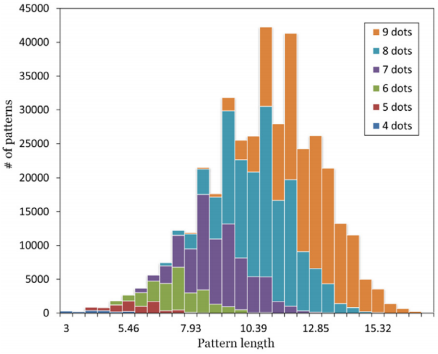
\includegraphics[scale=0.35]{pics/review/patterngraph1}
        \label{fig:patterngraph1}
      }
      \subfigure[Pattern intersections]{
        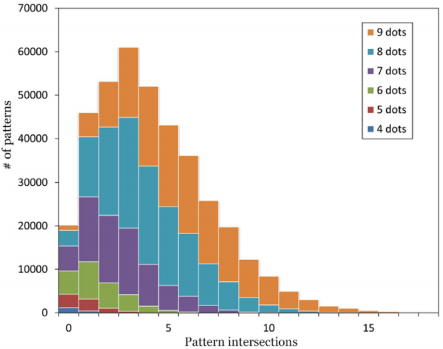
\includegraphics[scale=0.35]{pics/review/patterngraph2}
        \label{fig:patterngraph2}
      }
      \subfigure[Pattern overlaps]{
        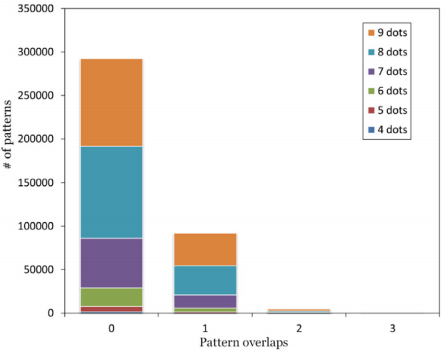
\includegraphics[scale=0.35]{pics/review/patterngraph3}
        \label{fig:patterngraph3}
      }
      \subfigure[Pattern strength]{
        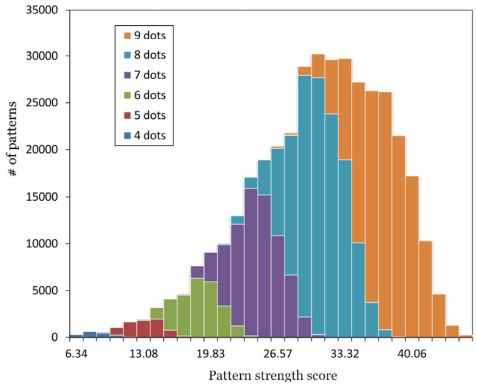
\includegraphics[scale=0.35]{pics/review/patterngraph4}
        \label{fig:patterngraph4}
      }
      \caption{The distribution of the pattern characteristics and strength \cite{Sun}}
      \label{fig:patterngraph}
    \end{figure}

  Sun et al. \cite{Sun} created two different visualizations of a password meter, one looking like a progress bar (Type 1), and one indicating a percent of the strength (Type 2). They recruited 81 participants for a survey testing the strength of user-created patterns. They divided the participants into three separate groups; no password meter (Group A),  password meter type 1 (Group B), and password meter type 2 (Group C). The survey randomly assigned the participants to the separate groups. The result revealed that the strength of the created patterns in group B and C had a higher complexity and strength but had a higher error rate when retyping the pattern. As a researcher explained, users are typically more security conscious when they are aware of the need for such behavior \cite{Sasse}. The error rate points to the problems with passwords and security in general. A long and complicated password are harder to guess but are not likely to be selected due to memorability issues. Also, a problem with the Android Pattern is that the pattern is being frequently used as it is provided to grant access to the smartphone in all kind of situations. The results from the survey states that the input convince was the reason that caused the highest number of participants in the user study not selecting a pattern with a high complexity and strength. A pattern containing more dots takes a longer time to type. When looking at patterns containing intersections and overlaps, there is a high chance of accidentally hitting a wrong dot when drawing a pattern. Such an error are causing the user to redraw the pattern, hence spending more time passing the authentication process. The conclusion is that the time used to type the pattern are as crucial as the time used to memorize the pattern when looking at the users choice in patterns.

  The pattern strength meter gives a score of the visual complexity of a pattern. The benefit of looking at the visual complexity instead of only looking at the length can be seen in Figure \ref{fig:patternstrengthexamples}. When looking at Figure \ref{fig:strength1}, \ref{fig:strength2}, and \ref{fig:strength3}, they have all have the maximum length, but at the same time having a different pattern strength, e.g. a difference in visual complexity. Figure \ref{fig:strength7}, \ref{fig:strength8}, and \ref{fig:strength9} have all the minimum length of four dots, but they still have a difference in the measured strength. The visual complexity is one of the extra security dimensions to study when working with graphical passwords. The pattern itself is just a sequence of numbers, but the order of the sequence can make a big difference in visual complexity, and can be important when wanting to avoid known attacks like shoulder surfing. 

  When looking at user-selected passwords, studies tell that many users are using graphical shapes to support memory \cite{Weiss}. Sun et al. \cite{Sun} analyzed collected Android Lock Patterns and found empirical evidence that some users tended to use patterns which looked like letters or numbers. They found patterns looking like the letters and numbers C, L, N, Z, 2, and 7 that easily can be created on a 3$\times$3 grid. Such a strategy for enhancing memorability by using association elements, e.g something that the user are familiar with, are used in other password schemes. The use of association elements is known to used in PIN codes and alphanumeric passwords where names, objects, dates are used to remember the password instead of a visual representation of a letter or number.

  Android Unlock pattern have been shown to have biases when being user-chosen. A research group did one of the first large-scale user study on the security of the Android Unlock Patterns in order to quantify the security of the {\it Android Pattern Lock} \cite{Uellenbeck}. They analyzed the biases introduced in the pattern making process and added changes to the scheme in order to avoid the known biases in the password scheme. The researchers found that there was a high bias in the pattern selection process, e.g. the upper left corner and three-point long straight lines are likely being selected. If user-chosen patterns were being uniformly chosen, the probability of starting in at any point should be 11\%. The results revealed that there was a strong bias towards the starting point in the corners. If the points were uniformly chosen, the probability for all four corners should be 44\%, but the results showed that the probability is close to 75\% in their pen-and-paper study. In contrast, the center point, the right, the upper, and the lower center points only got a probability of 14\% to be selected. Other results from the pen-and-paper study found that the average pattern length was 5.63 with a standard deviation of 1.5. As stated earlier, users tend to take the easiest way out, making users choose short patterns that are easy to remember and type. Looking at the selection of starting node, 43\% in the user study, and 38\% in the pen-and-paper study selected the upper-left corner as their starting node. This is supporting the researchers claim that users tend to choose less secure patterns ``in the wild'' than a theoretical evaluation of a password scheme.

  What is causing the biases observed in the Android Pattern Lock? The next chapter will introduce a research design for collecting Android Pattern Locks for further analysis focusing on human factors.

  \clearpage

    \begin{figure}[H]
      \centering
      \vspace{1.5cm}
      \subfigure[Sequence: 147852369, \newline Strength: 27.00]{
        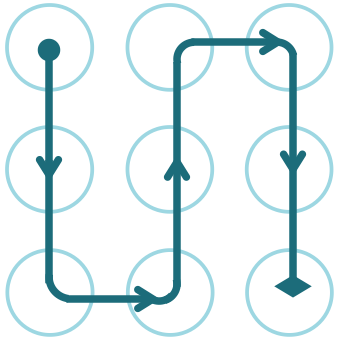
\includegraphics[width=0.27\textwidth]{pics/experiment/strengthpattern2.png}
        \label{fig:strength1}
        \hspace{0.6cm}
      }
      \subfigure[Sequence:213546879, \newline Strength: 36.655]{
        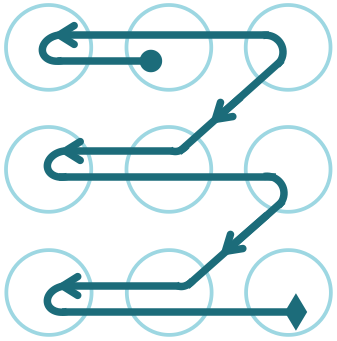
\includegraphics[width=0.27\textwidth]{pics/experiment/strengthpattern3.png}
        \label{fig:strength2}
        \hspace{0.6cm}
      }
      \subfigure[Sequence: 591827346, \newline Strength: 46.807]{
        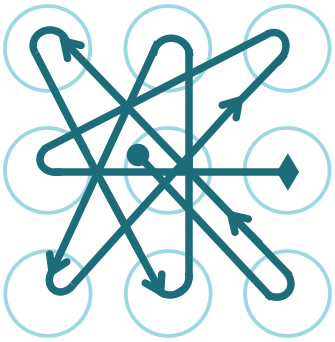
\includegraphics[width=0.27\textwidth]{pics/experiment/strengthpattern1.png}
        \label{fig:strength3}
      }
      \vspace{0.5cm}

      \subfigure[Sequence: 968752, \newline Strength: 15.259]{
        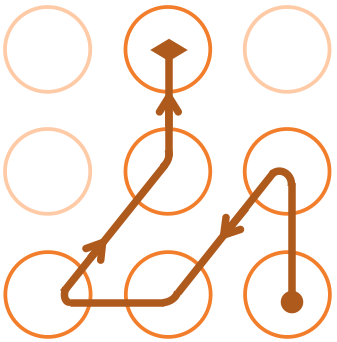
\includegraphics[width=0.27\textwidth]{pics/experiment/strengthpattern7.png}
        \label{fig:strength4}
        \hspace{0.6cm}
      }
      \subfigure[Sequence: 1269853, \newline Strength: 20.781]{
        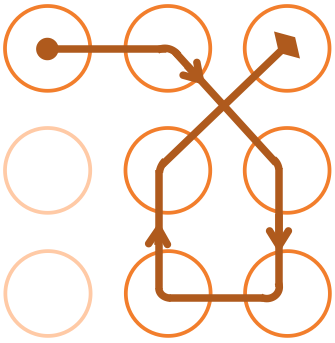
\includegraphics[width=0.27\textwidth]{pics/experiment/strengthpattern8.png}
        \label{fig:strength5}
        \hspace{0.6cm}
      }
      \subfigure[Sequence: 36578249, \newline Strength: 30.512]{
        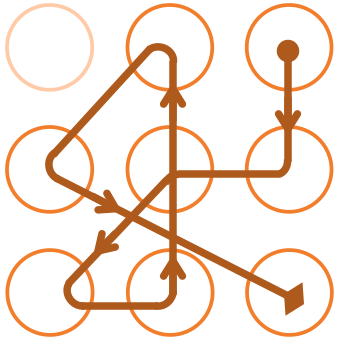
\includegraphics[width=0.27\textwidth]{pics/experiment/strengthpattern9.png}
        \label{fig:strength6}
      }
      
      \vspace{0.5cm}

      \subfigure[Sequence: 1478, \newline Strength: 6.339]{
        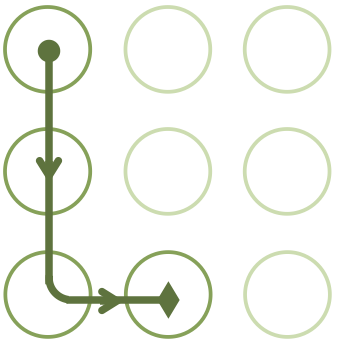
\includegraphics[width=0.27\textwidth]{pics/experiment/strengthpattern4.png}
        \label{fig:strength7}
        \hspace{0.6cm}
      }
      \subfigure[Sequence: 5968, \newline Strength: 9.086]{
        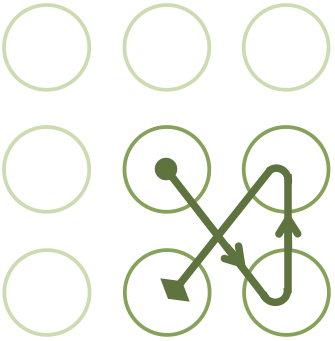
\includegraphics[width=0.27\textwidth]{pics/experiment/strengthpattern5.png}
        \label{fig:strength8}
        \hspace{0.6cm}
      }
      \subfigure[Sequence: 4927, \newline Strength: 11.786]{
        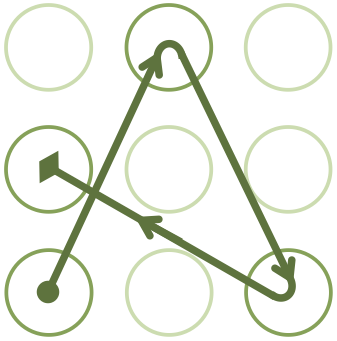
\includegraphics[width=0.27\textwidth]{pics/experiment/strengthpattern6.png}
        \label{fig:strength9}
      }

      \vspace{0.5cm}
      \caption{Examples of patterns with different length and strength}
      \label{fig:patternstrengthexamples}
    \end{figure}


	% !TEX root = ../main.tex
\chapter{Data Collection}\label{chap:experiment}
  
  \clearpage
  \section{Research Strategy}\label{sec:researchStrategy}
    This section will provide information about the chosen research strategy. A research strategy is being considered as the selected strategy for being able to answer the main research goals; the hypotheses and the research questions. Briony J. Oates \cite{empiriske} presents six different research strategies: survey, experiment, design and creation, case study, action research, and ethnography. This section will not go further in describing the difference between the six strategies, but rather explain the choice of research strategy. The detailed work behind the choice in research design was carried out in preliminary work beforehand of this thesis \cite{prosjektoppgave}.

    The selected research strategy for this dissertation is a survey. The idea of a survey is that it will obtain some kind of data from a large group of people or events, in a standardized and systematic way \cite{empiriske}. The survey is chosen due to the amount of data needed for the analysis, as well as the lack of time for choosing other approaches, like interviews and other observation techniques. There are different ways of creating a survey, for example, pen-and-paper or using an online survey. For this research, an online survey is selected for several reasons. First, a pen-and-paper survey is too time-consuming to perform and are not scalable for international data collection. It is also desired to keep responses anonymous due to the topic of research. The form of administration is, therefore, self-administered as there is no one present when the respondent answers the survey. More information about the sampling technique is described in section \ref{sec:samplingTechnique}.

    In the preliminary work, wireframes were created as a draft of the survey. These wireframes can be found in Appendix \ref{ap:wireframes}. Chapter \ref{sec:survey} will have a final implemented version giving a more detailed description of the survey.

  \section{Sampling Technique}\label{sec:samplingTechnique}
    The {\it sampling frame} is a list of the whole population of people that could be included in the survey. When looking at the sample of this study, there is not possible to make a limited sampling frame that can be summered in a list. The population of the sample frame is considered as all people with a smartphone because this research looks at people's choice of Graphical Password, in particular the Android Lock Patterns that is a mobile authentication scheme.

    When conducting a survey, it needs to be decided how to select people from the sampling frame. There are two different ways of doing sampling: probability sampling and non-probability sampling \cite{empiriske}. Probability sampling means that the sample has been chosen because the researcher believes that there is a high probability that the sample of respondents selected is representative for the overall population being studied. Non-probability sampling means that the researcher does not know whether the sample of people is the overall population.

    Because of the broad sampling frame it would be feasible to use non-probability sampling for this research. When using non-probability sampling, we make a decision that it is not practicable to describe a representative sample because there is too much uncertainty about the respondents that will voluntary answer the questionnaire. When choosing a non-probability sampling, we need to select an {\it sampling technique}. The possible sampling techniques we can choose from is purposive sampling, snowball sampling, self-selection sampling, and convenience sampling \cite{empiriske}. The {\it purposive sampling technique} requires the researcher deliberately to choose people that are likely to produce valuable data to meet the purpose of the research. This requirement would not be a good technique because I am not able to pick who would participate, as well as the data collection need to be performed worldwide. A Purposive sampling technique would maybe provide a more uniform collection of people, but it is hard to control respondents when the survey is distributed over the Internet.
    The {\it snowball sampling technique} utilize the network from one person of the sample frame, and then collects new names from that person. The need for directly communicate with respondents is not possible for me as a researcher. {First}, I have no contact with the respondents. {Second}, the respondents, should remain anonymous when answering the questionnaire, as well as there should be possible to track the information back to the respondent. When using the {\it convenience sampling technique}, the researcher only selects respondents who are convenient for them, because they are easy to reach or willing to help.

    When doing {\it self-selection sampling}, the researcher advertises their interest in a particular topic and their need for respondents and collect data from anyone who are willing to participate. The self-selection sampling strategy looks like an excellent fit for the research. The survey needs to be distributed over the Internet, and the self-selection strategy will support this choice. People who select themselves for research often do so because they have strong feeling for the subject, or that the research can bring them a personal benefit. A self-selection sampling technique may also reduce the bias that can be introduced when the researcher hand-picks the respondents. With the self-selection sampling strategy allows all interested peoples with a smartphone to participate in the research. The self-selection is a useful technique when directly contact is not achievable. The self-selection sampling remains the technique that are looking as the best fit for this research.

  \section{Review of Human Properties}\label{sec:reviewofproperties} 

      When using an online survey, the human properties must be carefully selected. {\it First}, when a survey is distributed on the Internet there is no way back, and we need to be sure that the chosen questions will provide sufficiently and relevant data for answering the hypothesis. {\it Second}, we need to review all human properties and only select a suited number of them. A too long survey may result in a small number of responses because the time needed to complete the survey if all the properties is included. {\it Third}, some of the properties may not have a suitable grouping of answers, and may be challenging to include in a survey that needs to be replied to on a mobile device. If such a property is included, it needs to provide irreplaceable and valuable information for the analysis. The survey should try to avoid time-consuming and complicated questions if possible. This section will provide a detailed review of the human properties.

      \subsection*{Age and Gender} 
      A group of people within a particular group of age may have different risk awareness. A person with an age of 30-40 years and a person younger than 20 years may have different concerns with security. A person of age between 30-40 may use their phone to perform a task with requiring high security, like tasks related for work purposes. A person with an age below 20 may not have the same security awareness because of the different use of mobile devices, as well as experience. Age is also interesting demographic information that can be used to group the respondents into distinct subgroups. When looking at gender, psychological studies have reported that males are more likely to take risks than females \cite{Byrnes}. In the literature review, there were no results found related to gender and risk awareness. However, researchers have found bias in the password selection process of {\it PassFace} when looking at gender.

      \subsection*{Language preference}
      By asking the respondent about their language preference it can be used to check whether the alphabet a respondent use impacts their choice in lock pattern. For example, Chinese words are written in a different way then people using the Latin alphabet. In the Android Unlock Patterns, people are able to create patterns looking the same as the letters \texttt{'L'}, \texttt{'M'}, and \texttt{'O'}. The Figure~\ref{fig:letters2} there is an illustration the letters that are possible to select a lock pattern. The same possibility could be found in languages using a different alphabet than the Latin. When looking at PIN codes, there are certain numbers that have a different meaning than only its numeric value. In China, people are associating certain words with numbers or things based on the similarities of sound. For example, the number eight is considered as a lucky number because it is pronounced "ba", which sounds like the Chinese word for prosperity \cite{ChineseChatCodes}. Other numbers like 4 and 775 are pronounced in the same way as "death" and "Kiss me", respectively. Looking at the selection of PIN codes based on people's language, people tend to choose PIN codes that they can associate to a number of special meanings. Examples of this behavior are PIN selection corresponding to date of birth. 

        \begin{figure}[H]
          \centering
          \subfigure[The letter L]{
            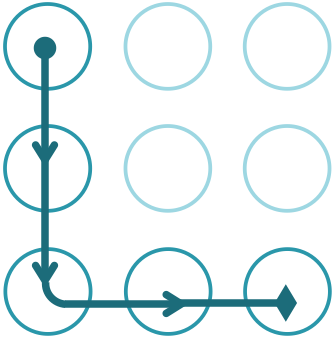
\includegraphics[width=0.25\textwidth]{pics/letters/bokstavenL.png}
          }
          \vspace{0.2cm}
          \subfigure[The letter M]{
            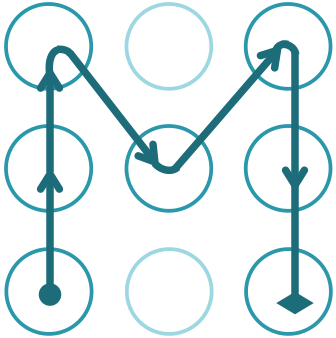
\includegraphics[width=0.25\textwidth]{pics/letters/bokstavenM.png}
          }
          \vspace{0.2cm}
          \subfigure[The letter O]{
            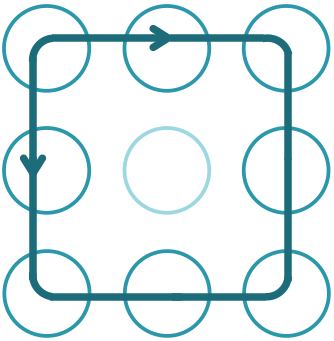
\includegraphics[width=0.25\textwidth]{pics/letters/bokstavenO.png}
          }
          \caption{Patterns corresponding to letters}
          \label{fig:letters2}
        \end{figure}

      \subsection*{Handedness}
      An interesting property of humans is the fact that people write with either left or right hand (and sometimes both). Handedness can influence the way a person are holding a mobile phone, and may impact their choice of lock pattern. In the literature review, it was not found any studies that reported results of people choices in patterns based on handedness. Published research \cite{Uellenbeck} found that over 40\% of the participants in their study started their Android pattern by beginning in the upper-left corner, but did not record the hand used when collecting the patterns. A question to be answered is whether a left-handed person using the left hand while interacting with the screen increases the probability for starting in the upper right corner. Figure \ref{fig:handedness} illustrates handedness and likely starting point as a hypothesis, where the percentages attached to the nodes are indicating the probability for starting in the node. The right part of Figure \ref{fig:handedness} are collected from the research by Uellenbeck \cite{Uellenbeck} while the numbers on left part are only hypothetical numbers. Since it is more likely that people are right-handed, are we able to mirror the results in the right figure for left-handed people? My hypothesis as stated earlier is that people that are left-handed are more likely to start in the upper right corner, while people that are right-handed are more likely to start in the upper left corner.

        \begin{figure}[H]
          \centering
          \subfigure{
            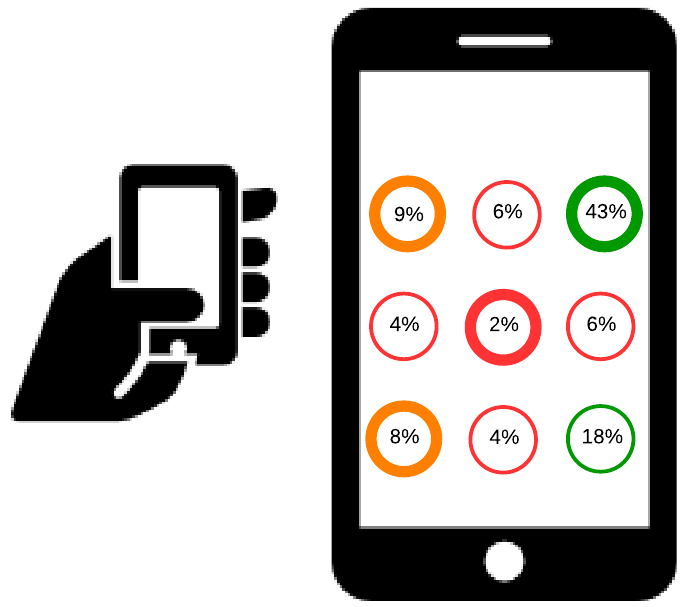
\includegraphics[scale=0.2]{pics/review/handednessLeft.png}
          }
          \subfigure{
            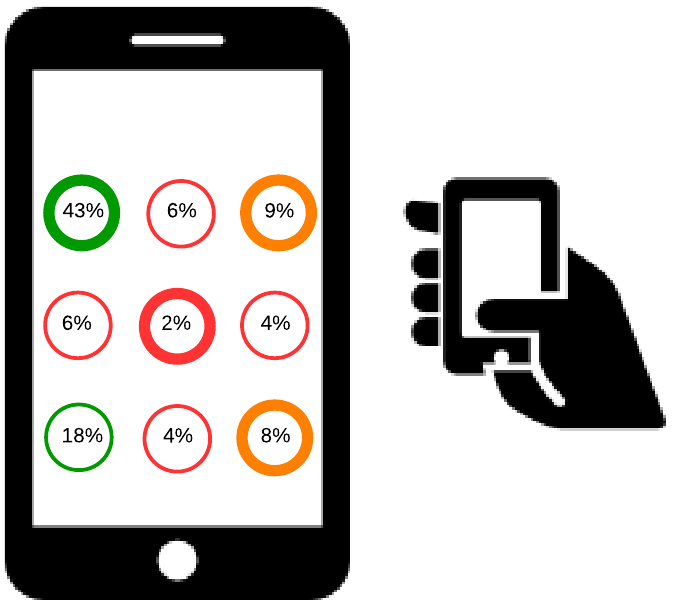
\includegraphics[scale=0.2]{pics/review/handednessRight.png}
          }
          \caption[Likely chosen initial starting point and handedness]{Likely chosen initial starting point \cite{Uellenbeck} and handedness}
          \label{fig:handedness}
        \end{figure}

      \subsection*{Nationality} 
      The nationality of users is often used in research on graphical passwords. When asking a person about their PIN code, a nationality can be used to find likely numbers to appear because some cultures associates a number with a historical or religious event. In a research on the {\it PassFace}, the nationality of the participants was proven to be valuable because people tended to choose faces from the same race and nationality. In this research, it is uncertain how much this information will help to prove any connection between nationality and users choice in patterns. Properties like language preference and reading/writing orientation look more promising for this research. However, the nationality is a data property that are useful when getting an overview of the population.

      \subsection*{Reading and writing orientation}
      In different cultures, there is a difference in the reading and writing orientation. Cultures of Europe and America usually write and read horizontally from left to right, but there are other cultures that do otherwise. Figure \ref{fig:orientation} illustrates three different ways of reading and writing. Traditionally, Chinese, Japanese, and Korean are writing text vertically in columns from top to bottom, from right to left. Another writing orientation is horizontal from right to left used in Arabic speaking countries. Today, the vertical orientation from top to bottom is often in a horizontal way due to the influence of English and the increased computerized typesetting, but both ways are still in use. There is research that have reported that the writing orientation are affecting the visual attention and memory \cite{Chan}. They found that the reading orientation affected the way a person would memorize objects. They reported that English and Chinese speakers tended to remember an image that appeared in the top, left-hand side of the screen. The Taiwanese speakers in the study tended to remember images on the opposite side of the screen, the images on the upper-right side of the screen. An interesting aspect of the reading and writing orientation is to see if people from different cultures are choosing different patterns due to their writing orientation. 

        \begin{figure}[H]
          \centering
          \subfigure[Left-to-right]{
            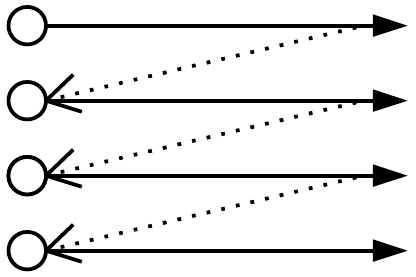
\includegraphics[scale=0.25]{pics/review/leftright.png}
          }
          \subfigure[Right-to-left]{
            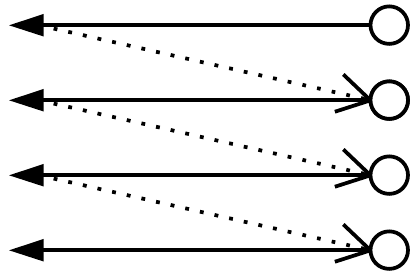
\includegraphics[scale=0.25]{pics/review/rightleft.png}
          }
          \subfigure[Top-to-bottom, left-to-right]{
            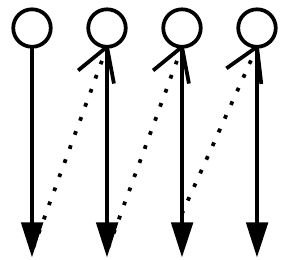
\includegraphics[scale=0.27]{pics/review/topbottom.png}
          }
          \caption{Reading and writing orientation}
          \label{fig:orientation}
        \end{figure}

      \subsection*{Profession and Occupation}
      The current profession of a person may say something about persons knowledge and background. When looking at profession, a person with a profession in IT may be more certain of the security aspects than people in other professions. It may cause bias in the data if people with enough knowledge of security overcompensate their choice of lock pattern because they want to prove their knowledge. Occupation is valuable information due to the knowledge level of the respondents. The occupation of the a respondent is simply if a person is a student, employed, not employed or retired.

      \subsection*{Finger, handsize, and screensize}
      When looking at the finger used when creating the pattern, it impacts the reachable areas on the smartphone. When interacting with a smartphone, the most common way is to either use the thumb or the forefinger. When combining this property with the screen size and the size of the hand, we might be able to predict the selection of patterns by eliminating areas that are harder to reach. In a book called {\it Designing Mobile Interfaces} \cite{Hoober}, they used an expression called the {\it thumb zone}. The Thumb Zone is the most comfortable area for a person to touch when holding a smartphone using one hand. Figure~\ref{fig:thumbZone} is showing the thumb zone where the green area is where the thumb can easily access. The orange and the red areas are part of the screen that is harder to reach. The thump zone can be used when looking at users choice of patterns a pattern that are easy to type can be more likely of being created. Smartphones today tends to get bigger and bigger in size. An interesting analysis could be done by looking at user's choice in patterns based on the size of their hands and size of the screen. By looking at a situation where a person with a small hand is interacting with a big screen, it may be hard to reach certain areas of the screen when holding the smartphone in one hand. Maybe a right-handed person with a small hand interacting with a large screen will not be able to reach the upper left corner? The situation are illustrated in Figure~\ref{fig:reachablePoints}.

        \begin{figure}[H]
          \centering
          \subfigure[Reachable points on screen]{
            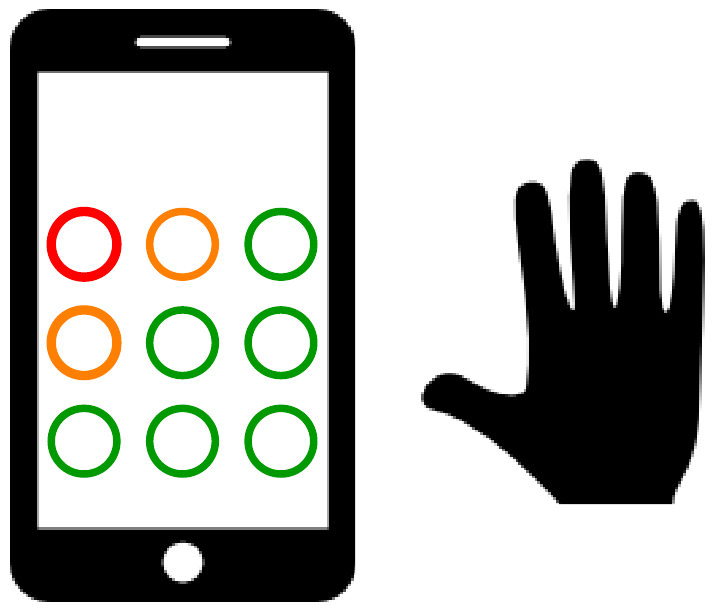
\includegraphics[scale=0.22]{pics/review/screenHand.png}
            \label{fig:reachablePoints}
          }
          \hspace{1.0cm}
          \subfigure[The thumb zone]{
            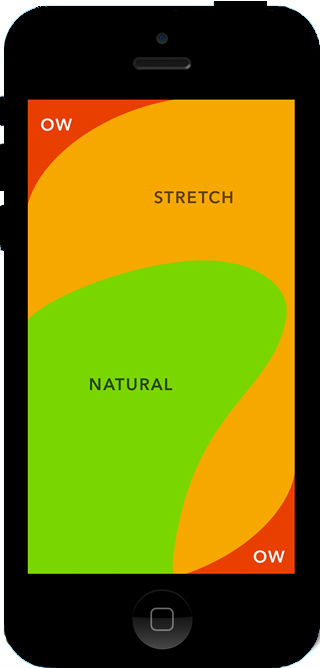
\includegraphics[scale=0.20]{pics/review/mobileScreen.jpg}
            \label{fig:thumbZone}
          }
        \end{figure}

      % \subsection*{Selection of Human Properties}
      % Based on the human properties review, not all of them have the same potential for being included in the data collection. First, the human properties have to have potential for getting interesting results. Second, the property are collected from a mobile survey, meaning that it have to be possible to collect the information based on a question. 

      % The handsize of a person and the finger used when creating the pattern is an interesting combination. The screensize is not directly a human property, but is included because is impacts the reachable areas on a mobile screen based corresponding to the handsize. The finger used can be directly asked for in the survey, while screensize and handsize are categorized as being subjective. When collecting handsize and screensize, the data collected needs to be further evaluated for its validity.

      % Nationality and reading and writing orientation are two properties closely related, and both properties are further included. Language preference will not be included in the survey as there are many languages. 

      % Profession and occupation is not easy to ask for as the number of professions are high as well as depending on where a person live. It is not easy to obtain any significant result as there are too many professions. Instead of collecting all professions, the experience with IT and security are included as it is relevant to the topic of research. 

      % Age and gender are information that are characteristic to have when analysing subgroups, as well as getting an overview of the entire population. 
      % Handedness 
  
  \section{Calculating the Sample Size} \label{sec:samplesize}

    It is essential to determine an appropriate sample size to be able to make any conclusions with the data. When a sample size is too big, it will lead to an unnecessary waste of time in this study due to the time frame of the thesis. On the other hand, if the sample size is too small, the results can not be considered to be used for statistical tests, and it might not be possible to come up with a reliable conclusion.

    When using known formulas for calculating the sample size, you need to know the population size, preferred margin of error, desired confidence interval, and the percentage of the population that is likely to answer. In this study, these parameters are hard to determine because of the non-probability sampling technique that are being selected for this study. For example, the targeted population size is hard to estimate because it includes all people with a smartphone worldwide. Because of the uncertainty connected to the sampling technique, there do not exist a known formula for calculating the sample size. We are not able to calculate the sample size by a known formula, but the sample size still needs to be decided based on my subjective meaning. The sample size is determined by what is achievable with the time frame available, as well as what I as a researcher think of as a good enough sample to ensure sufficient data for getting any results.

    The greater the accuracy required by my claim that my sample size represent the whole population adequately; the larger your sample size needs to be. Statisticians have produced tables that correlate population size against the sample size for the required level of confidence and accuracy. Table~\ref{tab:sampleSize} is a recommended sample size for using a survey (using 95\% confidence interval and +/- 3\% accuracy range) estimated by the targeted population size \cite{empiriske}. As stated in Table~\ref{tab:sampleSize}, the sample size does not increase at the same rate as the target population. When looking at all people that owns a mobile phone worldwide, we can argue that the targeted population size is greater than 1,000,000, and we, therefore, need a sample size of at least 1000. It would be desirable to get a sample size bigger than 1000, but due to the time frame of this research, a sample size of 1000 should me achieved.

      \begin{table}[H]
        \centering
        \begin{tabular}{| p{5cm} | p{5cm} |}
          \hline
          {\bf Target Population Size} & {\bf Required sample size} \\ \hline
          50 & 47 \\
          5000 & 760 \\ 
          100,000 & 888 \\
          900,000 & 895 \\ 
          $>$1,000,000 & 1000+ \\ \hline
        \end{tabular}
        \caption{Target population and sample size \cite{empiriske}}
        \label{tab:sampleSize}
      \end{table}

    Since the sampling size is quite high, and the survey is being distributed with a self-selection sampling strategy over the Internet, it is still important to provide some level of control of the respondents. Using a self-selection sampling technique implies that there is no control of who will answer the survey, hence likely that some subgroups will have a higher representation that others. In a situation where lacking respondents from a subgroup, it should be recruited more participants from the subgroup. However, when using such a strategy, it might introduce some bias because I would then influence the sample. Section \ref{sec:response} will look at some strategies for responses from different subgroups that may be underrepresented when using a self-selection sampling technique. 

  \section{Response Rate and Non-responses} \label{sec:response}

    The survey is distributed over the internet, making it difficult to maintain control over how many people are willing to respond and how many people from different subgroups that are reachable. To be able to achieve the amount of data needed for an analysis, a strategy are need if a subgroup are being underrepresented in the sample. Below, there are listed a strategy for collecting data from the different subgroups. The strategies are being included as a cause of some subgroups might being less willing to respond, or harder to reach, because they are outside the network of the people involved in this research.

    {\bf People with age of 60 or higher:} 
    People with the age over 60 may not own a smartphone or may be hard to reach for other reasons. It would be beneficial to find networks where containing a high representation of people with an age of 60 or higher. In Norway, there is a network called "Seniorweb." There is also a magazine called ``vi over 60''  for senior citizens with members with an age over 60. Both networks are possible to contact if there is a lack of respondents from this subgroup.

    {\bf People with a different field of interest than IT and security:} 
    The network of the people involved in this research is being overrepresented by people with a profession in IT and security. It is needed to find other networks to be able to reach out to other people with other jobs. For reaching out to people with other professions, it is a possibility to use the network from my family or directly contact a company in an another field. The university is a good start because of the high representation of different fields of study.

    {\bf People with a reading orientation from right-to-left:} 
    The primary reading orientation is from right-to-left, except some Arabic and Asian nationalities. My network does not include a high sample of people that have another reading and writing direction than my own. To reach out to other nationalities, NTNU is a possibility for getting help to distribute the survey to countries where NTNU have exchange programs. 
    
    {\bf People living in a different country than Norway:} 
    The sample should include respondents from different nationalities to obtain diversity in the sample. It is not easy to reach out to other countries if not having a big international network. NTNU has exchange students at the campus from different parts of the world. The preliminary work for this thesis was presented at a conference named Passwordscon. At the conference, many security interested people met at the conference are potential help for the distribution of the survey to other countries. 

    {\bf People that are left-handed:} 
    There is a significant higher percentage of people that are right-handed, meaning that there is a possibility of getting more responses from right-handed people. Selecting a strategy for this is hard because there is not a known official network for left-handed people. There is a possibility of using groups at Facebook like ``Left-Hander's Club.''
    
	
	% !TEX root = ../main.tex
\chapter{A Detailed Description of the Survey}\label{sec:survey}
  
  The challenge of analysing user-selected passwords is that you need to have any passwords to analyze. The majority of the research on passwords are often conducted using passwords from leakages or passwords distributed from other sources. Looking at the Android Lock Pattern, there exist no distributed sources and all patterns locks being used by people are stored locally on each device. To be able to analyse user-selected patterns, all patterns are being collected from the survey described in this Chapter. 

  The survey is a custom designed and implemented specifically for this research. The survey will be described in detail throughout the chapter, starting with an elaboration of the requirements in Section \ref{sec:requirementstosurvey} and a detailed description of how the survey works in Section \ref{sec:layoutandstructure}. As described in Chapter \ref{chap:experiment}, when starting sending out the survey, there is no way back for changing the survey. Therefore, Section \ref{sec:usabilitytestingsurvey} contains a detailed description of how the survey was tested before being distributed. The last section of this survey is an elaboration of the ethical aspects of this research. 

  \clearpage
  \section{Requirements}\label{sec:requirementstosurvey}

    When coping with the difficulties of collecting patterns, it is important to define requirements for the survey application. This section will walk through a list of requirements specified for the survey. Each requirement are being described in detail. 

    \begin{table}[H]
      \centering
      \begin{tabular}{ p{1cm} | p{9cm} }
        \hline
        {\bf RQ1:} & The survey should be able to stand for all commutation to the respondents \\ \hline
        {\bf RQ2:} & The survey should be considered as trustworthy \\ \hline
        {\bf RQ3:} & The survey should be implemented on a technical device reflecting the environment of the Android Lock Pattern \\ \hline
        {\bf RQ4:} & The survey should be easy to understand and easy to complete \\ \hline
        {\bf RQ5:} & The survey should be visual appealing \\ \hline
        {\bf RQ6:} & The survey should be provide easy navigation between the questions \\ \hline
        {\bf RQ7:} & The survey should provide high security \\ \hline
      \end{tabular}
      \caption{Survey requirements}
      \label{tab:requirements}
    \end{table}

    \subsection*{RQ1 - One way communication}
    The survey will be an online application, meaning that the user interface of the survey application is the only way being able to communicate with the respondents. The respondents will not be able to directly talk to me during the survey, hence important how designing the application for communicating with the respondents.

    When sending out the survey, there are no record of who will receive the survey.  The respondents might come from different cultures and countries, hence requiring a universal way of communicating with the respondents. The survey are being written in English, but there is a chance that there persons entering the survey not being able to understand English properly. Instead of using too much words, it is preferable to use icons and illustrations. The use of icons instead of text is not just beneficial for English-speaking respondents, rather a design choice making the whole application easier to understand for all respondents.

    Besides the language used, the words used for formulating the questions need to be carefully selected considering all respondents having a different background. The use of academic and technical words are required being avoided, hence ensuring everyone being able to understand the purpose of the question. It should also be considered that some respondents do not know what Android, locking mechanism, or pattern lock is. It should be visualized, explained, as well as provide practice for the respondents needing it. None of the respondents should leave the survey feeling stupid or insecure as a cause of a poorly designed application. The participant should leave the survey with a positive experience. 

    \subsection*{RQ2 - Trustworthiness}
    Gaining trust is important for getting people to wanting to participate. When being asked to take part in a study, respondents might ask several questions regarding the reliability of the source. For example, are the data being used for the right reasons and handled according to what are being specified in the survey? 

    When respondents open the survey, a description of the research and the researcher should be provided. It is reasonable to provide contact information, as well as information about myself so participants able to read about the person asking them to participate. The survey should being placed on a sub-domain on my personal domain for gaining trust from the respondents. My personal domain is {\it marteloge.no}, containing the sub-domain {\it survey.marteloge.no} for the survey.  The contact information is also important in terms of ownership of data. When linking to my web page, the respondents can see who are in the possession of the collected data. Who are reading the data and how is it handled? It should be clearly stated that the information collected are only available to the research group containing myself, my supervisor, and my co-supervisor. It should be clearly stated that the data gathered only will be used for research purposes.

    The visual appearance is an important part of gaining trust from the respondents. This is explained as an own requirement. 

    \subsection*{RQ3 - Environment of use}
    When collecting data, the environment should be considered because it can impact the data in terms of introducing bias. When looking at the Android Unlock Pattern, the scheme is best known for being used on mobile devices like smartphones and tablets. When looking at different characteristics of mobile devices, tablets and smartphones should be defined as two separate environments of use. {\it First}, the tablet are often used in various settings than a smartphone that a user carry and use every day. {\it Second}, the physical interaction are often different. A smartphone are smaller than a tablet and can be interacted with by using one hand. When collecting data, it is desired to capture specific characteristics of the environment a pattern were created. As a cause of different characteristics with the interaction on smartphones and tablet, it is desirable only to collect data from one the environments. The Android Lock Pattern are most commonly used on smartphones, making this study only collecting data for this particular environment.

    \subsection*{RQ4 - Complexity and length}
    Since the only option for answering the survey are by using a smartphone, the time used for complete the survey, as well as the complexity, needs to be configured. The smartphone have a limited ability for interaction where the small touch screen are the only interaction available. 

    For ensuring that people completes the survey, the questions needs to be short and concise formulated, as well as being easy to answer. As a cause of using smartphones for data collection, the number of questions might need to be reduced. The questions should also be prioritized according to their importance in case some respondents leave the survey before completion. It is better to get some data than nothing at all; each provided answer to a question should directly be stored after submission. 

    \subsection*{RQ5 - Visual appearance}
    The visual appearance of a system is not only being related to a design preference but are also related to other aspects like psychology. To be asked to create patterns can for some respondents be a daunting task as it is related to security. 

    To avoid respondents having a bad experience by visiting the survey, several design requirements should be used for ensuring a pleasant experience while answering the survey. {\it Firstly}, use bright colors that are calming. The use of colors is not related something friendly. {\it Secondly}, the use of icons can be welcoming. The use of icons, especially icons of a childish touch should be used for giving a good experience, hence avoid scaring off potential respondents. 

    \subsection*{RQ6 - Navigation}
    The use of a smartphone as a platform requires navigation to be easy and intuitive to use. When evaluating the usability of a system, the number of clicks used for reaching a goal can be used. The navigation should in some way be automatic when the participant selects their answer to avoid too much of a time used for navigating. However, when sending the respondent to a new state, the transformation should be intuitive without the respondent losing track of the state. As well as being fast, the navigation should clearly visualize the selected answer before changing any content. 

    The number of questions and the scope of a survey are essential information when deciding to participate or not. To signalize the number of questions, a progess bar of some extent should be included in the survey.

    \subsection*{RQ7 - Security}
    Since the survey is required to be anonymous for ethical concerns, the communication should be transferred over an encrypted channel using SSL. Using SSL avoid the probability of someone monitoring the traffic. The use of SSL does also provide the requirement for anonymity, as well as a visual appearance of the implemented security mechanisms. The use of SSL provides the secure HTTP (HTTPS) flag in the navigation bar, helping to build upon the trustworthiness of the survey. Security is also a part of being trustworthy. 

    On the backed of the application, all logging and traces of the users should not be stored. An IP address is a piece of information that can be used to trace the position of the user, hence should not be stored in any terms. The only data stored form the survey should be the answers provided by the participants. Besides turning off any logging as well as using SSL, other security measures should be implemented to obtain a secure application. The application should be reviewed by someone with a high competence in information security before starting the data collection. It is not desired to lose any data, or a situation where someone can steal the data in any terms. If any cookies are used, it should be clearly stated in the introduction. The introduction should also include a description of any security related information concerning a respondent.

	\section{Layout and Structure}\label{sec:layoutandstructure}
  The layout and design were first drafted in my specialization project in 2014, and the first wireframes can be found in Appendix \ref{ap:wireframes}. Since the first drafts were made, a technical implementation and redesign have been carried out. Last section included an elaboration of the requirements of the survey while this section will go a step further and describe the survey and its functionality in use. 

  The survey can be divided into three unique parts; introduction, pattern creation, and background information. All three parts are being described in detail throughout this section. All figures of the application in this section are pictures of the actual application used for collecting data.

    \subsection{Introduction}
    When entering the survey on a smartphone, all users will be presented with an introduction to the survey, the research, and the author. The survey will not start collecting any data before a visitor decides to participate by pressing "Start Survey", as illustrated in Figure \ref{fig:startscreen}. When the visitor clicks on the green button, the visitor becomes a participant in the study. Figure \ref{fig:ALPintroduction} is the first screen in the survey, explaining how the Android Pattern Lock works. It is important to give a brief explanation to users not familiar with the Android Pattern Lock while at the same time avoid giving too much information causing any bias.

    Figure \ref{fig:ALPintroduction} shows the next path in the survey; either enter the training mode or skip the training mode. If a respondent has never used the Android Pattern Lock before, there is added a training mode. Such training mode can avoid uncomfortable situations where the user is getting the feeling of being tested for something they're not managing. The training mode is an opportunity for the participant to play with the pattern without feeling any pressure to perform. The training mode is also an opportunity for collecting extra data in an another context than the three patterns types obtained later in the survey.

    Patterns created in the training mode can be as valid as the other pattern types collected later in the survey. The patterns created in training mode might be the first patterns that pop into the respondent's mind, hence avoiding respondents to trying to overcompensate as a cause of being under pressure. As far as this research know, there are not found any research on how people think when asked to create a password or being asked to give away a password. It is believed that asking people to "give away" a password or pattern will introduce the effect of people overcompensating by creating longer passwords than typically created.  

    Figure \ref{fig:trainingmode} shows the training mode. When creating a pattern, the view will give feedback to the respondents according to the rules specified in Figure \ref{fig:ALPintroduction}. In the training mode, the participant can create as many patterns as they like by pressing the "Retry" button. For leaving the training mode continuing with the survey,  the respondents clicks the "continue" button. The respondents entering the training mode are asked the same questions as the participant selected the "Skip training" in Figure \ref{fig:ALPintroduction}.

      \begin{figure}[H]
        \centering
        \subfigure[Start screen]{
          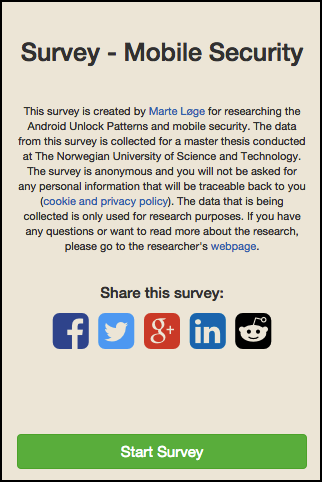
\includegraphics[scale=0.34]{pics/survey/start}
          \label{fig:startscreen}
        }
        \subfigure[ALP introduction]{
          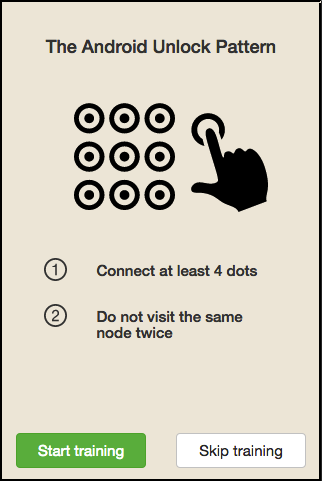
\includegraphics[scale=0.34]{pics/survey/rules}
          \label{fig:ALPintroduction}
        }
        \subfigure[Training mode]{
          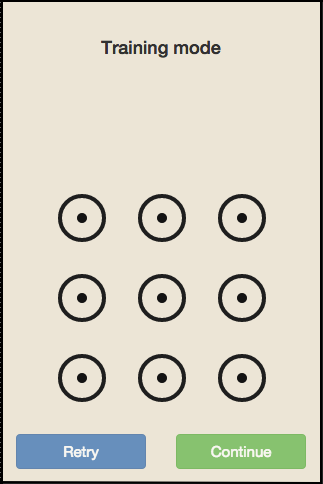
\includegraphics[scale=0.34]{pics/survey/training}
          \label{fig:trainingmode}
        }
        \caption{Survey screens}
        \label{fig:introductionviews}
      \end{figure}

    \subsection{Pattern Creation Process}
    After introducing the research and the Android Pattern Lock,  it is time to start collecting the three main selected patterns types; shopping account, smartphone, and banking account. The reason for dividing the pattern collection process into three separate patterns is to put the pattern creation into a context. The decision to add three patterns also works as a preventive measure for avoiding data being submitted by respondents just trying to finish the survey as fast as possible. 

    By introducing three separate pattern types instead of only one type, can introduce both positive and negative effects. When asking respondents to create a pattern for other types than its intended environment, some people might be confused. The choice of asking people to create a pattern for a banking account can for someone be an uncomfortable situation, might causing respondents to leave the survey. By asking the participants to create three patterns instead of one pattern takes more time and requires more attention and creativity from the participant. When asking respondents to create three patterns can introduce a situation where some respondents are creating the same pattern for all pattern types. 

    In the survey, respondents are asked to create a pattern for a shopping account, a smartphone, and a banking account. The three types are being carefully selected of how people would categorize different situations from a security point of view. As mentioned, the three pattern types are introduced to set the pattern creation process into context, avoiding dishonest attempts for answering the survey. 

    When collecting the patterns, it is desirable to copy the pattern creation process used by Android. The process consists of two steps: create a pattern of at least four connected dots, after that retype the same pattern for completing the process. Figure \ref{fig:androidpatterncreationprocess} shows the pattern creation process from a real Android smartphone. First, the user selects a pattern of at least four connected dots as illustrated in Figure \ref{fig:drawpattern}. Second, after creating a pattern, the user are asked to retype the same pattern as illustrated in Figure \ref{fig:confirmnewpattern}. If the redrawn pattern was correctly typed, the pattern creation process are finished. The pattern creation process used in the survey are visualized in Figure \ref{fig:patterncreationworkflow} and \ref{fig:createandretypepatterns}.

    \begin{figure}[H]
      \centering
      \subfigure[Draw pattern]{
        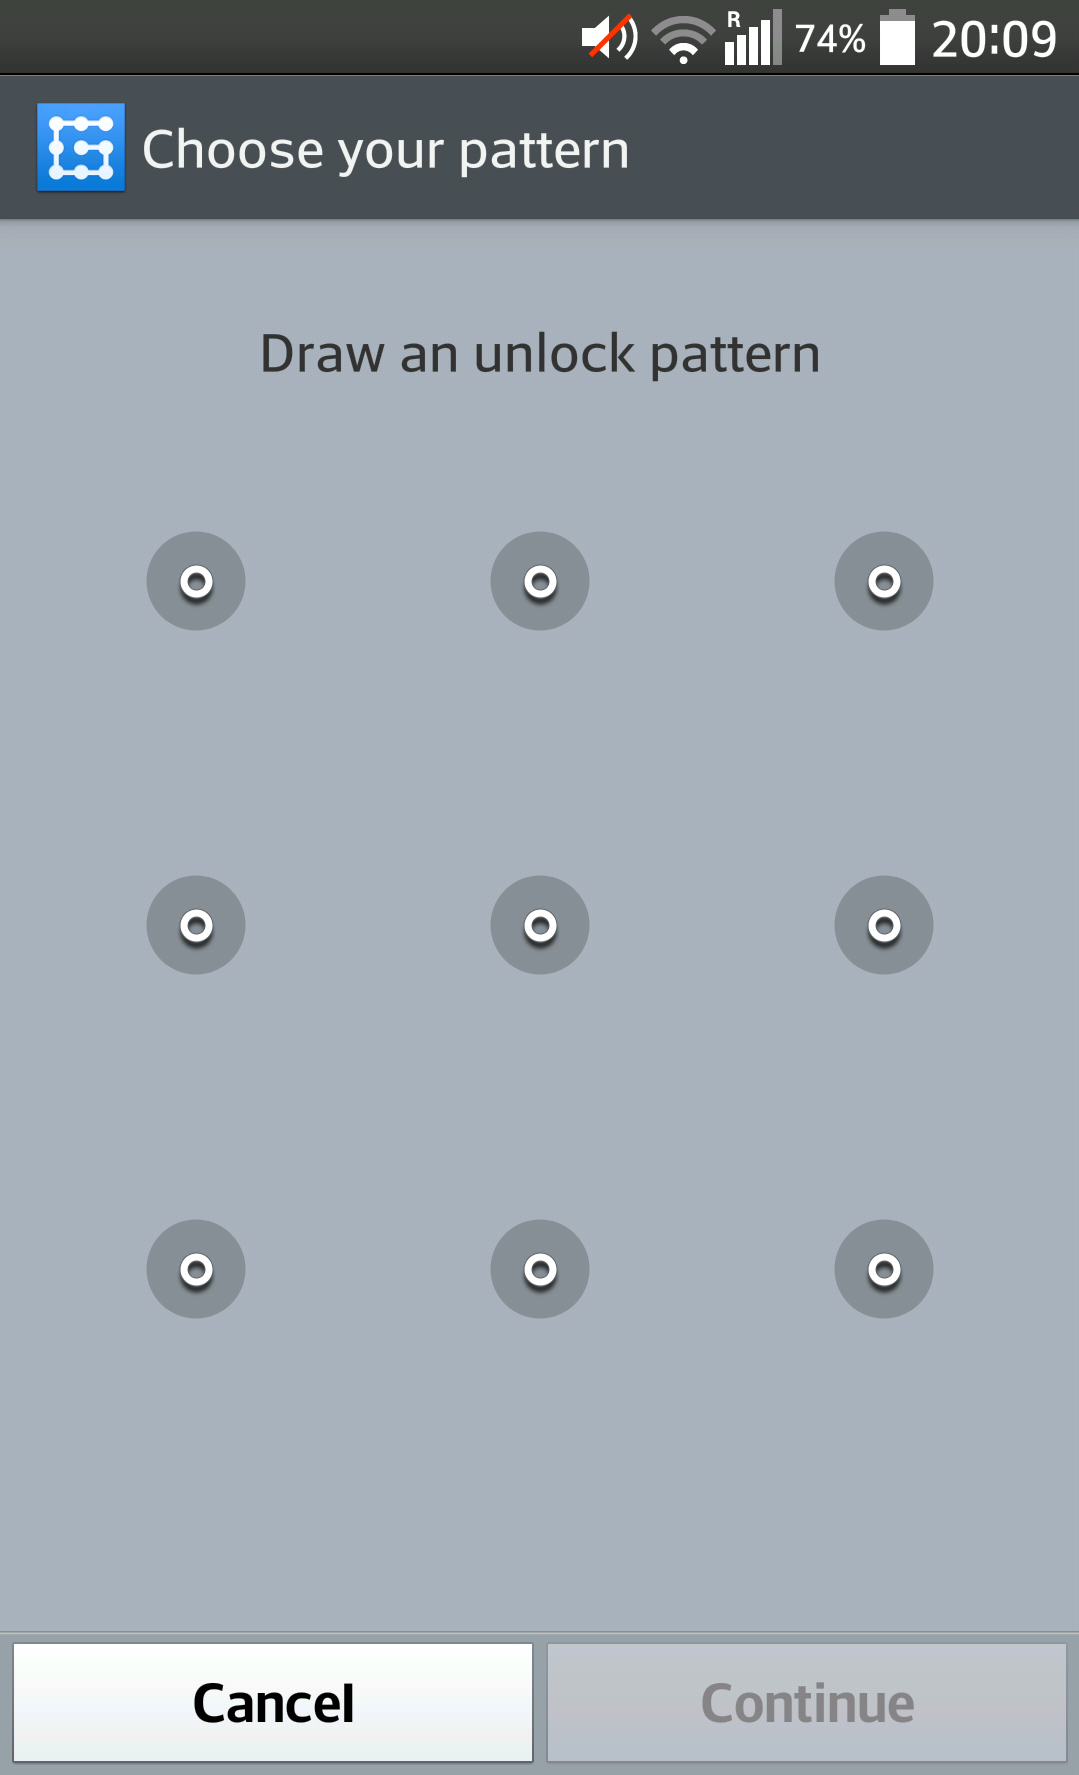
\includegraphics[scale=0.08]{pics/experiment/patternprocess3.png}
        \label{fig:drawpattern}
      }
      \subfigure[Pattern recorded]{
        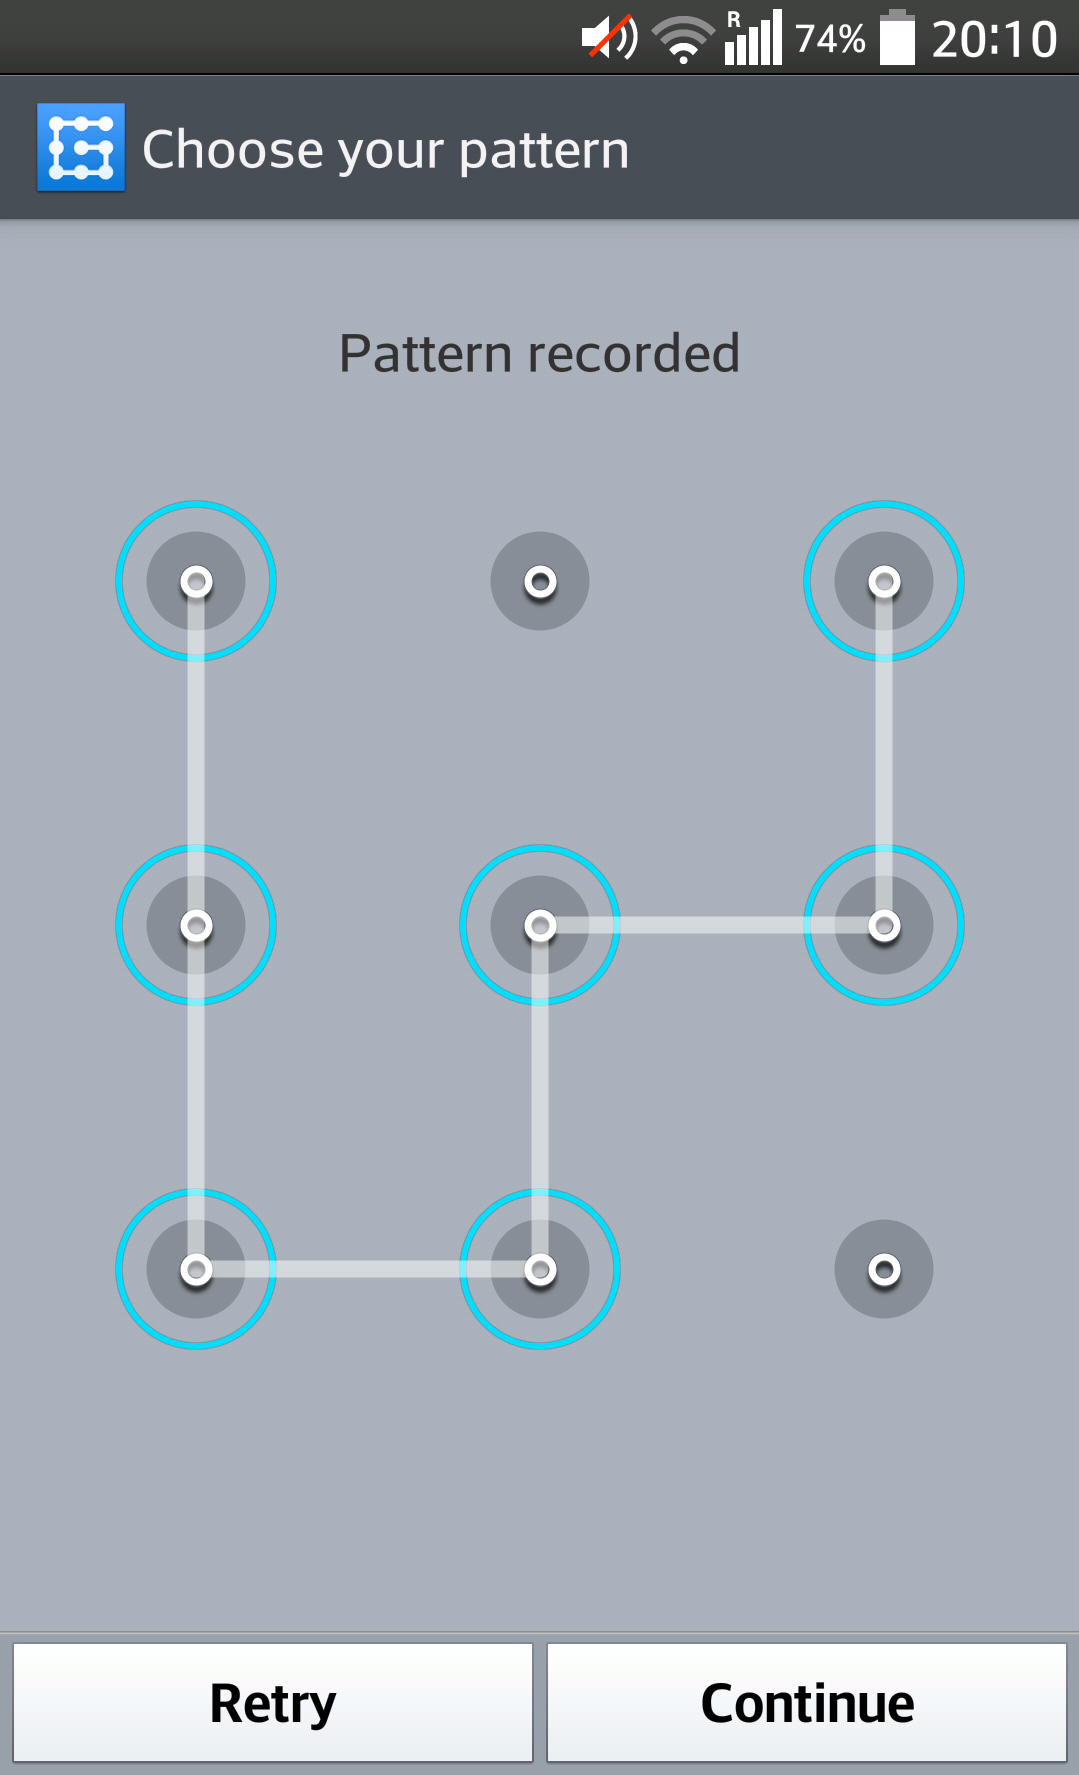
\includegraphics[scale=0.08]{pics/experiment/patternprocess4.png}
        \label{fig:patternrecorded}
      }\\
      \subfigure[Redraw pattern]{
        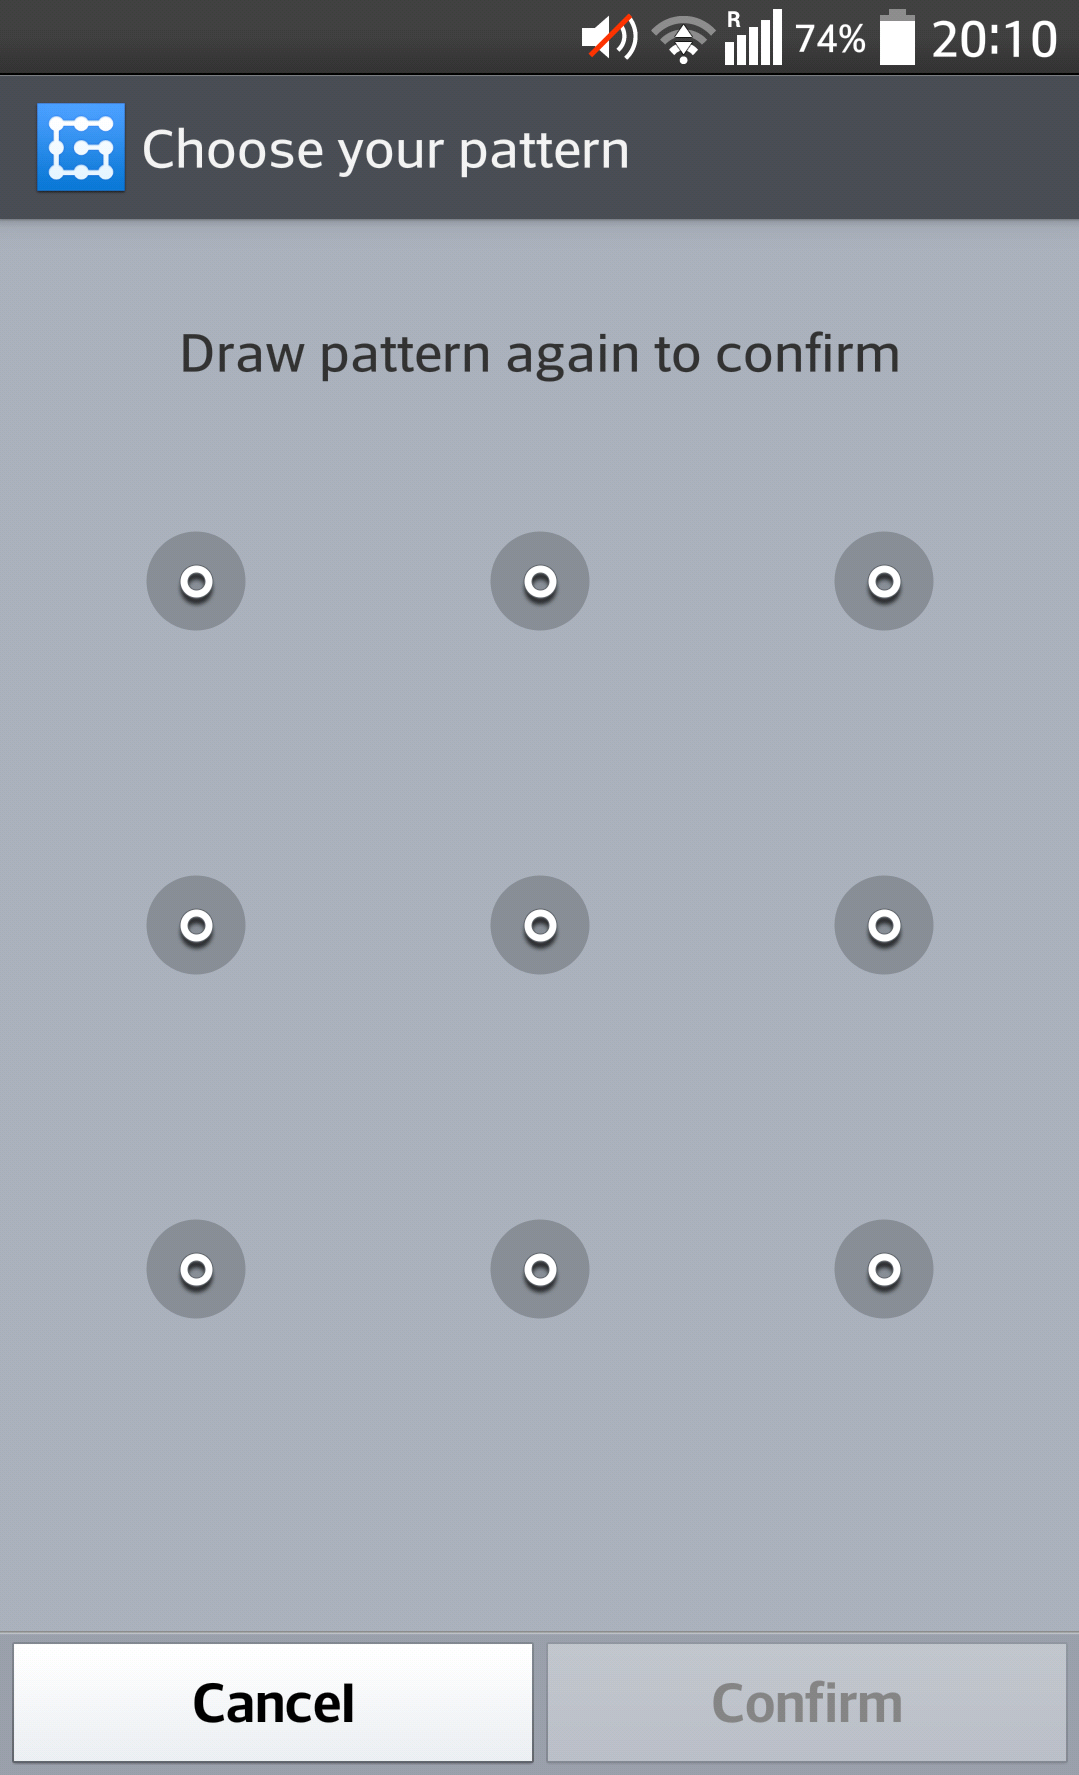
\includegraphics[scale=0.08]{pics/experiment/patternprocess5.png}
        \label{fig:redrawpattern}
      }
      \subfigure[Confirm new pattern]{
        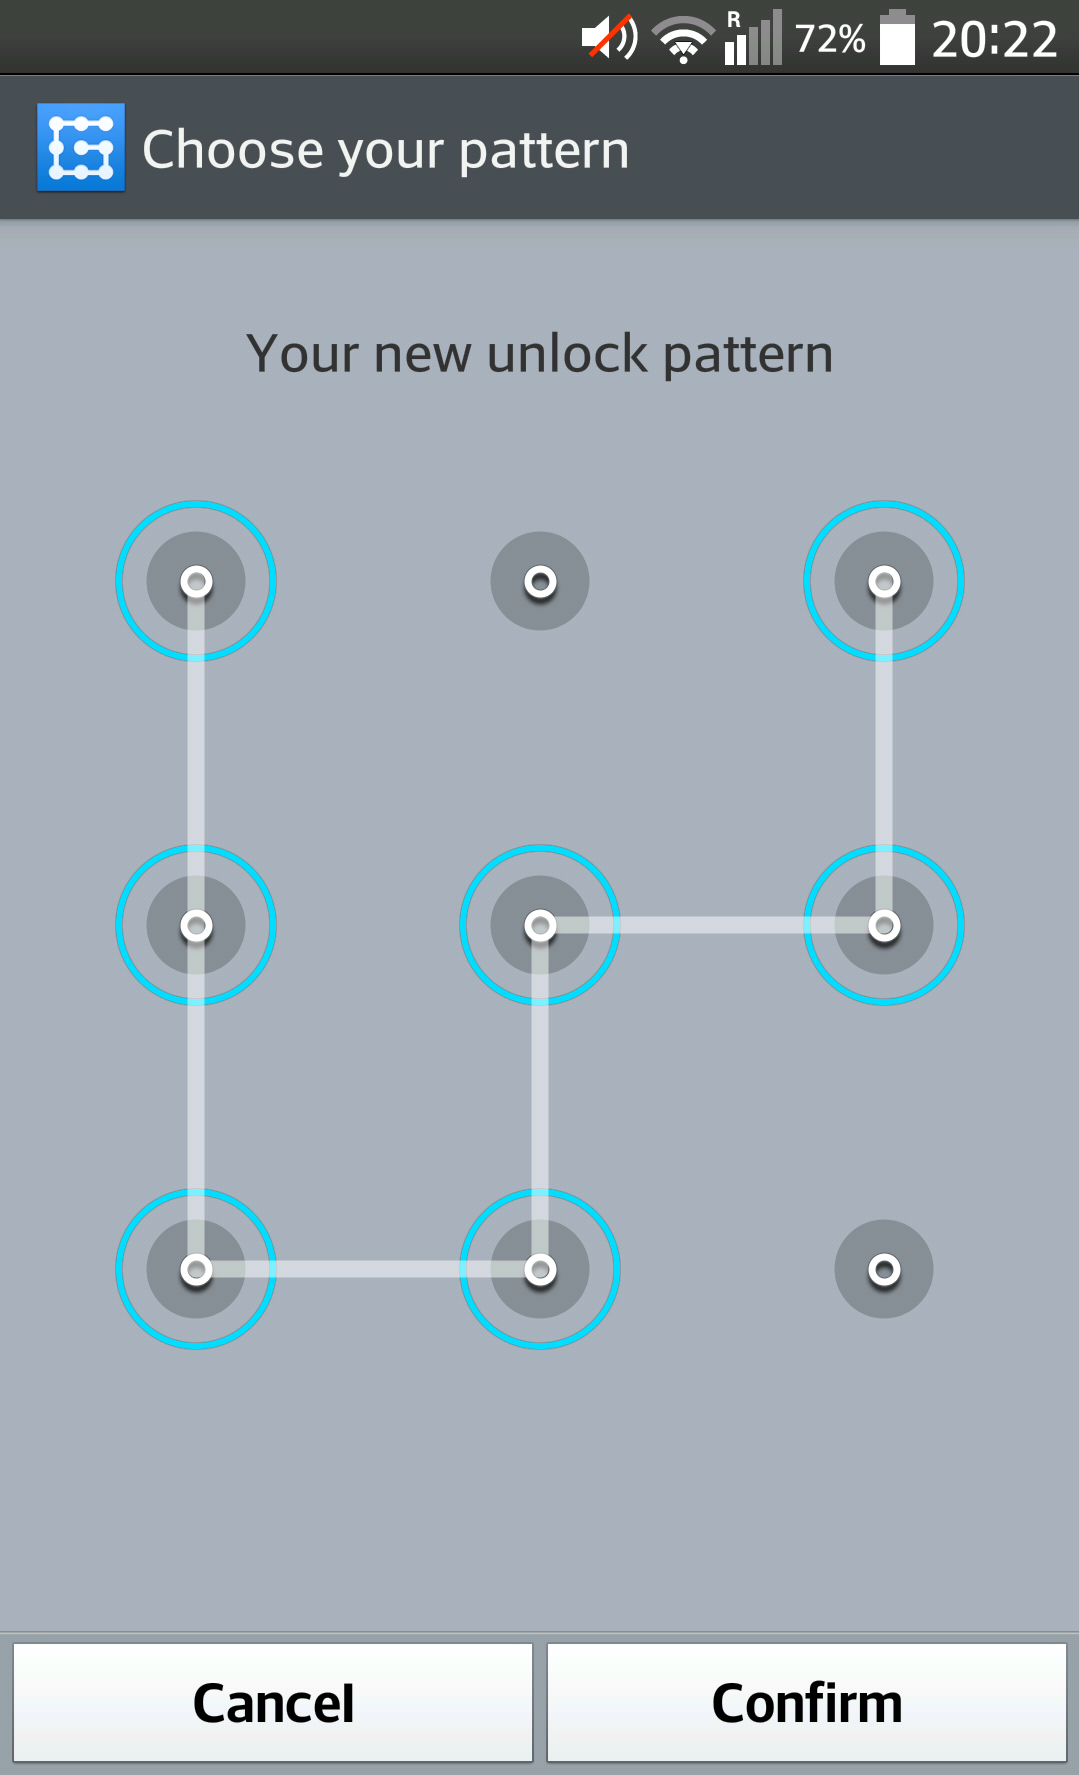
\includegraphics[scale=0.08]{pics/experiment/patternprocess1.png}
        \label{fig:confirmnewpattern}
      }
      \caption{The Android pattern creation process}
      \label{fig:androidpatterncreationprocess}
    \end{figure}

    \clearpage

    \begin{figure}[H]
      \centering
      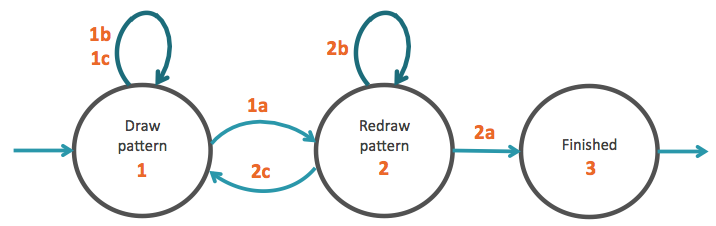
\includegraphics[width=\textwidth]{pics/experiment/patterncreationflow.png}
      \caption{Pattern creation workflow}
      \label{fig:patterncreationworkflow}
    \end{figure}

      \begin{enumerate}[leftmargin=0.3in]
        \item The first step is tp draw the pattern. The patter are drawn by connecting the nodes on the grid creating lines between the nodes (Figure \ref{fig:bankpattern}). The user will not be able to proceed before a valid pattern is drawn.
          \begin{enumerate}
            \item If the pattern is a valid pattern, the pattern turns green, and the message "pattern recorded" are shown. After, the user are able to press the {\it "Continue"} button to proceed to step 2 (Figure \ref{fig:validpatternrecorded}). 
            \item IIf the pattern not being valid pattern, the pattern turns red, and the message {\it "Connect at least 4 dots"} are shown (Figure \ref{fig:patternlengthtooshort}). The user can press the button {\it "Retry"}  for redrawing a new pattern.
            \item If a pattern drawn is a valid pattern, but the user want to create a different pattern, the user can always press the "Retry" button to reset the pattern already created. 
          \end{enumerate}
        \item When the respondent has created a valid pattern in step 1, they are proceeded to step 2 for redrawing the created pattern. The view is very similar to the view in step 1 beside the buttons and the text (Figure \ref{fig:retypepattern}).
          \begin{enumerate}
            \item If the user successfully redraws the pattern from step 1, the pattern turns green, and the message {\it "Correct!"} appears as in Figure \ref{fig:retypecorrect}. The user can complete the pattern creation process by clicking the green button {\it "Continue"} to proceed to step 3 and complete the pattern creation process.
            \item If the user unsuccessfully manages to redraw the pattern cerated in step 1, the pattern turns red, and the message "Not the same pattern" appears (Figure \ref{fig:retypewrong}). The user can try to remember the pattern and try to draw again. A situation like this can appear when the user do not remember the pattern or incorrectly draws the pattern.    
            \item If the user do not remember the pattern created at all, the {\it "Back"} button can be hit to go back to step 1 where the user are able to recreate a new pattern.  
          \end{enumerate}
        \item When the user successfully redraws the pattern in step 2, the pattern is successfully created.
      \end{enumerate}

    \begin{figure}[H]
      \centering
      \subfigure[Introduction to patterns]{
        \includegraphics[scale=0.3]{pics/survey/pattern-introduction}
        \label{fig:introductiontopatterns}
      }
      \subfigure[Shopping pattern]{
        \includegraphics[scale=0.3]{pics/survey/shopping}
        \label{fig:shoppingpattern}
      }
      \subfigure[Smartphone pattern]{
        \includegraphics[scale=0.3]{pics/survey/smartphone}
        \label{fig:smartphonepattern}
      }
      \subfigure[Bank pattern]{
        \includegraphics[scale=0.3]{pics/survey/bank}
        \label{fig:bankpattern}
      }
      \subfigure[Pattern length too short]{
        \includegraphics[scale=0.3]{pics/survey/not-valid-pattern-bank}
        \label{fig:patternlengthtooshort}
      }
      \subfigure[Valid pattern recorded]{
        \includegraphics[scale=0.3]{pics/survey/pattern-recorded-bank}
        \label{fig:validpatternrecorded}
      }
      \subfigure[Retype pattern]{
        \includegraphics[scale=0.3]{pics/survey/retype-bank}
        \label{fig:retypepattern}
      }
      \subfigure[Retype wrong]{
        \includegraphics[scale=0.3]{pics/survey/not-valid-retype-bank}@
        \label{fig:retypewrong}
      }
      \subfigure[Retype correct]{
        \includegraphics[scale=0.3]{pics/survey/retype-correct-bank}
        \label{fig:retypecorrect}
      }
      \caption{Survey - Create and retye patterns}
      \label{fig:createandretypepatterns}
    \end{figure}

  \clearpage 

  \subsection{Background Information}
    After going through the pattern creation process for the three pattern types, the respondent will now be asked several questions about their mobile and personal characteristics. Figure \ref{fig:surveyquestoins} shows screenshots from the survey application and the questions asked. The views in Figure \ref{fig:surveyquestoins} is the final design used used for collecting data. The changes made during the design and implementation are described in Section \ref{sec:usabilitytestingsurvey}. 

    There are some core functionality implemented in these questions that is important to notice. {\it First}, the traditional list of alternatives are replaced by icons. As discussed in Section \ref{sec:requirementstosurvey}, it is important to customize the interface for easy interaction on a mobile touchscreen. The images used are easy to interact with because of its size, and it requires less text because of the semantic meaning of the icons used. The icons used in the survey has been tested in a own usability test that are described later in Section \ref{sec:usabilityicontest}. {\it Second}, to keep the user motivated, a progress bar is added to the views. The questions are listed after their appearance in the survey. Not all the questions are visualized in figure \ref{fig:surveyquestoins}, but all will be described in in detail in this section. 

    The first questions to be asked is the handsize of the respondent, ranged from small to extra large as visualized in Figure \ref{fig:handsizeview}. The question is a subjective categorization, and there is no way of doing any countermeasures for avoiding wrong classification. There is often a difference in hand size of genders, so the question is asking the respondents to categorize the size of their hand according to their gender. By specifically asking for hand size based on gender will give a more precise answer. The male respondents claiming to have a small hand will probably have a bigger hand compared to female respondents claiming to have a the same size. 

    Figure \ref{fig:handednessview} and \ref{fig:screensizeview} are the handedness of the respondent and the size of the screen used, respectively. Whether a person should be straight forward, where your dominant are either left- or right-hand. Screen size has the same problem as asking for the hand size, because how a respondent categorizes the screen size depends on the subjective evaluation made by the respondent. A countermeasure for having the possibility to evaluate respondents categorization of the screen sizes is to store the size of the screen in pixels. The task of storing the pixel width and height of the screen are stored automatically when the respondent selects the screen size.

    Figure \ref{fig:fingerusedview} and \ref{fig:handusedview} is questions asking for the hand and finger used for creating the patterns. Typically, a respondent will either use their left or right hand for holding the smartphone while interacting with the screen by using either the forefinger or the thumb. The option of using another finger than forefinger and thumb are also applied. Instead of using words like thumb and forefinger, a circle is applied to a hand indicating the finger used. 

    Figure \ref{fig:readingandwritingview} are asking about the reading and writing direction preferred by the respondent. The three alternatives includes a small example to avoid any misinterpretation of the icons. Figure \ref{fig:genderview}, \ref{fig:ageview}, and \ref{fig:experiencewithITSecurity} are asking about the respondent's gender, age, and experience with IT and security. The alternatives for gender are visualized by using a male and female icon. The last question asks whether the respondent have any experience with IT and security. The screens missing from Figure \ref{fig:surveyquestoins} are the question asking for the screenlock the respondent use, country, and the last screen thanking the respondents for participating. 
    

  \clearpage

    \begin{figure}[H]
      \centering
      \subfigure[Handsize]{
        \includegraphics[scale=0.3]{pics/survey/handsize}
        \label{fig:handsizeview}
      }
      \subfigure[Handedness]{
        \includegraphics[scale=0.3]{pics/survey/handedness1}
        \label{fig:handednessview}
      }
      \subfigure[Screen size]{
        \includegraphics[scale=0.3]{pics/survey/screen}
        \label{fig:screensizeview}
      }
      \subfigure[Hand used when creating pattern]{
        \includegraphics[scale=0.3]{pics/survey/handedness2}
        \label{fig:handusedview}
      }
      \subfigure[Finger used]{
        \includegraphics[scale=0.3]{pics/survey/finger}
        \label{fig:fingerusedview}
      }
      \subfigure[Reading/writing direction]{
        \includegraphics[scale=0.3]{pics/survey/reading}
        \label{fig:readingandwritingview}
      }
      \subfigure[Gender]{
        \includegraphics[scale=0.3]{pics/survey/gender}
        \label{fig:genderview}
      }
      \subfigure[Age]{
        \includegraphics[scale=0.3]{pics/survey/age-2}
        \label{fig:ageview}
      }
      \subfigure[Experience]{
        \includegraphics[scale=0.3]{pics/survey/experience2}
        \label{fig:experiencewithITSecurity}
      }
      \caption{Survey - Questions}
      \label{fig:surveyquestoins}
    \end{figure}

    \clearpage

    There is one special question in the survey that is not being mentioned until now; the mobile operating system used. This question is one of the hard questions to ask because it is no intuitive way for asking about the operating system of a mobile without using any technical terms. 

    Instead of listing all the possible mobile operating systems for mobile devices, the mobile operating system of the mobile is detected and visualized. In other words, the survey checks for the mobile OS and present what is being detected. With this information, a generic question like {\it "Is this your mobile operating system?"}, hence avoiding a long list asking {\it "Which one is your mobile OS?"}. The alternatives presented, \texttt{Yes}, \texttt{No}, and \texttt{Don't know}, are designed in way that the answer provided by the respondent are valuable whatever they select. For each mobile OS, each corresponding alternative are stored as \texttt{mobileOS\_yes}, \texttt{mobileOS\_no}, and \texttt{mobileOS\_unknown}.

    When the OS have been detected, one of the screens in Figure \ref{fig:mobileOSquestion} will show. It is implemented support for four different mobile operating systems that are covering the majority of the operating systems on smartphones: iOS, Android, Windows, and BlackBerry. Each OS will have the three alternatives yes, no, and question mark. 

    One pitfall is the formulation of the question. I should avoid any formulations stating that I detects their information. A question like {\it "It is detected that you have an Android phone. Is this correct?"} can be daunting, hence causing the respondents the feeling of being monitored. The feeling of someone knowing anything about you can be scary for anyone not knowing the technical details. The mobile operating system are easily detected on the client side with one line of code with {\it JavaScript}.

    \begin{figure}[H]
      \centering
      \subfigure[iOS]{
        \includegraphics[scale=0.34]{pics/survey/ios}
      }
      \subfigure[Android]{
        \includegraphics[scale=0.34]{pics/survey/android}
      }
      \subfigure[Windows]{
        \includegraphics[scale=0.34]{pics/survey/windows}
      }
      \caption{Survey - Mobile OS}
      \label{fig:mobileOSquestion}
    \end{figure}
    \clearpage

    Figure \ref{fig:thefadingeffect} shows an example of what happens when the respondent clicks on an icon. When an icon is being press, the icons are highlighted by turning green like in Figure \ref{fig:selecticon}. When an icon is being clicked on, a slow fading effect starts for indicating the state changes to the next question. The fading effect are visualized in Figure \ref{fig:iconfadingout} and \ref{fig:iconfadedout}. When the question is faded out, the next question appears. The fading effect implemented is a cause of the described navigation requirements stated in Section \ref{sec:requirementstosurvey}. By using the automatic navigation while clicking on an image, the highlighting and the fading effect supports the respondent keeping track of the state. If a view is not utilizing icons, the fading effect is still used for indicating a change of state.

    \begin{figure}[H]
      \centering
      \subfigure[Select icon]{
        \includegraphics[scale=0.34]{pics/survey/icon-selected-1}
        \label{fig:selecticon}
      }
      \subfigure[Icon fading out]{
        \includegraphics[scale=0.34]{pics/survey/icon-selected-3}
        \label{fig:iconfadingout}
      }
      \subfigure[Icon faded out]{
        \includegraphics[scale=0.34]{pics/survey/icon-selected-4}
        \label{fig:iconfadedout}
      }
      \caption{Survey - Icon selecting effect}
      \label{fig:thefadingeffect}
    \end{figure}

	% !TEX root = ../main.tex
\section{Usability Testing of the Survey}\label{sec:usabilitytestingsurvey}

  The usability of the survey was tested for different purposes. {\it First}, when sending out the survey, there is no much room for changing the layout and content of the survey. When changing the survey during the data collection process, it could introduce bias in the data because the participant could interpret the changed content in different ways. {\it Second}, the survey is in a non-controlled environment, meaning that I have no control of who the participants are and where they are from. It is important to make the layout and the questions as universal an understandable as possible. The questions, the flow, and the graphical elements should be understandable across different countries and cultures. 

  The usability testing is divided in two main parts: usability testing in a controlled environment and usability testing in a uncontrolled environment. Beside the specific usability tests performed, it was also conducted a smaller test only focusing on the icons used in the survey.

    \subsection{Testing the wireframes}


    \subsection{Testing the icons used in the survey}\label{sec:usabilityicontest}
      Legge til resultatene som ble gjort her.

  	\subsection{Testing the application in a controlled environment}
    A usability test in an uncontrolled environment...
    Previous test results....

    The test was conducted with 10 students, 5 boys and 5 girls, from the Norwegian University of Science and Technology. The participants had different background, but the majority had a background in Computer Science.

    To ensure the test was conducted in an environment that is close to how the survey works, they brought their own smartphone and they were not told much about the research. They only got a short introduction to the test that would not impact the results from the test. The participants were told how the test would be performed:

      \begin{enumerate}
        \item The participant were asked to speak loud during the test and tell what they were thinking and reason about their choices.
        \item The participants were told that the test was not testing their ability to finish the test.
        \item The participants were explained that they could quit the test if they felt uncomfortable
      \end{enumerate}

    After giving a introduction to the test, the participant got the URL to the survey and they were asked to start whenever they felt ready. In the list below there is listed comments from the participants that was stated during the test.
        
    {\it "How do I get back if I press a wrong answer?"}\\ 
    One of the persons asked how he could get back to previous question if he selected the wrong answer. He expected a button that could take him back to the previous question.
    
    {\it "Too much icons in the screen showing different screenlocks"}\\ 
    The person did find it confusing with all the icons showing the different screenlocks. The  also found it hard to select the correct screenlock that he used on his smartphone. He commented that this should be solved in a other way that would eliminate the ambiguity and confusing visualization with too many icons. One suggestion was to add a description to each of the icons in a list.
      
    {\it "I need to choose a pattern that is hard to guess for the banking account!"}\\ 
    Most of the participants used more time creating a pattern for a banking account than for the other patterns. Some of them also commented that they did spend more time creating this than the other patterns. It was also noticeable that the participants used more time thinking about this pattern.
    
    {\it "Do I choose the size of my hand based on my gender or is it general?"}\\ 
    Four of the participants was unsure how to categorize the size of their hand. Some of the participants also commented that they selected the size based on their gender or unisex.
      
    {\it "Tody my smartphone would probably be categorized as a medium smartphone"}\\The question is in general subjective, but there is no easy way to ask about the screen size. This question might depend on the persons technical experiences with smartphones. Today, most of the smartphones would be categorized as medium, while older smartphones might would fall into the small category.
      
    {\it "I expected to type the pattern more than once"}\\ 
    One of the participants commented that she expected to be asked to type the pattern more than once. She did not specify if she expected to be prompted with a retype right after creating the pattern or in the end of the survey.
      
    {\it "I do read from left to right, but I do also read lines from top to bottom."}\\ 
    Three of the participants either was unsure what the question asked about or did not understand the icons used. 
      
    {\it "I can't see the question becuase the pattern is too big for my screen"}\\
    One of the participant had a small older iPhone that where the survey rendered poorly because the pattern was too big. 
      
    {\it "The last question about my experience with IT and security took a while to understand."}\\ 
    The question was long and complex. Many of the participants used a long time interpreting the question and some of them asked me during the test if they had understood the question correctly.

    \subsection{Testing the application in a uncontrolled environment}
    Observation of incoming data is not a typical usability test, but is rather a quality check to see whether the collected data is reasonable. When sending out the survey on the internet without being present, it is important to quality check the data to see if it looks like some questions or the graphical elements are ambiguous or hard to understand.The survey was first deployed and distributed to a small group of selected people from Norway (ISO country code 'NO').

    After a day, I looked through the data. One of the observations was that one person had selected a quite rare and small country in Africa with the ISO country code starting with 'N'. It is reasonable that this was a typing error or something wrong with the component used in the question. The component used in the question was a third party dropdown list with a flag icon for each country. I found out that the country component took a long time loading and it appeared that it lagged. A possibility is that the person accidentally had selected the wrong country. The component changed and optimized to avoid this situation by changing the component and removing the icons due to reduce loading time.

    The majority of the people would be from Scandinavia and would have the reading direction form left to right. There was observed that 2 persons out of 25 had other reading and writing directing than left to right. Based on statistics, there should only be persons with reading and writing direction from left to right. One assumption is that the two persons selecting an other reading and directing had interpreted the question wrong. This question should be changed to avoid such situation. 

    Besides looking at the data, I received feedback by email from the selected group of persons.

    {\renewcommand\labelitemi{}
    \begin{itemize}
      \item {\it "The dropdown lagged and I accidently selected the wrong country."}
      \item {\it "I use a 8 digit PIN. Should I select PIN code, password or other?"}
    \end{itemize}}


  	\subsection{Changes to the Survey}

  	Before going live with the survey there was conducted two types of tests providing useful insight of how the users experienced the application. The tests is very important due to the quality of the data collected from the survey. Any ambiguities or errors would could cause bias in the data. After the test I would go through all the feedback and the observed data to make any changes needed in the survey.

    \subsubsection*{1) Country dropdown}
    In both tests there was many participants that unintentionally selected the wrong country because the dropdown component lagged. The component used had a flag attached to the country name that used a lot resources to load, and therefore some user experienced that the component was slow. The component was changed and the flag icons were removed. The changes can be seen in Figure \ref{fig:change-country}.

    \subsubsection*{2) Experience question}
    The question was rather complicated and hard to read. The question was changed from "Do you work with or study/studied IT and/or security full time?" to "Do you have a background in IT/Security?".
      
    \subsubsection*{3) Reading and writing direction}
    The first version of the survey just listed three different icons of arrows indicating the reading and writing direction, but it seemed that people misunderstood the icons in some way. This view was changed by adding a description next to the arrow in order to remove any misinterpretations of the directions. The changes are shown in Figure \ref{fig:change-readwrite}.

    \subsubsection*{4) Adding time used on the creation of patterns}
    It was observed that some of the participants in the usability test in the controlled environment was spending more time creating the pattern for banking account. During the test it was not easy to track the time used on different tasks, but it is possible to track the time used on each pattern in the application to see the diversity between the three types. The observation from the test was that some of the participants took their eyes of the screen thinking harder about the pattern they wanted to create for the bank. In this particular test I was present and could observe such situations, but I will not be able to do this in the application and therefore I added the time used. Such time frame can also be used in the analysis. An example of use could be to pick out dishonest attempts that could cause bias in the data. 
      
    \subsubsection*{5) Selection of screenlock}
    The first version of the view had a list of all the screenlocks that are normally used on a smartphone. The feedback from the tests was that is was confusing to select the correct screenlock for several reasons. {\it First}, some of the participants did not understand all the icons used. {\it Second}, it was observed that some of the user did not interpreted all the alternatives and selected the first fit, but it was sometimes wrong when I stopped the user and asked what they actually used. {\it Third}, it appears that some had a screenlock that could fit into several of the icons, making it hard to pick the correct one. The new version of the view replaced all the icons to a dropdown with alternatives. When the user selects a screenlock, a image or description appears below the dropdown so they could get a extra layer of confirmation that they had selected the correct screenlock. The alternative "PIN" was also changes to "PIN (4-digits)" to be specific and eliminate any ambiguity for those who use more than four digits. The reason for specifically choose four digits is because most users are familiar with this at their bank and smartphones. The changes in this view can be seen in Figure \ref{fig:change-screenlock}.
    
    \subsubsection*{6) Scaling pattern selector for smaller devices}
    The 3 times 3 pattern square was set to a specific size based on the width of the screen, but it seemed that some mobile screen lost some of the height from browser navigation bars. As a consequence, the pattern was laying over the question, making it hard to see which pattern they where creating. There was added a mathematical formula to ensure that the pattern square was scaling properly on any screensize. 
    
    \subsubsection*{7) Changing handsize question}
    Based on feedback in the test in the controlled environment, the participants did not know what to compare their handsize to. They often reasoned different sizes compared to their gender and unisex. It was therefore desirable to explicitly state in the question that the user was selecting their size of their hand based on their gender. The question still remains subjective, but by explicitly stating gender as a standard it will remove some bias. 
    
    \subsubsection*{8) Adding pattern retype}
    During the tests I god feedback that many of the participants expected to be asked to retype their selected patterns right after creating it or in the end of the survey. It is not desirable to ask users to retype their patterns in the end of the survey because users then would feel uncomfortable if they did not remember it. It did not want the users to leave the survey with a bad experience. By stating that the users should remember the patterns in the end of the survey could end up with many user leave the survey because they would feel uncomfortable. Some would might also leave the survey because it would require them to actually do more work than they are willing to do for a survey. I decided to ask the user to retype the pattern right after creating because this is how the process works on Android smartphones. On Android devices, the users types a pattern and are thereafter asked to retype the pattern again to create the pattern for their smartphone. \todo{Visualize process in survey and on Android. The pattern cre. proc.}
    
    \subsubsection*{9) Collecting screen pixels of screen used}
    By observing the participants in the first test, I recorded my opinion of their screen size as well as their own choices. About 70\% of their choices matched my own opinion of the screen size. Since this question is a subjective meaning of the person answering, I added an extra layer of information by saving the pixels width and hight of the mobile device. One problem with pixels size of a mobile screen is that they do not match the physical size of the screen. The pixels could still provide information to actually categorize the correct size by comparing the OS and pixels.

    \begin{figure}[H]
      \centering
      \subfigure[Old view]{
        \includegraphics[scale=0.34]{pics/survey/country-old}
      }
      \subfigure[Final view after changes]{
        \includegraphics[scale=0.34]{pics/survey/country2}
      }
      \caption{Changes in country selection view}
      \label{fig:change-country}
    \end{figure}

    \begin{figure}[H]
      \centering
      \subfigure[Old view]{
        \includegraphics[scale=0.34]{pics/survey/reading-old}
      }
      \subfigure[Final view after changes]{
        \includegraphics[scale=0.34]{pics/survey/reading}
      }
      \caption{Changes in reading/writing direction view}
      \label{fig:change-readwrite}
    \end{figure}

    \begin{figure}[H]
      \centering
      \subfigure[Old view]{
        \includegraphics[scale=0.34]{pics/survey/screenlock-old}
      }
      \subfigure[Final view after changes]{
        \includegraphics[scale=0.34]{pics/survey/screenlock2}
      }
      \caption{Changes in screenlock selection view}
      \label{fig:change-screenlock}
    \end{figure}

% -  --> Changed third party component
% -  --> Changes question
% -  --> Added description
% - 
% -  --> Changed to dropdown list
% -  --> 6 different orders.
% - 
% - Question about handsize --> Based on gender
% - Pattern retype --> same process as android
% - Screensize

	% !TEX root = ../main.tex
\chapter{Results}\label{chap:results}

	Nevne noe om hvor det står mer detaljer om pattern strength slik at man slipper å ta den samme korte oppsummeringen i hvert delkap???

	%TIME
	When creating a pattern in the survey, both time used to create a pattern and the actual pattern created was recorded. The time used to create the pattern was recorded from the start when the grid appeared until the user submitted the pattern.

	%LENGTH
	The pattern length are defined as the number of dots used to form a pattern. Each dot have a own sequence number and can only appear once. The minimum length of a pattern is 4 and the maximum length is 9. The number of unique patterns of all possible pattern lengths are described in table \ref{tab:combinations}. The pattern length are visualized in two different ways; the average pattern length and the distribution of pattern length.

	....pattern length distribution indicating what pattern length that are more often selected by the population.

	%VISUAL COMPLEXITY 
	Pattern complexity, e.g. pattern strength, is calculated from a mathematical formula that take into account the different aspects of visual complexity of patterns. The formula and parameters used are described in detail in Section \ref{sec:alp}. In short, the formula uses the size (number of nodes), physical size (length) of the pattern, number of intersections and number of overlaps. The minimum strength is 6.340 and the maximum strength is 46.807.

	%Rensing av data
	-- MAX tid feks 


	\todo[inline, color=green!60]{Referere tilbake til literaturstudie i resultatene!}
	\todo[inline, color=green!60]{Referere til kildene for pattern strength (paper)}
	
	% !TEX root = ../main.tex
\section{The Population} \label{sec:basicstatistics}
  
  This chapter will be a summary of the basic statistics aggregated from the collected data. Basic statistics is defined as statistics where data are only aggregated and presented as is where no other algorithm or mathematical formulas have been used.

  Background information is the data representing some fundamental aspects on the collected data. This section will go though the data represented in Table \ref{tab:respondentsBasics}, Table \ref{tab:screenlockHabits}, Table \ref{tab:country}, and Figure \ref{fig:ageDistribution} summarizing the basic statistics of the collected data. 

  Table \ref{tab:respondentsBasics} is a overview of the respondents summarizing the frequency of respondents, gender, handedness, their experience with IT and security, and reading/writing orientation. In total 802 respondents completed the whole survey by answering all questions. 11 participants started creating pattern and answering, but stopped before completion. 204 people started creating patterns and stopped before creating all three types of patterns. 81 persons entered the survey and left without leaving any information. 

    %Table: Summary of the background information
    \begin{table}[H]
      \parbox{.45\linewidth}{
        \centering
        \begin{tabular}{ l | l l }
          \hline
          \multicolumn{3}{l}{\bf Respondents} \\ \hline
          Completed survey & 802 \\
          Stoped during survey & 11 \\
          Started creating patterns & 204 \\
          Opened survey and left & 81 \\ \hline
            
          \multicolumn{3}{l}{\bf Gender} \\ \hline
          Male & 529 & 66\% \\
          Female & 278 & 34\% \\ \hline

          \multicolumn{3}{l}{\bf Handedness} \\ \hline
          Left & 97 & 12\% \\
          Right & 690 & 88\% \\ \hline

          \multicolumn{3}{l}{\bf Experience with IT/Security} \\ \hline
          Yes & 470 & 59\% \\
          No & 332 & 41\% \\ \hline

          \multicolumn{2}{l}{\bf Reading/Writing direction} \\ \hline
          Top-to-bottom & 7 & 1\% \\
          Right-to-Left & 8 & 1\% \\
          Left-to-right & 792 & 98\% \\ \hline
        \end{tabular}
        \caption{Summary of the respondents}
        \label{tab:respondentsBasics}
      }
      \hfill
      \parbox{.45\linewidth}{
        \centering
        \begin{tabular}{ l | l l }
          \hline
          \multicolumn{3}{l}{\bf Mobile Operating System} \\ \hline
          Android & 464 & 58.0\% \\
          iOS & 321 & 40.0\% \\
          Windows & 16 & 1.9\% \\
          Blackberry & 1 & 0.1\% \\ \hline
 
          \multicolumn{3}{l}{\bf Used Android Unlock Pattern} \\ \hline
          Yes & 526 & 65\% \\ 
          No & 278 & 35\% \\ \hline

          \multicolumn{3}{l}{\bf Use screenlock} \\ \hline
          Yes & 655 & 82\% \\
          No & 149 & 18\% \\ \hline

          \multicolumn{3}{l}{\bf Screenlock in use} \\ \hline
          Android Pattern Lock & 202 & 31\% \\
          4-digit PIN & 237 & 36\% \\
          Fingerprint & 116 & 18\% \\
          Password & 44 & 7\% \\
          slide-to-unlock & 28 & 4\% \\
          Other & 28 & 4\% \\ \hline
        \end{tabular}
        \caption{Screen lock habits}
        \label{tab:screenlockHabits}
      }
    \end{table}

    Out of the persons entering their gender, 66\% of the participants were male and 34\% were female. Looking at handedness of the participants, 88\% were right-handed and 12\% were left-handed. The percentage of left-handedness in the population is hard to estimate, but it is stated that about 10\% of the population are left-handed \cite{lefthandedness} that seems reasonable with the percentage of left-handed participants from the survey. The reason why the percentage is somehow higher is because the survey was sent to a group of left-handed people that can be the reason for getting 12\% instead of 10\% left-handed participants.
    
    To be able to distinguish between people with experience with IT and Security it was asked about the participants experience in the survey. The network of myself and both supervisors are heavily overrepresented by people in the field of IT and Security. People with this background will might cope with the security related questions in a different way than people without the experience with IT and security. The data shows that the majority, 59\%of the respondents, had a background within IT and Security while 41\% did not. 

    It is hard to reach people outside your own network, especially to reach groups of people with a other cultures. In the dataset it was only 2\% that had an another reading and writing direction, top-to-bottom and right-to-left, than the other participants that read and writhe from left-to-right. Countries operating with a reading and writing direction are often Arabic countries or countries located in Asia. The problem is that many of these countries have during the past years been influenced from western countries. The first problem is to reach people with other reading and writing orientation than myself because all people i know read and write from left to right. I can therefore not make any further statistical analysis comparing people with different reading and writing orientation because the number of participants with that characteristics are too low to get any significant results.

    Table \ref{tab:screenlockHabits} summarized the respondents screenlock habits looking specifically at their experience with the Android Unlock Pattern, their use of screenlock mechanisms, and which screenlock they are currently using. This will provide as a overview of how people cope with security on their smartphones. Because different mobile operating systems provides different security mechanisms, the mobile operating system are also added to the table. It is not a surprise that the majority have answered the survey using either a mobile with a Android or iOs operating system that are the most popular in the the market at this point of time. 

    A total of 65\% of the participants have used the Android Pattern Lock before. The 35\% not familiar with the Android Pattern Lock will probably have their first time using the Android Pattern Lock. There will might be many experienced people with the Android Pattern Lock but it is not given that they are still using it. There are in total 82\% of the participants not using any screenlock and 18\% not using any screenlock. Among the listed screenlocks, the majority are using 4-digit PIN, Android Pattern Lock and fingerprint. The fingerprint are only available at iPhone, while Android Pattern Lock are not allowed on iPhones.

    \clearpage  

    Figure \ref{fig:ageDistribution} shows a distribution of the respondents age. The respondents are divided into 8 intervals: under 20, 20-24, 25-29, 31-34, 35-39, 40-49, 50-59, and over 60. The three last intervals have a lower frequency of participants and have therefore not being divided further into smaller intervals. The distribution have a peak at the interval 20-24. Reasons for the skewed distribution can might be a cause of the network that received the survey. The majority of my own network are students in their twenties and can therefor introduce this skewed distribution. There are still other age intervals represented in the dataset. The higher the age, the lower the frequency of respondents. This can be the same cause as for the peak, but can also be slightly lower respondents over 40 because they do not own a smartphone, nor participate in the networks where the survey were published.

    %Figure: Age distribution
    \begin{figure}[H]
      \centering
      \includegraphics[scale=0.8]{pics/analysis/AgeDist.png}
      \caption{Age distribution}
      \label{fig:ageDistribution}
    \end{figure}

    The survey asked the participants about their country of origin. The data collection ended up with a 39 countries represented in the data set where the majority of the countries was Norway, United States of America as seen in Table \ref{tab:country}.

    This data can not be used to make any analysis on any specific county. During the data collection it was a goal to avoid a homogeneous dataset. The majority of the participants is still from Norway, but is was important to get other countries represented as well to obtain as a more heterogeneous data set. 

		%Table: Country of origin (39 countires)

   {\renewcommand{\arraystretch}{2}%

		\begin{table}[H]
	    \centering
	    \begin{tabular}{ l c | c }
	      \hline
	      \multicolumn{2}{c|}{\bf Country} & {\bf \# Respondents} \\ \hline
	      \raisebox{-.4\height}{\includegraphics[scale=0.4]{pics/flags/Norway.png}} & Norway & 517 \\ \hline
	      \raisebox{-.4\height}{\includegraphics[scale=0.4]{pics/flags/USA.png}} & United States of America & 115 \\ \hline
	      \raisebox{-.4\height}{\includegraphics[scale=0.4]{pics/flags/Germany.png}} & Germany & 33 \\ \hline
	      \raisebox{-.4\height}{\includegraphics[scale=0.4]{pics/flags/CzechRepublic.png}} & Czech Republic & 31 \\ \hline
	      \raisebox{-.4\height}{\includegraphics[scale=0.4]{pics/flags/UnitedKingdom.png}} & United Kingdom & 22 \\ \hline
	      \raisebox{-.4\height}{\includegraphics[scale=0.4]{pics/flags/Russia.png}} & Russia & 13 \\ \hline
	      \raisebox{-.4\height}{\includegraphics[scale=0.4]{pics/flags/Denmark.png}} & Denmark & 7 \\ \hline
	      \raisebox{-.4\height}{\includegraphics[scale=0.4]{pics/flags/Sweden.png}} & Sweden & 6 \\ \hline
	      \raisebox{-.4\height}{\includegraphics[scale=0.4]{pics/flags/Switzerland.png}} & Switzerland & 6 \\ \hline
	      \raisebox{-.4\height}{\includegraphics[scale=0.4]{pics/flags/Australia.png}} & Australia & 5 \\ \hline
	      \raisebox{-.4\height}{\includegraphics[scale=0.4]{pics/flags/Netherlands.png}} & Netherlands & 4 \\ \hline
	      \raisebox{-.4\height}{\includegraphics[scale=0.4]{pics/flags/Chile.png}} & Chile & 4 \\ \hline
	      \raisebox{-.4\height}{\includegraphics[scale=0.4]{pics/flags/Finland.png}} & Finland & 3 \\ \hline
	      \raisebox{-.4\height}{\includegraphics[scale=0.4]{pics/flags/Austria.png}} & Austria & 3 \\ \hline
	      \raisebox{-.4\height}{\includegraphics[scale=0.4]{pics/flags/Ukraine.png}} & Ukraine & 3 \\ \hline
	      \raisebox{-.4\height}{\includegraphics[scale=0.4]{pics/flags/China.png}} & China & 3 \\ \hline
	      \multicolumn{2}{p{8cm}|}{Afghanistan, Mexico, North Korea, Pakistan, Vietnam, Luxembourg, Ireland, Tunisia} & 2 \\ \hline
	      \multicolumn{2}{p{8cm} |}{Italy, Greece, Belgium, Indonesia, Malaysia, Bahrain, Botswana, Argentina, Singapore, japan, Canada, South Korea, Hungary, Turkey, Brazil} & 1 \\ \hline
	    \end{tabular}
	    \caption{Respondents country of origin}
	    \label{tab:country}
	  \end{table}

  {\renewcommand{\arraystretch}{1}%
    



	% !TEX root = ../main.tex
\section{Findings for the Entire Population}
  
  This section will go through the results from the survey based on the entire population. 
  \todo[inline, color=blue!60]{The data used in this section are preprocessed. The procedures can be found in section.}

	\subsection{Pattern Creation Time}
    Figure \ref{fig:avgpatterncreationtimepopulation} gives the pattern creation time in seconds for the three pattern types. By looking at the average creation time for patterns, patterns created for bank accounts have the highest creation time of 9.42 seconds while patterns created for smartphones have an average creation time of 8.24 seconds. 

    Figure \ref{fig:patterncreationtimeexperience} shows the average pattern creation time in seconds for respondents experienced with the Android Unlock Pattern. The graph reveals that both patterns created for shopping account and banking account are not affected by the participants experience with the Android Unlock pattern.

    Patterns created for smartphones have a lower response time for patterns created by respondents experienced with the Android Lock Pattern. Patterns created for smartphones by experienced respondents had an have an average creation time of 7.20 seconds while the patterns created for smartphones by unexperiences respondents had an average creation time of 8.40 seconds. The difference in average creation time results in a difference of 1.2 seconds. 

		\begin{figure}[H]
      \subfigure[Average pattern creation time (seconds)]{
        \includegraphics[scale=0.48]{pics/analysis/avgCreationTime.png}
        \label{fig:avgpatterncreationtimepopulation}
      }
      \subfigure[Creation time and experience with ALP]{
        \includegraphics[width=0.48\textwidth]{pics/analysis/usedALPpatterncreationtime3.png}
        \label{fig:patterncreationtimeexperience}
      }
      \caption{Pattern creation time for the entire population}
      \label{fig:patterncreationtimepopulation}
    \end{figure}

  \clearpage
	\subsection{Pattern Length}

    Figure \ref{fig:avgpatternlengthpopulation} summarizes the average nodes selected to form a pattern for the each distinch pattern type. The average length is 5.54, 5.40, and 5.92 for patterns created for shopping accounts, smartphones, and bank accounts, respectively. The patterns created for bank accounts have a higher average length than patterns created for shopping and smartphone. The numbers from the graph also show that patterns created from smartphone has the smallest average pattern length. The difference in average pattern length for patterns created for smartphones and banking accounts are on average 0.52 nodes. Patterns created for shopping accounts are slightly longer than patterns created for smartphones but constitute not a significant difference between the two types.

    \begin{figure}[H]
      \centering
      \subfigure[Average Pattern Length (nodes)]{
        \includegraphics[scale=0.48]{pics/analysis/avgPatternLength.png}
        \label{fig:avgpatternlengthpopulation}
      }
      \subfigure[Pattern length distribution]{
        \includegraphics[width=0.48\textwidth]{pics/analysis/patternLength.png}
        \label{fig:patterndistpopulation}
      }
      \subfigure[Pattern length and type distribution]{
        \includegraphics[width=\textwidth]{pics/analysis/patterntypePatternLength.png}
      \label{fig:patternTypePatternLength}
      }
      \caption{Pattern Length for the entire population}
      \label{fig:patternlengthpopulation}
    \end{figure}

    The graph in Figure \ref{fig:patterndistpopulation} is a pattern length distribution indicating what pattern length that are more often selected by the population. Figure \ref{fig:patternTypePatternLength} is a more detailed version of Figure \ref{fig:patterndistpopulation}, showing the pattern distribution for all pattern types. Both graphs give an indication the respondents selecting patterns having a length longer than 5 nodes less often. Both graphs in Figure \ref{fig:avgpatternlengthpopulation} and \ref{fig:patterndistpopulation} contains a low frequency of pattern with length 8, where patterns of length 7 and 9 both have a higher frequency than patterns of length 8.

    \clearpage
    The pattern created for shopping account and smartphones in Figure \ref{fig:patternlengthpopulation} have the majority of the patterns distributed over the shortest pattern lengths, e.g. patterns of length 4 and 5. Patterns created for banking accounts had the highest average pattern length, but the majority of the patterns created for bank accounts have still a length of 4 or 5.

	\subsection{Pattern Complexity}
  Table \ref{tab:patternstrength} is a summary of all the parameters used in calculating the strength of the patterns created by the entire population. The pattern length is not being further described as it was covered in the previous Subsection. The pattern length are named {\it Size} when talking about the length for calculating the visual complexity. 

  The physical length are increased when patterns utilize lines between the nodes that not are horizontal or vertical. A longer length are often correlated with the number of intersections and overlaps. Patterns created for bank accounts have the highest strength and highest occurrences of intersections and overlaps, 0.433 and 0.023 respectively. Patterns created for banking account also have a high pattern creation time and a high average pattern length. The average strength of patterns created for banking account are 15.514, also being the highest average strength score compared to the average score obtained by the two other types. 

  \begin{table}[H]
    \centering
      \begin{tabular}{l || l | l | l || l}
        \hline
        {\bf Parameters} & {\bf Shopping} & {\bf Smartphone} & {\bf Bank} & {\bf All} \\ \hline
        \#Patterns & 841 & 842 & 838                  & 2521 \\
        Avg. Size & 5.541 & 5.398 & 5.920             & 5.619 \\ 
        Avg. Length & 5.050 & 4.920 & 5.666           & 5.212 \\
        \#Intersections & 177 & 149 & 363             & 689 \\
        Avg. Intersections & 0.210 & 0.1769 & 0.433   & 0.273 \\
        \#Overlaps & 15 & 12 & 19                     & 46 \\
        Avg. Overlaps & 0.0178 & 0.014 & 0.023        & 0.018 \\ \hline
        Avg. Strength & 13.440 & 12.837 & 15.514      & 13.928 \\ 
        Min strength & 6.340 & 6.340 & 6.340          & 6.340 \\
        Max strength & 44.441 & 43.187 & 44.441       & 44.441 \\ \hline
    \end{tabular}
    \caption{Pattern strength for all patterns types in the entire population}
    \label{tab:patternstrength}
  \end{table}

  The smartphone is the pattern type with the weakest average strength. The characteristics of patterns created for smartphones is that they have a short pattern length in terms of number of nodes as well as a short physical length. The average occurrences of intersections and overlaps remain the lowest compared to patterns created for bank. The average number of occurrences of intersections and overlaps are 0.1769 and 0.014 respectively. The patterns created for smartphones gets an average strength score of 12.339, being the lowest score compared to the average score obtained by the two other types. Patterns created for shopping account are similar to patterns created for smartphones. All the parameters for patterns created for shopping accounts have slightly higher parameter values than for smartphone, hence a slightly higher average strength of 13.440.

  When looking at the maximum pattern strength of all patterns collected, none of the patterns obtained a maximum score of 46.8. In other words, none of the roughly 800 respondents managed to create a pattern obtaining a higher complexity score than 44.44. The set of patterns created for smartphones did include a pattern having obtained a  complexity score higher than 43.187, being a lower score than for the two other types

  \subsection{Association Elements} \label{sec:associationelements}
  An association element is something a person know or recognize, and can used as an element to ease the process of remembering a password. This is a known technique used by users when creating alphanumeric passwords and PIN codes. Alphanumeric passwords are often known being created containing personal information like names and dates for support the creator in remembering the password. The same strategy are being observed for PIN codes where the use of codes forming a date often occurs. 

  The dataset collected in this research are being scanned for patterns corresponding to association elements. By going through the alphabet, it was found 12 types of patterns corresponding to the visual representation of letters from the alphabet. Out of the 12 letters, 9 patterns had a significant number of appearances. Figure \ref{fig:associationpatterns} shows the 8 most common patterns having the same visual representation as letters from the alphabet. Beside the letters C, L, M, N, O, S, U and Z, letters like G, J and W also appeared in the data set.

  By iterating through the sequences corresponded to letter, 385 out of 3393 patterns in the dataset matched a letter. The number of patterns matching a letter from the alphabet constitutes 11.4\% of the collected patterns.

    \clearpage

      \begin{figure}[H]
        \centering
        \vspace{1.5cm}

        \subfigure[The letter C]{
          \includegraphics[width=0.27\textwidth]{pics/letters/bokstavenC.png}\hspace{0.6cm}
        }
        \subfigure[The letter L (big)]{
          \includegraphics[width=0.27\textwidth]{pics/letters/bokstavenL.png}\hspace{0.6cm}
        }
        \subfigure[The letter L (small)]{
          \includegraphics[width=0.27\textwidth]{pics/letters/bokstavenLitenL.png}
        }

        \vspace{0.5cm}

        \subfigure[The letter M]{
          \includegraphics[width=0.27\textwidth]{pics/letters/bokstavenM.png}\hspace{0.6cm}
        }
        \subfigure[The letter N]{
          \includegraphics[width=0.27\textwidth]{pics/letters/bokstavenN.png}\hspace{0.6cm}
        }
        \subfigure[The letter O]{
          \includegraphics[width=0.27\textwidth]{pics/letters/bokstavenO.png}
        }

        \vspace{0.5cm}

        \subfigure[The letter S]{
          \includegraphics[width=0.27\textwidth]{pics/letters/bokstavenS.png}\hspace{0.6cm}
        }
        \subfigure[The letter U]{
          \includegraphics[width=0.27\textwidth]{pics/letters/bokstavenU.png}\hspace{0.6cm}
        }
        \subfigure[The letter Z]{
          \includegraphics[width=0.27\textwidth]{pics/letters/bokstavenZ.png}
        }

        \vspace{0.5cm}
        \caption{Most frequent patterns forming letters from the alphabet}
        \label{fig:associationpatterns}
      \end{figure}

    \clearpage

  \subsection{Bias in the Selection of Start Node}
    The selected starting node of a pattern is crucial information when analyzing patterns. Knowing the starting node limits the number of possible patterns because a legal pattern can only visit the same node twice. When knowing the likely starting points, patterns starting with less likely starting nodes can be excluded from the theoretical password space. 

    Table \ref{tab:startingNode1} summarizes the likelihood of starting in a particular node for each of the four pattern types. The numbers notation used in Table \ref{tab:startingNode1}, 1-3 and T, denotes a shortcut for shopping account, smartphone, banking account and training, respectively. On average, 44\% of all patterns starts in node 1, e.g. the upper-left corner. 

    The training patterns are not included in other parts of the results  because there are no control over how many times a person have entered a tarining pattern. The training pattern are still valid when looking at the starting node because it reflects where respondents starts creating patterns. 

    %Table: Starting node dist
    \begin{table}[H]
      \centering
      \begin{tabular}{ c || c | c || c | c | c | c }
        \hline
        {\bf Start node} & All & 1,2,3 & 1 & 2 & 3 & T \\ \hline
        1 & 44\% & 42\% & 43\% & 41\% & 42\% & 51\% \\
        3 & 15\% & 15\% & 16\% & 14\% & 13\% & 14\% \\
        7 & 14\% & 14\% & 13\% & 15\% & 14\% & 13\% \\
        2 & 9\%  & 9\%  & 10\% & 9\%  & 8\%  & 7\%  \\
        4 & 6\%  & 7\%  & 6\%  & 7\%  & 7\%  & 6\%  \\
        5 & 4\%  & 4\%  & 4\%  & 4\%  & 4\%  & 3\%  \\
        9 & 4\%  & 4\%  & 3\%  & 3\%  & 5\%  & 3\%  \\
        8 & 2\%  & 3\%  & 2\%  & 3\%  & 3\%  & 2\%  \\
        6 & 2\%  & 2\%  & 2\%  & 2\%  & 3\%  & 2\%  \\ \hline
      \end{tabular}
      \caption{Selection of starting node for all pattern types}
      \label{tab:startingNode1}
    \end{table}

    Figure \ref{fig:startingNode3} is a graphical representation of the likeliehood of starting in the different nodes. Each node has a number, starting from node 1 in the upper left corner ending up with node number 9 as shown in Figure \ref{fig:startingNode2}. All nodes in Figure \ref{fig:startingNode3} are colored based on the likelihood of being selected as a starting point from high to low (green - blue - orange), whereas the green nodes are the most common starting points and orange nodes is the least common starting points.

    Summarizing the most common starting points, node 1, 2 and 7, they all together constitutes 73\% of the patterns. The different pattern types have all over 40\% of the patterns starting in the upper left corner. There are some nodes that are having a less probability of being selected as a starting point. The nodes with the lowest frequency, node 5, 6, 8 and 9, only have a total probability of 12\% for being selected as the starting node.

    %Figure: Staring node for all patterns
    \begin{figure}[H]
      \centering
      \subfigure[Node positions]{
        \includegraphics[scale=0.40]{pics/analysis/nodeposition.png}
        \label{fig:startingNode2}
      }
      \hspace{0.7cm}
      \subfigure[Staring node for all pattern types]{
        \includegraphics[scale=0.40]{pics/analysis/commonnode.png}
        \label{fig:startingNode3}
      }
      \caption{Node position and likely starting point for all pattern types}
      \label{fig:startingNode4}
    \end{figure}


  \clearpage

  \subsection{3-gram Movement Patterns} \label{sec:3gram}
    This section includes a visualization of 3-gram movement patterns from the collected patterns. A 3-gram is a sub-sequence of a pattern consisting of 3 nodes. The notation used uses a circle when denoting the start of a 3-gram while the arrow denotes the end of the 3-gram. A 3-gram does not indicate whether a pattern starts or end.  A 3-gram can appear at the start, at the end or in the middle of a pattern because a 3-gram is only a subsequence of a pattern.  By iterating through all patterns by counting all possible 3-grams, a list of the commonly 3-grams are visualized as seen in Figure \ref{fig:3gram}. The three figures contains top 20 common occurrences of 3-grams, ordered from the most commonly used (blue) to less commonly used (orange). 

    %Figure: Most common 3-gram to less common 3-gram
    \begin{figure}[H]
      \subfigure{
        \includegraphics[width=0.31\textwidth]{pics/analysis/3gram1.png}
      }
      \subfigure{
        \includegraphics[width=0.31\textwidth]{pics/analysis/3gram2.png}
      }
      \subfigure{
        \includegraphics[width=0.31\textwidth]{pics/analysis/3gram3.png}
      }
      \caption{Most common 3-gram to less common 3-gram}
      \label{fig:3gram}
    \end{figure}

    Based on the observed bias in the selection of starting node, it is interesting to use information about the selection of starting node together with the observed 3-gram movement sequences. By looking at top 100 most commonly created patterns, the patterns top 100 patterns constitutes 42\% of the collected patterns. When looking at top 120 patterns, roughly 50\% of the patterns in the data set are covered. In general, when studying the movements sequences in Figure \ref{fig:3gram}, most of the patterns are straight lines close to the edges. Diagonal lines are not used very often, whereas straight diagonal lines are the once appearing more often. 3-grams not being a straight line or curving the corners does rarly occur. An example of such 3-gram is the sequence \texttt{189}.

    The 3-gram with the highest frequency is the 3-gram \texttt{123} and \texttt{147}, appearing in 1055 of the created patterns. Besides having a subsequence of the most frequent 3-grams,  844 of the collected patterns either started with the sequence \texttt{123} or \texttt{147}.

    % - Based on the bias in the selection of starting node
    % - 1658 mønstre for topp 100. Utgjør 42\% av alle mønstre.
    % - Sekvensene 123 og 147 er de mest brukte. (node 1 er den mest brukte noden for startpunkt)
    % - 844 mønstre starter med sekvensen 123 og 147
    % - 1055 mønstre inneholder sekvensen 123 og 147
    



	% !TEX root = ../main.tex
\section{Findings in Specific Subgroups}

  This section is a presentation of the results focusing on different user types. Each section is being dedicated to one user type having one of the human properties stated in the research questions in Chapter \ref{}. Each section will include the same parts; pattern length, pattern creation time, and pattern strength. For some of the user types, extra pattern characteristics are included if some unexpected results were observed. 

	\subsection{Gender}
    Gender are being divided into the subgroups of male and female participants. For each of the parts in presented, the results will be presented with respect to pattern type and gender. 

    \subsubsection{Average pattern creation time}
    Figure \ref{fig:avgcreationtimegender} shows the average creation time in seconds for both genders. Male participants have in general a higher average creation time than females. The average creation time for shopping account is the only pattern type where male participants uses shorter time than the female participants for creating a pattern.

    \begin{figure}[H]
      \centering
      \subfigure[Male]{
        \includegraphics[width=0.45\textwidth]{pics/analysis/creationtime-gender-male.png}
        \label{fig:avgcreationtimemale}
      }
      \subfigure[Female]{
        \includegraphics[width=0.45\textwidth]{pics/analysis/creationtime-gender-female.png}
        \label{fig:avgcreationtimefemale}
      }
      \caption{Average pattern creation time for gender}
      \label{fig:avgcreationtimegender}
    \end{figure}

    \clearpage
    \subsubsection{Average pattern length}
    Figure \ref{fig:avgpatternlengthmale} and \ref{fig:avgpatternlengthfemale} presents the average pattern length for patterns created by male and female participants, respectively. When looking at the patterns created shopping accounts and smartphones by male participants are having a slight difference in average length. The patterns created for smartphones have the lowest average pattern length of 5.47, while patterns have the longest average pattern length of 6.09. Female participants have roughly the same average length, 5.26 and 5.27, for patterns created for both shopping accounts and smartphones, respectively. The patterns created for banking accounts have the highest average length of 5.57. Comparing the average pattern length for patterns created by both genders, both genders have the longest length for banking account and the shortest average length created for smartphones. In general, the patterns created by male participants have an longer average length than patterns created by female participants. 

    \begin{figure}[H]
    	\centering
    	\subfigure[Male]{
    		\includegraphics[width=0.45\textwidth]{pics/analysis/avgpatternlength-gender-male.png}
    		\label{fig:avgpatternlengthmale}
    	}
    	\subfigure[Female]{
    		\includegraphics[width=0.45\textwidth]{pics/analysis/avgpatternlength-gender-female.png}
    		\label{fig:avgpatternlengthfemale}
    	}
    	\caption{Average pattern length for gender}
    	\label{fig:avgpatternlengthgender}
    \end{figure}

    \subsubsection{Pattern length distribution}
    Figure \ref{fig:avgpatterndistgender} shows the pattern length distribution for both genders. The differences between the genders are noticeable in the endpoints, e.g. patterns with length 4 and 9. The male participants have a higher frequency of patterns with a longer length while the female participants have a higher frequency of patterns with a short length. The average number of patterns created with a length between 5 and 8 are about the same for both genders. 

    \begin{figure}[H]
    	\centering
    	\subfigure[Male]{
    		\includegraphics[width=1.0\textwidth]{pics/analysis/patterndist-gender-male.png}
    		\label{fig:avgpatternlengthdistmale}
    	}
    	\subfigure[Female]{
    		\includegraphics[width=1.0\textwidth]{pics/analysis/patterndist-gender-female.png}
    		\label{fig:avgpatternlengthdistfemale}
    	}
    	\caption{Average pattern length distribution for gender}
    	\label{fig:avgpatterndistgender}
    \end{figure}

    \subsubsection{Pattern complexity}
    Table \ref{tab:gendertrength} summarizes the patterns strength for the three pattern types for both genders. Patterns created by female participants have the characteristics of infrequent use of both intersections and overlaps for all types. The patterns created for  smartphones by female respondents did not have a single pattern including an overlap, while only three patterns created by female respondents included an overlap.

    None of the patters created by female respondents reached the maximum strength score. The highest strength score reached for patterns created by female respondents was 40.072. The the patterns with the lowest pattern strength are patterns created for smartphones by female participants, only reaching a total strength score of 32.078. The patterns created by male respondents had a higher frequency of both intersections and overlaps, hence a higher average strength score for patterns created by male respondents. 

    \begin{table}[H]
      \centering
      \begin{tabular}{l || l | l || l | l || l | l }
        \hline
         & \multicolumn{2}{c||}{\bf Shopping} & \multicolumn{2}{c||}{\bf Smartphone} &\multicolumn{2}{c}{\bf Bank} \\ \hline
        {\bf Parameters}   & {\bf Male} & {\bf Female} & {\bf Male} & {\bf Female} & {\bf Male} & {\bf Female}\\ \hline
        \#Patterns         & 529    & 278    & 529    & 278    & 529    & 278    \\
        Avg. Size          & 5.684  & 5.263  & 5.465  & 5.270  & 6.089  & 5.572  \\
        Avg. Length        & 5.225  & 4.687  & 5.034  & 4.720  & 5.927  & 5.154  \\
        \#Intersections    & 147    & 20     & 120    & 23     & 284    & 69     \\
        Avg. Intersections & 0.278  & 0.072  & 0.227  & 0.082  & 0.537  & 0.248  \\
        \#Overlaps         & 13     & 1      & 12     & 0      & 16     & 3      \\
        Avg. Overlaps      & 0.025  & 0.04   & 0.023  & 0      & 0.030  & 0.011  \\ \hline
        Avg. Strength      & 14.127 & 12.062 & 13.221 & 12.122 & 16.398 & 13.744 \\ 
        Min strength       & 6.340  & 6.340  & 6.340  & 6.340  & 6.340  & 6.340  \\
        Max strength       & 44.442 & 32.950  & 44.442 & 32.078 & 44.442 & 40.072 \\ \hline
      \end{tabular}
      \caption{Pattern strength and gender}
      \label{tab:gendertrength}
    \end{table}

	\subsection{Age}

    The participants are being divided into divided into seven age intervals; under 20, 20-24, 25-29, 30-34, 35-39, 40-49, and over 50. 

    \subsubsection{Average pattern creation time}
    Figure \ref{fig:patterncreationtimeage} is the graph visualizing the average creation time for each pattern type created by the different age groups. In general, patterns created for banking accounts have the highest average creation time across the various age groups. The average creation time seem to increase slightly as the age increases. It is noticeable that the creation time for smartphone patterns differs from the two other pattern types, especially for the younger participants where pattern creation time for smartphone are significantly lower. 

    %Figure: pattern creation time by gender
    \begin{figure}[H]
      \centering
      \includegraphics[width=\textwidth]{pics/analysis/creationtime-age.png}
      \caption{Pattern creation time by age}
      \label{fig:patterncreationtimeage}
    \end{figure}

    \clearpage
    \subsubsection{Average pattern length}
    Figure \ref{fig:patternlengthage} shows the pattern length for the three pattern types by the different age groups. In the graph, the average pattern length goes slightly down as the age increases. As the age increases, the average length of the all pattern types evens out. The age groups having the highest difference in pattern length is the patterns created by the youngest and the oldest respondents. 

    %Figure: Average pattern length by age
  	\begin{figure}[H]
	    \centering
	    \includegraphics[width=\textwidth]{pics/analysis/avgpatternlength-age.png}
	    \caption{Pattern length by age}
	    \label{fig:patternlengthage}
  	\end{figure}

    \subsubsection{Pattern complexity}
    The visual complexity of the patterns created by the different age groups are found in Table \ref{fig:strengthagedist}. To be able to illustrate the pattern strength for all age groups the data are shorten down to just visualize the pattern strength of each pattern type created by the different age groups. As mentioned earlier, the younger age respondents the longer patterns are created. The same is with the strength. The youngest age group have about twice as hight average pattern strength than the oldest age group. As the age increases, the strength of the different age groups also evens out. In general, bank have the highest average strength score while patterns created for smartphones have the lowest average strength score across the different age groups.

    %Figure: pattern strength based on age
    \begin{figure}[H]
      \centering
      \includegraphics[width=\textwidth]{pics/analysis/strengthagedist.png}
      \caption{Pattern strength and age distribution}
      \label{fig:strengthagedist}
    \end{figure}

	\subsection{Handedness}\label{sec:subgroupHandedness}
		% Kan her dra inn noe om hvilken hånd og finger som er brukt. 

    \subsubsection{Average pattern creation time}
    Figure \ref{fig:avgcreationtimehandedness} is the average creation time for patterns with respect to the handedness of the respondents. A participant can either be left or right handed. By looking at the graph, right-handed respondents has a lower average creation time than left-handed respondents. The only exception is the patterns created for smartphones where left-handed respondents have a slightly higher average creation time. For both left-handed and right-handed respondents, the average creation time for the banking account has the highest average creation among the three pattern types.  

      %Figure: Average pattern creation time for handednes
      \begin{figure}[H]
        \centering
        \subfigure[Right-handed]{
          \includegraphics[width=0.45\textwidth]{pics/analysis/creationtime-handedness-right.png}
          \label{fig:avgcreationtimeright}
        }
        \subfigure[Left-handed]{
          \includegraphics[width=0.45\textwidth]{pics/analysis/creationtime-handedness-left.png}
          \label{fig:avgcreationtimeleft}
        }
        \caption{Average pattern creation time for handedness}
        \label{fig:avgcreationtimehandedness}
      \end{figure}

    \subsubsection{Average pattern length}
    Figure \ref{fig:avgpatternlengthright} and \ref{fig:avgpatternlengthhandedness} presents the average pattern length for patterns created by left- and right-handed, respectively. In general, both left- and right-handed respondents have about the same average pattern length. One exception is the patterns created for smartphones where there is a slight indication of left-handed people creating shorter patterns than right-handed people. The average pattern length for patterns created for smartphones created by right- and left-handed respondents are 5.42 and 5.28 respectively. The patterns that are getting the highest average length is the patterns created for banking accounts with an average pattern length of 5.93 and 5.90 for right- and left-handed respondents respectiveley. 

      %Figure: Average pattern length for handedness
      \begin{figure}[H]
      	\centering
      	\subfigure[Right-handed]{
      		\includegraphics[width=0.45\textwidth]{pics/analysis/avgpatternlength-handedness-right.png}
      		\label{fig:avgpatternlengthright}
      	}
      	\subfigure[Left-handed]{
      		\includegraphics[width=0.45\textwidth]{pics/analysis/avgpatternlength-handedness-left.png}
      		\label{fig:avgpatternlengthleft}
      	}
      	\caption{Average pattern length for handedness}
      	\label{fig:avgpatternlengthhandedness}
      \end{figure}

    \subsubsection{Pattern length distribution}
    Figure \ref{fig:avgpatterndisthandedness} shows the pattern length distribution for both right- and left-handed respondents. The selection of pattern length seems to have no significant difference beside left-handed respondents having a tendency of having more patterns of length 4 than than right-handed respondents. It is also noticeable that the frequency of patterns tends to go down as the pattern length goes up. The only exception are patterns with length 8 where patterns with length 7 and 9 have a higher frequency.

    A pattern length of 4 and 5 can be considered as a short pattern, whereas the minimum pattern length for Android Pattern Lock is 4. By looking at the number of patterns with the minimum length, 45\% of the left-handed respondents created a pattern of length 4 for smartphones. In total, 70\% of all left-handed respondent created a pattern of length 4 or 5 for smartphones while 65\% of the patterns created for smartphones by Right-handed respondents is of length 4 or 5. Compared to patterns created for banking accounts, there are only 51\% and 52\% of the patterns having a length of 4 or 5 for right- and left-handed respondents, respectively. This resulr in a difference of 15\% and 20\% for right- and left-handed respondents between patterns created for smartphone and banking accounts of length 4 and 5.

      %Figure: Pattern length dist handedness
      \begin{figure}[H]
      	\centering
      	\subfigure[Right-handed]{
      		\includegraphics[width=1.0\textwidth]{pics/analysis/patterndist-handedness-right.png}
      		\label{fig:avgpatternlengthdistright}
      	}
      	\subfigure[Left-handed]{
      		\includegraphics[width=1.0\textwidth]{pics/analysis/patterndist-handedness-left.png}
      		\label{fig:avgpatternlengthdistleft}
      	}
      	\caption{Average pattern length distribution for handedness}
      	\label{fig:avgpatterndisthandedness}
      \end{figure}

    \subsubsection{Pattern complexity}
    Table \ref{tab:handednessstrength} is the pattern strength for each pattern type with respect to the handedness of the respondents. The table does also include an overview of the parameters used for calculating the pattern strength. 

    The number of intersections differs on both shopping account and smartphone when comparing the patterns created by left- and right-handed respondents. The only pattern type having an equal number of intersections between right- and left-handed respondents are patterns created for banking accounts, resulting in 0.443 and 0.433 average number of intersections. Left-handed respondents have approximately an equal number of intersections for both shopping and bank, but only half the number half as many intersections for patterns created for smartphones. Patterns created by right-handed respondents has an approximately equal distribution of intersections on patterns created for shopping account and smartphones, but about twice as many occurrences of intersections on patterns created for banking accounts.

    Comparing the number of overlaps, left-handed respondents have only one occurrence of overlap in one of the patterns created for banking accounts. Right-handed respondents have a somewhat higher number of overlaps, but overlaps still rarely occur. The pattern type reaching the highest number of overlaps and intersections are the patterns created for banking accounts.

    By comparing average strength for both right- and left-handed respondents, the strength is roughly the same. In general, pattern strength has an indication to be higher for patterns created for banking accounts, but there are no significant differences caused by handedness. Looking at the maximum pattern strength reached, both right- and left-handed respondents had reached a maximum pattern strength of 44.441 that is the same as the maximum pattern strength in the entire dataset. For patterns created for smartphones, the maximum strengths for both right- and left-handed respondents were 43.187 and 37.280 respectiveley. 

      %Table: Pattern strength handedness
      \begin{table}[H]
        \centering
        \begin{tabular}{l || l | l || l | l || l | l }
          \hline
           & \multicolumn{2}{c||}{\bf Shopping} & \multicolumn{2}{c||}{\bf Smartphone} &\multicolumn{2}{c}{\bf Bank} \\ \hline
          {\bf Parameters}   & {\bf Right} & {\bf Left} & {\bf Right} & {\bf Left} & {\bf Right} & {\bf Left}\\ \hline
          \#Patterns         & 690    & 97      & 690     & 97      & 690    & 97     \\
          Avg. Size          & 5.560  & 5.423   & 5.423   & 5.280   & 5.932  & 5.897  \\
          Avg. Length        & 5.036  & 5.134   & 4.966   & 4.781   & 5.703  & 5.566  \\
          \#Intersections    & 126    & 42      & 124     & 18      & 306    & 42     \\
          Avg. Intersections & 0.183  & 0.433   & 0.180   & 0.186   & 0.443  & 0.433  \\
          \#Overlaps         & 14     & 0       & 12      & 0       & 18     & 1      \\
          Avg. Overlaps      & 0.020  & 0.0     & 0.017   & 0.0     & 0.026  & 0.010  \\ \hline
          Avg. Strength      & 13.455 & 13.360  & 12.966  & 12.339  & 15.601 & 15.339 \\ 
          Min strength       & 6.340  & 6.340   & 6.340   & 6.340   & 6.340  & 6.340  \\
          Max strength       & 39.827 & 44.441  & 43.187  & 37.280  & 44.441 & 44.441 \\ \hline
        \end{tabular}
        \caption{Pattern strength and handedness}
        \label{tab:handednessstrength} 
      \end{table}

    \subsubsection{Typing habits}
    Handedness is a human characteristic influencing the physical interaction with a smartphone, hence might having an impact on the way a person create a pattern. The only way a person are interacting with a smartphone is by using their hands, making this an important behavior to study. The hand used are also being defined by handedness, making it interesting to look at the typing behavior of both. 

    Table \ref{tab:righthandfinger} and \ref{tab:lefthandfinger} summarizes the typing habits of the respondents focusing on the physical interaction with the touch screen. The parameters included are handedness, hand used to hold the smartphone, and the finger used to type the pattern. Table \ref{tab:righthandfinger} are summarizing the typing habits of right-handed respondents while Table \ref{tab:lefthandfinger} are summarizing the typing habits of left-handed respondents.

    The two main options for interacting with a smartphone are described in Section \ref{sec:thecreatedpatterns}. By starting looking at the right-handed respondents, the majority (53\%) are interacting with the screen as described in category 1. This means that the 53\% of the right-handed respondents used their right hand and their thumb, e.g. used only one hand, for interacting with the screen. About 32\% of the right-handed respondents interacted with the screen as described in category 2. In other words, 32\% of the right-handed respondents used their left hand to hold the smartphone while using their forefinger on their right hand for interacting with the screen. The last 15\% of the right-handed respondents had other typing habits than the two most common ways of interacting with the screen.

    The left-handed respondents had a more indefinite typing habit because none of the alternatives appear to be more common than others. By summarizing the numbers, it seems that the frequency of category 1 and 2 for left-handed respondents have no significant difference in number of respondents.  26 respondents are in category 1 and 26 respondents are in category 2. Another observation is that 22 of the left-handed respondents interact in the same way as Category 1 for right-handed respondents. Only 5\% of the right-handed respondents acts in the same way as Category 1 for left-handed respondents. In other words, the typing habits of right-handed respondents seems to be more predictable than as for the typing habits of left-handed respondents.

  		%Table: typing habits, handedness
      \begin{table}[H]
        \parbox{.5\linewidth}{
          \centering
          \begin{tabular}{ l | l | l }
            \hline
            {\bf Hand used} & {\bf Finger used} & {\bf \#} \\ \hline
            \multirow{3}{*}{Right hand} & Thumb & 366 \\
            & Forefinger & 41 \\
            & Other & 8 \\ \hline
            \multirow{3}{*}{Left hand} & Thumb & 33 \\
            & Forefinger & 217 \\
            & Other & 23 \\ \hline
          \end{tabular}
          \caption{{\bf Right-handed} typing habits}
          \label{tab:righthandfinger}
        }
        \hfill
        \parbox{.5\linewidth}{
          \centering
          \begin{tabular}{ l | l | l }
            \hline
            {\bf Hand used} & {\bf Finger used} & {\bf \#} \\ \hline
            \multirow{3}{*}{Right hand} & Thumb & 22 \\ 
            & Forefinger & 26 \\
            & Other & 6 \\ \hline
            \multirow{3}{*}{Left hand} & Thumb & 26 \\ 
            & Forefinger & 10 \\
            & Other & 4 \\ \hline
          \end{tabular}
          \caption{{\bf Left-handed} typing habits}
          \label{tab:lefthandfinger}
        }
      \end{table}

    \subsubsection{Bias in the Selection of Start Node}
    How a person are holding a smartphone might impact the nodes being reachable. It is defined two main types of typing a pattern, e.g. either use one or both hands. When using both hands, one hand are used to hold the phone while the other hand are used for interacting with the screen. When holding the smartphone in one hand, the same hand are used for both holding and interacting with the screen, whereas the thumb are the only finger available when using one hand. Figure \ref{fig:handednessstartingpoint} are showing likelihood of starting nodes from patterns created by respondents with different dominant hand, combined with the two ways of holding a smartphone and finger used. Figure \ref{fig:handednessstartingpoint1} and \ref{fig:handednessstartingpoin2} are looking at right-handed respondents' selection in starting node for patterns created by using either one or two hands, respectively. 

    Figure \ref{fig:handednessstartingpoint1} are showing the choice of starting nodes for patterns created by right-handed respondents holding the smartphone in the right hand using the thumb on the same hand for pattern creation. As seen in Figure \ref{fig:startingNode4}, node 1, 3, 7 are the most common choice for selecting starting node. Figure \ref{fig:handednessstartingpoin2} are the selection of starting node by right-handed respondents using their left hand holding the smartphone using their right forefinger for pattern creation. The three main starting nodes are 1, 3, and 7, similarly for the right-handed respondents using one hand. 

    Figure \ref{fig:handednessstartingpoint3} are showing the selection of starting nodes for patterns created by left-handed respondents holding the smartphone in the left hand using the thumb on the same hand for pattern creation. About 54\% of the left-handed respondents using one hand starting their pattern in node 1. The majority of the left-handed respondents using one hand starts their pattern on the left side of the grid. The nodes in Figure \ref{fig:handednessstartingpoint4} are starting points selected by left-handed respondents using the right hand for holding the smartphone while interacting with the screen using the forefinger on the left hand. 

    By comparing handedness and way of creating the patterns, the way of holding the smartphone, either using one or two hands, do not seem to affect the node starting node. For all ways of creating a pattern with respect to handedness, the majority of the patterns are created by starting on the left side of the grid.

      \clearpage

      \begin{figure}[H]
        \vspace{1.5cm}
        \centering
        \subfigure[Patterns created by right-handed respondents holding the smartphone in the right hand using the thumb on the same hand]{
          \includegraphics[width=0.45\textwidth]{pics/analysis/RRT.png}
          \label{fig:handednessstartingpoint1}
        }
        \hspace{0.5cm}
        \subfigure[Patterns created by right-handed respondents holding the smartphone in the left hand using the forefinger on the left hand]{
          \includegraphics[width=0.45\textwidth]{pics/analysis/RLF.png}
          \label{fig:handednessstartingpoin2}
        }
        \subfigure[Patterns created by left-handed respondents holding the smartphone in the left hand using the thumb on the same hand]{
          \includegraphics[width=0.45\textwidth]{pics/analysis/LLT.png}
          \label{fig:handednessstartingpoint3}
        }
        \hspace{0.5cm}
        \subfigure[Patterns created by left-handed respondents holding the smartphone in the right hand using the forefinger on the left hand]{
          \includegraphics[width=0.45\textwidth]{pics/analysis/LRF.png}
          \label{fig:handednessstartingpoint4}
        }
        \caption{Starting node based on handedness, hand used to hold smartphone, and finger used used when creating patterns}
        \label{fig:handednessstartingpoint}
      \end{figure}

  \clearpage
	\subsection{Experience with IT and Security}

    This section takes a more detailed review of the patterns created by people with a difference in experience with IT and security. The level of interest, and experience with IT and security, can cause people to create different passwords due to risk perception and security awareness.  

    \subsubsection{Average pattern creation time}
    Figure \ref{fig:avgcreationtimeexperience} is showing the average creation time measured in seconds for both respondents experienced and not experienced with IT and security. 

    Figure \ref{fig:avgcreationtimeyes} are showing the average creation time for the three pattern types created by respondents experienced with IT and security. The patterns with the highest creation time are the patterns created for banking accounts with an average creation time of 9.42 seconds. The patterns with the lowest average creation time are being created for smartphones with an average creation time of 7.75 seconds. 

    Figure \ref{fig:avgcreationtimeno} are showing the average creation time for the three pattern types created by respondents inexperienced with IT and security. The patterns with the highest creation time are the patterns created for banking accounts with an average creation time of 9.29 seconds. The patterns with the lowest average creation time are being created for smartphones with an average creation time of 7.42 seconds.

    Comparing the respondents experienced and inexperienced with IT and security, the inexperienced respondents has a slightly slower response time for pattern creation for all three pattern types. 

      %Figure: Average pattern creation time for Experience
      \begin{figure}[H]
        \centering
        \subfigure[Experience with IT and security]{
          \includegraphics[width=0.45\textwidth]{pics/analysis/creationtime-experience-yes.png}
          \label{fig:avgcreationtimeyes}
        }
        \subfigure[No experience with IT and security]{
          \includegraphics[width=0.45\textwidth]{pics/analysis/creationtime-experience-no.png}
          \label{fig:avgcreationtimeno}
        }
        \caption{Average pattern creation time for experience with IT and security}
        \label{fig:avgcreationtimeexperience}
      \end{figure}

    \subsubsection{Average pattern length}
    Figure \ref{fig:avgpatternlengthexperience} are showing the average pattern length for patterns created by both respondents experienced and inexperienced with IT and security.

    Figure \ref{fig:avgpatternlengthyes} are showing the average pattern length for patterns created by respondents experienced with IT and security. The patterns with the highest average pattern length are being created for banking accounts with a total average pattern length of 6.11. The pattern type with the shortest average pattern length are patterns created for smartphones with an average pattern length of 5.48.

    Figure \ref{fig:avgpatternlengthfeno} are showing the average pattern length for patterns created by respondents inexperienced with IT and security. The patterns with the highest average pattern length are being created for banking accounts with a total average pattern length of 5.61. The pattern type with the shortest average pattern length are patterns created for smartphones with an average pattern length of 5.27. 

    The trends in the graphs show that respondents with experience in IT and security create longer patterns than people inexperienced with IT and security for all three pattern types. For both graphs, patterns created for banking accounts has the highest average length while patterns created for smartphones have the shortest average pattern length. 

      %Figure: Average pattern length for experience
      \begin{figure}[H]
        \centering
        \subfigure[Experience with IT and security]{
          \includegraphics[width=0.45\textwidth]{pics/analysis/avgpatternlength-experience-yes.png}
          \label{fig:avgpatternlengthyes}
        }
        \subfigure[No experience with IT and security]{
          \includegraphics[width=0.45\textwidth]{pics/analysis/avgpatternlength-experience-no.png}
          \label{fig:avgpatternlengthfeno}
        }
        \caption{Average pattern length for experience with IT and security}
        \label{fig:avgpatternlengthexperience}
      \end{figure}

    \subsubsection{Pattern length distribution}
    Figure \ref{fig:avgpatterndistexperience} is visualizing the distribution of pattern length based on the respondents experience with IT and Security for all pattern types. 

    Figure \ref{fig:avgpatternlengthdistyes} is the distribution of pattern length for patterns created by respondents experienced with IT and security. For the patterns created for smartphones, 70\% of the patterns constitutes of patterns with a lower length, e.g. patterns with a length between 4 and 6. For patterns created for banking accounts, 62\% of the patterns are created having a low length. The created patterns having a length of 9 nodes are the patterns created for banking accounts. Figure \ref{fig:avgpatternlengthdistno} is the pattern length distribution of patterns created by respondents inexperienced with IT and security. For the patterns created for smartphones, 79\% of the patterns are patterns having a low length.

    By comparing the pattern length distribution for experienced and inexperienced respondents, the patterns created by inexperienced respondents have a higher frequency of patterns with lower pattern length than patterns created by experienced respondents. The most distinct difference is that experienced respondents create fewer patterns of low length for banking accounts compared to inexperienced respondents. Instead of having a high frequency of short patterns, patterns created by experienced respondents have a higher frequency of patterns with length 9 for banking accounts. Experienced users do only have 27\% of their patterns for banking accounts created with the length 4, while inexperienced users have 39\% of their patterns for banking accounts created with the length 4. Both graphs show that the lower the length a lower frequency of the pattern length occurs.

      %Figure: Average pattern length distribution for experience
      \begin{figure}[H]
        \centering
        \subfigure[Experience with IT and security]{
          \includegraphics[width=1.0\textwidth]{pics/analysis/patterndist-experience-yes.png}
          \label{fig:avgpatternlengthdistyes}
        }
        \subfigure[No experience with IT and security]{
          \includegraphics[width=1.0\textwidth]{pics/analysis/patterndist-experience-no.png}
          \label{fig:avgpatternlengthdistno}
        }
        \caption{Average pattern length distribution for experience with IT and security}
        \label{fig:avgpatterndistexperience}
      \end{figure}

    \subsubsection{Pattern complexity}
    Table \ref{tab:experiencestrength} is a summary of the parameters used for calculating the pattern strength for each pattern type with respect to the respondents experience with IT and security. 

    Patterns created by experienced users seems to have a higher frequency of both overlaps and intersections, hence reaching a higher average strength score for all patterns created by experienced respondents. The patterns created for smartphones, by both experienced and inexperienced respondents, was the patterns getting the lowest strength score. 

    By comparing average strength for both experienced and inexperienced respondents, the patterns created by experienced respondents have obtained the highest average strength. Looking at the maximum pattern strength, neither the experienced or the inexperienced respondents manage to create a pattern reaching the maximum pattern score for the dataset.

      %Table: Password strength and Experience with IT/Security
      \begin{table}[H]
        \centering
        \begin{tabular}{l || l | l || l | l || l | l }
          \hline
           & \multicolumn{2}{c||}{\bf Shopping} & \multicolumn{2}{c||}{\bf Smartphone} &\multicolumn{2}{c}{\bf Bank} \\ \hline
          {\bf Parameters}   & {\bf Yes} & {\bf No} & {\bf Yes} & {\bf No} & {\bf Yes} & {\bf No}\\ \hline
          \#Patterns         & 470    & 332    & 470    & 332    & 470    & 332    \\
          Avg. Size          & 5.636  & 5.386  & 5.479  & 5.274  & 6.113  & 5.605  \\
          Avg. Length        & 5.182  & 4.818  & 5.045  & 4.753  & 5.919  & 5.281  \\
          \#Intersections    & 123    & 41     & 108    & 34     & 231    & 121    \\
          Avg. Intersections & 0.262  & 0.123  & 0.230  & 0.102  & 0.491  & 0.364  \\
          \#Overlaps         & 10     & 4      & 9      & 3      & 13     & 6      \\
          Avg. Overlaps      & 0.021  & 0.012  & 0.019  & 0.009  & 0.028  & 0.018  \\ \hline
          Avg. Strength      & 13.911 & 12.635 & 13.271 & 12.202 & 16.417 & 14.089 \\ 
          Min strength       & 6.340  & 6.340  & 6.340  & 6.340  & 6.340  & 6.340  \\
          Max strength       & 44.441 & 39.827 & 43.187 & 38.870 & 44.441 & 44.441 \\ \hline
        \end{tabular}
        \caption{Password strength and Experience with IT/Security}
        \label{tab:experiencestrength} 
      \end{table}

  \subsection{Reading Orientation}
    \todo[inline, color=red!80]{Kommentere på dette i introduksjonen, samt i seksjon for populasjonen}

  \subsection{Handsize}

    Bruk data fra validate and preprocess. Konkludere med at dataene ikke kan brukes.




	% !TEX root = ../main.tex
\section{Preprocessing and Validation of Collected Data}

	\todo[inline, color=orange!80]{Bruk dataene her til et avsnitt i diskisjonen om hvor gyldig dataene er.}

	\subsection{Preprocessing of data}
		\todo[inline, color=blue!60]{Skrive litt om hvordan jeg har håndtert rådata. Hvilke verdier er inkludert, hvilke er utelukket, osv. Litt om tomme svar, etc.}

	\subsection{Control Data}
		\todo[inline, color=blue!60]{Vise til controldata som er samlet inn}

	\subsection{The Impact of Using Latin Square} \label{sec:latinsquareimpact}

    \todo[inline, color=orange!80]{Se om rekkefølge på mønster har noe å si}

		%Figure: Percentage of times the pattern orders occurred
		\begin{figure}[H]
      \centering
      \includegraphics[scale=0.5]{pics/analysis/patternOrder.png}
      \caption{Percentage of times the pattern orders occurred}
      \label{fig:patternOrder}
    \end{figure}

  \subsection{Classification of Handsize and Screensize} \label{sec:classificationhandsizescreensize}

    \subsubsection*{Classification of handsize}
    To be able to analyses if there is a correlation between handsize, screensize, and finger used on the patterns created it is important to validate the subjective parameters handsize and screensize. There is no easy way to ask a person these questions over a survey, so based on the answers I have to validate the answers and decides if they are reliable enough to be further used in a analysis. 

    Handsize should be measured correctly in cm to be able to correctly classify the handsize, but it should not be a requirement that respondents have any tools available to measure their handsize, nor can I ensure that actually measure their handsize correctly. 


		%Figure: Handsize
		\begin{figure}[H]
      \centering
      \includegraphics[width=0.8\textwidth]{pics/analysis/handsize.png}
      \caption{Handsize of all participants}
      \label{fig:handsize}
    \end{figure}

    %Table: Handsize and gender
    \begin{table}[H]
      \centering
      \begin{tabular}{ c || c | c | c | c || c }
        \hline
        & {\bf Xtra Large} & {\bf Large} & {\bf Medium} & {\bf Small} & {\bf Total}\\ \hline
        {\bf Male} & 45 (9\%) & 200 (38\%) & 246 (47\%) & 38 (7\%) & 529 \\
        {\bf Female} & 3 (1\%) & 54 (19\%) & 157 (56\%) & 64 (23\%) & 278 \\ \hline
      \end{tabular}
      \caption{Handsize and gender}
      \label{tab:HandsizeGender}
    \end{table}

    Based on own experiences, there is a difference in how the two genders will classify their own handsize. In society, men are supposed to be masculine where big hands are often associated with masculinity. The opposite of masculine, femininity, are associated with smaller hands. It it therefore believed that men will classify their hand as medium or large, while women want to classify their hand as small or medium. The question in survey were asking the participants to select their handsize based on their own gender, but Table \ref{tab:HandsizeGender} confirms that the classification are biased. The majority of the men classified their hand as medium or higher, while women classified their handsize as medium or lower. 

    To be able to cope with the differences, Table \ref{tab:classificationhandsize} are created to match female and male handsize against each other. For example, a male participant classifying their hand as small would probably have bigger hand than a female participant classifying her hand as small. 

    %Table: Classification of handsize
    \begin{table}[H]
      \centering
      \begin{tabular}{ c || c | c | c | c | c }
        \hline
         & {\bf XL} & {\bf L} & {\bf M} & {\bf S} & {\bf XS} \\ \hline\hline
        {\bf Male}   & XL & L  & M & S &   \\
        {\bf Female} &    & XL & L & M & S \\ \hline
      \end{tabular}
      \caption{Classification of handsize for both male and female participants}
      \label{tab:classificationhandsize}
    \end{table}

    \subsubsection{Classification of screensize}

    \todo[inline, color=blue!60]{Må legge til noe oppsummerende tall som beviser at Android phones ikke kan bli klassifisert}

    Classification of screensizes are a hard job due to the problem of various screen sizes and resoulutions across mobile brands. Smartphones operating on Android operation system are known to have a high variation in screen resolutions. The data collected from the mobile survey application are collected from the client, making it impossible to obtain the correct sceeensize of the respondent because it is only possible to obtain the screensize in pixels. The physical size of a mobile screen is not correlated with the pixel size. Apple have standardized the screensizes, making it possible to obtain the physical size of the respondents using a iPhone. The standarized screensizes are shown in Figure \ref{fig:iphonescreenresolutions} and Table \ref{tab:iphonescreen}.

    %Figure: Iphone screen resolutions
    \begin{figure}[H]
      \centering
      \subfigure[iPhone 3.5"]{
        \includegraphics[scale=0.45]{pics/analysis/iphone35.png}
        \label{fig:iphone35}
      }
      \subfigure[iPhone 4"]{
        \includegraphics[scale=0.45]{pics/analysis/iphone4.png}
        \label{fig:iphone4}
      }
      \subfigure[iPhone 4.7'']{
        \includegraphics[scale=0.45]{pics/analysis/iphone47.png}
        \label{fig:iphone47}
      }
      \subfigure[iPhone 5.5'']{
        \includegraphics[scale=0.45]{pics/analysis/iphone55.png}
        \label{fig:iphone55}
      }

      \caption{iPhone screen resolutions}
      \label{fig:iphonescreenresolutions}
    \end{figure}

    There are only 4 physical screensizes used on iPhones illustrated in Figure \ref{fig:iphonescreenresolutions}. In my dataset there are only obtained the pixel sizes of the screen where 4 different types were obtained. The subjective answer and the corresponding pixel size are illustrated in Figure \ref{fig:iphoneScreenDist}. Looking at Table \ref{tab:iphonescreen} we can see that there are two resolutions that have a unique correspondence to a physical size, 320$\times$480px  and 414$\times$736px. There are two sizes that correspond to two different physical sizes because iPhone 5 and 6 can both have the screen resolutions 320$\times$568px while iPhone 6 and 6+ can both have the screen resolution 375$\times$667px. Table \ref{tab:iphonescreen} contains a purposed size for each model. There do not exist any scale defining mobile screens from S-L, so this is my own subjective classification of the screensized based on the most popular screensizes on the market. Because of the two overlaps, the 320$\times$480px can be both small or medium, and 414$\times$736px can be both medium and large.

    Comparing my own subjective meaning in Table \ref{tab:iphonescreen} and the subjective classification of the respondents in Figure \ref{fig:iphoneScreenDist}, I will try to make an conclusion if the data are valid for further use. 

    The smallest screen resolution, 320$\times$480px, do have very different subjective meaning of the screensize. Comparing the different models with that size with the other models, the screen can be classified to have a small screensize. It looks promising that none of the respondents classified 320$\times$480px as a large screen. The next screen resolution is the 320$\times$568px. The most of the participants have classified the smartphone as small, while the majority have classified the screen as medium. The only possible iPhones that can have that size is the iPhone 5 and 6 that have a medium screensize compared to other models. There are also none of the respondents classifying the screen resolution 320$\times$568px as a large screen. The next is rather hard to precisely classify because the 375$\times$667px can be both an iPhone 6 or 6+. iPhone 6 are compared to other models a medium screen while iPhone 6+ are one of the biggest screens in the market, making iPhone 6 a medium screen and iPhone 6+ as a large screen. The 3 respondents classifying the 375$\times$667px screen as small screen can be moved up to a medium screen. The last screen resolution, 414$\times$736px, can we just define as a large screensize because the only iPhone having this size is the iPhone 6+. 

    %Figure: Iphone screensize distribution
    \begin{figure}[H]
      \centering
      \includegraphics[scale=0.85]{pics/analysis/IphoneScreenDist.png}
      \caption{Iphone screensize distribution}
      \label{fig:iphoneScreenDist}
    \end{figure}

    %Table: Iphone Screen classification
    \begin{table}[H]
      \centering
      \begin{tabular}{ l | l | l | l }
        \hline
        {\bf Iphone Model}  & {\bf Resolution (px)} & {\bf Inches} & {\bf Size} \\ \hline
        iPhone 2G, 3G, 3GS, 4, 4s  &  320 $\times$ 480  &  3.5'' & S\\
        iPhone 5, 5s        &  320 $\times$ 568  &  4'' & M \\
        iPhone 6            &  320 $\times$ 568, 375 $\times$ 667  &  4.7'' & M/L \\
        iPhone 6 Plus       &  375 $\times$ 667, 414 $\times$ 736  &  5.5'' & L \\ \hline        
      \end{tabular}
      \caption{Iphone screensizes}
      \label{tab:iphonescreen}
    \end{table}

    \todo[inline, color=blue!60]{Legge til en konklusjon om man kan stole på resultatene (bare iphones) og om de kan brukes videre i en analyse.}  

	% !TEX root = ../main.tex
\chapter{Discussion}\label{chap:discussion}

	\begin{itemize}
		\item Personers oppfatning av sikkerhetsnivå. Er personer klare over hvor mye sensitiv data som ligger på en mobiltelefon? Hvordan kan forskningen her brukes til å vise at man må fokusere på høyere sikkerhetskrav på mobile enheter. Det nytter ikke i dag med sikre applikasjoner når mennesker er det svake leddet. Autinnlogging på applikasjoner er noe brukere krever, noe som gjør at ansvaret til en viss grad blir overført til brukeren.
		\item Er dataene som er samlet inn reelle? 
		\item Hvordan påvirker antall personer med bakgrunn innen it og sikkerhet dataene?
		\item Hvordan kan dataene brukes innen forensics?
		\item Kan man lage stereotyper av personlige karakteristikker og tilhørende mønster
		\item Er Android Patter Lock sikkert nok å bruke?
		\item Hvordan kan ALP sammenliges med andre låsemekanismer?
	\end{itemize}
	% !TEX root = ../main.tex
\chapter{Conclusion and Future Work}\label{chap:conclusion}
  

  \clearpage
  \section{Conclusion}
    
    The hypothesis tested is to check whether users choice of graphical passwords are influenced by the human properties of the user. The human properties that was included in the experiment was age, gender, handedness, and the users experience with IT and security. 
    Unfortunately, it is not possible to either accept or reject the hypothesis based on the data collected. First, the experiment have not tested enough human properties, which means that the hypothesis may have been to broad for this experiment. To be able to answer this hypothesis, more data and properties need to be analyzed. Second, some properties had to be ignored due to poor data quality and challenges with the composition of the population.

    Even though the hypothesis nor can be accepted or rejected, the results indicate that there is a significant difference in patterns created by the different user types. 


    \subsection*{The choice in graphical passwords and age} 

    \subsection*{The choice in graphical passwords and Gender}

    \subsection*{The choice in graphical passwords and Handedness}

    \subsection*{The choice in graphical passwords and Experience with IT and security}

    \subsection*{The choice in graphical passwords and reading/writing orientation}

    \subsection*{The choice in graphical passwords and size of hand}

    \subsection*{The choice in graphical passwords and context of use}

    \subsection*{The choice in graphical passwords in the entire population}

    %- Konklusjon: her må du gjenta hypotesen. Nå er konklusjonen noe vag og det er akkurat det den ikke skal være. Vær konkret. Si: dette var hypotesen. Dette var de menneskelige egenskapene vi testet for. Resultatene er dessverre ikke av en slik art at vi kan bekrefte eller forkaste hypotesen. Det er fordi 1) vi har ikke testet alle mulige menneskelig egenskaper (mao var hypotesen for vid i forhold til eksperimentet) 2) av de vi testet var det ikke alle vi kunne konkludere på bla pgs utfordringer med sammensetningen av populasjonen. Men: selv om du ikke kan konkludere på hovedhypotesen, så kan du det på forskningsspørsmålene. Så trekk de frem igjen her og gå gjennom hver enkelt og konkluder.

    %... looking at predictable behaviour corresponding to different user types
    %-- Ikke nok data til å akseptere eller forkaste, men det er indikasjoner på at noen egenskaper påvirker valg av grafiske låsemønstre.
    %-- Resultatene viser generell predictable behaviour as seen in other publishe research.

    %The properties not used are still interesting properties to look at and will be purposed for future research.

  \clearpage
  \section{Future Work}

    % Instead of observing a correspondence between handedness and selection of starting node, it was observed that handedness did not impact the selection in starting node. The results and published research gave an indication that reading and writing direction can be a property that is more promised to give any result. This study tried to collect the reading and writing direction, but did not manage to obtain a data set that was sufficient enough. 

    % This study started with the far fetched idea of "tell me who you are and I will tell you your lock pattern". This idea is, of course, an overall idea that in practice are hard to reach. It is requested from other researchers to conduct more global research including other parameters that may be of significance, such as the users educational level, geographical location and other demographic features \cite{Andriotis}. This was not managed in this project, but it is still a need research to be able to answer the hypothesis stated in this research. I hope someone can use this thesis as an inspiration for continuing on the work that is started. 


    \subsection*{Reading and writing orientation}

    \subsection*{Attack model}

    \subsection*{Compare the results with orher schemes}
    The Android Lock Pattern are one of the few locking mechanisms available on mobile devises. When reviewing the literature, there lacked in general studies looking at human properties and selection of a password. This study looked in particular at the Android Lock Pattern. It would be interesting to see if the same behavior is found across different locking mechanisms. Such knowledge can be used to get a better understanding of how people cope with security on mobile devices to build locking mechanism supporting users to obtain higher security. Text-based passwords and PIN codes have been used for many years with a lot of educational advice for how to create secure passwords. Educational advice on how to secure the mobile device are lacking. As mobile devices get more involved in our daily lives, it becomes important to learn people the consequence of not respecting the need for high security. 


    


    %- Does reading and writing impact the way we create graphical passwords?
    %- Se mer på folks risikovurdering
      %* Skummelt at så mange vurderer mobil som minst viktig
      %* Skummelt å se at så mange veldiger lite visuelt komplekse mønstre
      %* Sammenligne studier av ALP med andre låsemekanismer.
      %* Finne alternative låsemekanismer?


	%Bibtex

	\bibliographystyle{plain}
	\bibliography{myBib}
	
	\begin{appendices}
		% !TEX root = ../main.tex
	 
\chapter{Wireframes of Survey Application}\label{ap:wireframes}

  \begin{figure}[H]
    \centering
    \subfigure[Introduction screen]{
      \includegraphics[scale=0.48]{pics/wireframes/plain1-1.png}
      \label{fig:wireframe1}
    }
    \subfigure[Introduction to Android Lock Pattern]{
      \includegraphics[scale=0.48]{pics/wireframes/plain1-2.png}
      \label{fig:wireframe2}
    }
    \subfigure[Training mode]{ 
      \includegraphics[scale=0.48]{pics/wireframes/plain1-3.png}
      \label{fig:wireframe3}
    }
    \subfigure[Introduction to pattern creation]{
      \includegraphics[scale=0.48]{pics/wireframes/plain1-4.png}
      \label{fig:wireframe4}
    }
    \subfigure[Creation of pattern 1]{
      \includegraphics[scale=0.48]{pics/wireframes/plain1-5.png}
      \label{fig:wireframe5}
    }
    \subfigure[Creation of pattern 2]{
      \includegraphics[scale=0.48]{pics/wireframes/plain1-6.png}
      \label{fig:wireframe6}
    }
  \end{figure}

  \begin{figure}[H]
    \centering
    \subfigure[Creation of pattern 3]{
      \includegraphics[scale=0.48]{pics/wireframes/plain1-7.png}
      \label{fig:wireframe7}
    }
    \subfigure[Q1: Hand size]{
      \includegraphics[scale=0.48]{pics/wireframes/plain2-1.png}
      \label{fig:wireframe8}
    }
    \subfigure[Q2: Screen size]{
      \includegraphics[scale=0.48]{pics/wireframes/plain2-2.png}
      \label{fig:wireframe9}
    }
    \subfigure[Q3: Handedness]{
      \includegraphics[scale=0.48]{pics/wireframes/plain2-3.png}
      \label{fig:wireframe10}
    }
    \subfigure[Q4: Finger used in pattern creation]{
      \includegraphics[scale=0.48]{pics/wireframes/plain2-4.png}
      \label{fig:wireframe11}
    }
    \subfigure[Q5: Reading/Writing orientation]{
      \includegraphics[scale=0.48]{pics/wireframes/plain2-5.png}
      \label{fig:wireframe12}
    }
    \subfigure[Q6: Gender]{
      \includegraphics[scale=0.48]{pics/wireframes/plain2-6.png}
      \label{fig:wireframe13}
    }
    \subfigure[Q7: Age]{
      \includegraphics[scale=0.48]{pics/wireframes/plain2-7.png}
      \label{fig:wireframe14}
    }
    \subfigure[Q8: Nationality]{
      \includegraphics[scale=0.48]{pics/wireframes/plain2-8.png}
      \label{fig:wireframe15}
    }
  \end{figure}

  \begin{figure}
    \centering
    \subfigure[Q9: Android Unlock Pattern experience]{
      \includegraphics[scale=0.48]{pics/wireframes/plain2-9.png}
      \label{fig:wireframe16}
    }
    \subfigure[Q10: Screen lock usage]{
      \includegraphics[scale=0.48]{pics/wireframes/plain2-10.png}
      \label{fig:wireframe17}
    }
    \subfigure[Q11: Selected screen lock]{
      \includegraphics[scale=0.48]{pics/wireframes/plain2-11.png}
      \label{fig:wireframe18}
    }
    \subfigure[Q12: Mobile OS]{
      \includegraphics[scale=0.48]{pics/wireframes/plain2-12.png}
      \label{fig:wireframe19}
    }
    \subfigure[Q13: Experience with IT and security]{
      \includegraphics[scale=0.48]{pics/wireframes/plain2-13.png}
      \label{fig:wireframe20}
    }
    \subfigure[Questionnaire completed]{
      \includegraphics[scale=0.48]{pics/wireframes/plain2-14.png}
      \label{fig:wireframe21}
    }
    \caption{Wireframes}
    \label{fig:wireframes}
  \end{figure}


	\end{appendices}	
	
\end{document}
